\documentclass[acmsmall,colorlinks, dvipsnames]{acmart}
%% colorlinks: option for package hyperref
%% dvipsnames: option for package xcolor

\usepackage{mystyle}
\usepackage{mymacros}
\usepackage{booktabs}
\usepackage{xtab}

% Stretch whitespace a little bit to avoid overfull.
\emergencystretch=1em

\setcitestyle{numbers, comma}

%%Este comando eh usado para referenciar código PVS
% \newcommand{\pvscode}[1]{\texttt{#1}} 
\newcommand{\pvscode}[1]{\ensuremath{\mathit{#1}}} 
\newtheorem{axiom}{Axiom}

%\journal{Science of Computer Programming}

%%
%% These commands are for a JOURNAL article.
\acmJournal{TOSEM}

%% The following commands result in compilation errors if given empty arguments.
% \acmVolume{}
% \acmNumber{}
% \acmArticle{}
% \acmMonth{}



%\bibliographystyle{elsarticle-harv}
\bibliographystyle{model2-names}


\begin{document}
 
\selectlanguage{english}

%\begin{frontmatter}



\title{dA Formal Framework of Software Product Line Analyses}

    % Authors
    
%Thiago
%Leopoldo
%Vander
%Sven
%Maxime
%Rohit



\author{Thiago Castro}
\affiliation{%
  \institution{Systems Development Center - Brazilian Army}
  \streetaddress{QG do Exército - Bloco G - 2º Andar, 70630-901, Setor Militar Urbano}
  \city{Brasilia}
  \country{Brazil}}
\email{thiago.mael@gmail.com}

\author{Leopoldo Teixeira}
\affiliation{%
  \institution{Federal University of Pernambuco}
  \streetaddress{Av. Jornalista Aníbal Fernandes, s/n - Cidade Universitária (Campus Recife), 50740-560}
  \city{Recife}
  \country{Brazil}}
\email{lmt@cin.ufpe.br}

\author{Vander Alves}
\affiliation{%
  \institution{University of Brasília}
  \streetaddress{Campus Universitário Darcy Ribeiro - Edifício CIC/EST, 70910-900}
  \city{Brasilia}
  \country{Brazil}}
\email{valves@unb.br}

\author{Sven Apel}
\affiliation{%
  \institution{Saarland University, Saarland Informatics Campus}
  \streetaddress{Campus E1 1, 66123} 
%  \streetaddress{Saarland Informatics Campus, Saarland University, Campus E1 1, 66123}
  \city{Saarbruecken}
  \country{Germany}}
\email{apel@cs.uni-saarland.de}

\author{Maxime Cordy}
\affiliation{%
  \institution{University of Luxembourg}
  \streetaddress{6, rue Richard Coudenhove-Kalergi L-1359}
  \city{Luxembourg}
  \country{Luxembourg}}
\email{maxime.cordy@uni.lu}

\author{Rohit Gheyi}
\affiliation{%
  \institution{Federal University of Campina Grande}
  \streetaddress{Av. Aprigio Veloso, 882, Bloco CN, Bairro Universitário
58.429-900}
  \city{Campina Grande}
  \country{Brazil}}
\email{rohit@dsc.ufcg.edu.br}




    


%%
%% The abstract is a short summary of the work to be presented in the
%% article.
\begin{abstract}

A number of approaches lift analyses such as type checking, model
checking, and theorem proving to product-line analysis. These
approaches share features that suggest an unexplored potential for
reuse of key analysis steps and properties,
implementation, and verification efforts. Despite the availability of
taxonomies synthesizing such approaches, there still remains the
underlying problem of not being able to describe precisely and
uniformly product-line analyses and their properties. We
propose a formal framework of product-line analysis. 
The framework models analyses in a compositional
manner, providing an overall understanding of the space of
family-based, feature-based, and product-based analysis strategies. 
It defines precisely how the different types of product-line analyses compose and
inter-relate. To ensure soundness,  we formalize the framework, 
providing a precise specification of key concepts and properties of
the individual analyses as well as proofs of key soundness results. 
The formalization provides unambiguous definitions of domain terminology and assumptions as well as solid evidence of key properties based on rigorous formal proofs. 
To qualitatively assess the generality of the framework, we
 discuss to what extent it describes five
representative product-line analyses on the following properties:
safety, performance, data-flow facts, security, and functional program
properties. 



% Problem
%There is a number of approaches that lift analyses such as type checking, model checking, and theorem proving to \emph{product-line analysis}. Although different in purpose, these approaches share features that suggest there is a yet unexplored potential for reuse of specification of key analysis steps and properties, implementation, and verification efforts.
% Relevance
%Despite the availability of taxonomies synthesizing such approaches, 
%there still remains the underlying problem of not being able to describe precisely and uniformly product-line analyses and their properties. Indeed, more refinement is necessary to formalize core concepts, explore similarities in analysis steps and key properties, and suitably manage variability among these approaches.
% Solution 
%To address this underlying problem, we propose a framework of product-line analysis and provide guidance on its customization. The framework presents  analyses in a compositional manner at a conceptual level,  
%providing an overall understanding of the structure of the space of family-based, feature-based, and product-based analyses, showing how the different types of product-line analyses compose and inter-relate.  
% Evaluation
%To ensure soundness of the framework, we formalize it using the PVS proof assistant, providing a precise specification of key concepts and properties of the individual analyses as well as proofs of key soundness results. 
%To qualitatively assess the generality of the framework, we retrospectively discuss to what extent it can describe five representative product-line analyses on the following properties: safety, performance, data-flow facts, security, and functional program properties. 
%Lastly, to guide the use of the framework, we define a product line of product-line analyses techniques 
%($PL^{2}Ana$), which exposes the configurability of the framework and systematizes its customization. Overall, the framework provides a more comprehensive and deeper understanding of underlying 
%principles used in these analyses, which we envision could help other researchers to lift existing 
%single-product analysis techniques to yet under-explored variability-aware approaches. 

\end{abstract}

%%
%% The code below is generated by the tool at http://dl.acm.org/ccs.cfm.
%%
\begin{CCSXML}
<ccs2012>
   <concept>
       <concept_id>10011007.10011074.10011092.10011096.10011097</concept_id>
       <concept_desc>Software and its engineering~Software product lines</concept_desc>
       <concept_significance>500</concept_significance>
       </concept>
   <concept>
       <concept_id>10011007.10011074.10011099.10011692</concept_id>
       <concept_desc>Software and its engineering~Formal software verification</concept_desc>
       <concept_significance>500</concept_significance>
       </concept>
 </ccs2012>
\end{CCSXML}

\ccsdesc[500]{Software and its engineering~Software product lines}
\ccsdesc[500]{Software and its engineering~Formal software verification}

\keywords{Software Product Lines, Product-line Analysis, Framework, Formalization}

%%
%% This command processes the author and affiliation and title
%% information and builds the first part of the formatted document.
\maketitle
    

%    \input{content/abstract}

%    \begin{keyword}
%        Software Product Lines\sep Product-line Analysis \sep Verification
%    \end{keyword}

%\end{frontmatter}

\section{Introduction}
\label{sec:introduction}

% C2 + Example

\textit{Command and Control (C2)} is about focusing the efforts of a set of entities and resources towards the achievement of some task, objective, or goal~\citep{CC02}. The entities may represent individuals, organizations, systems, or a combination of these. Resources involve everything manipulated by the entities, including information exchange. Originally developed in military domain, C2 was based on the idea of a central command concentrating information and power over required elements to accomplish the mission~\citep{CC01}. Moreover, C2 applications include sensitive issues as nuclear weapon and research~\citep{C2-EX2}, national mass-vaccination campaigns~\citep{C2-EX1}, and the COVID-19 pandemic scenario, orchestrating different government and research organizations to find a mitigation or solution to the problem and providing responses to the society~\citep{C2-EX3, C2-EX4, C2-EX5}.

% C2 Agility -> Maneuver + Example + Relevance

\textit{C2 agility} is the entity's capability of dealing with context changes~\citep{france2014}. More complex scenarios caused by new circumstances require changing the collaboration approach among entities to deal with this dynamism in a suitable way. Hence, C2 agility needs to handle reorganization of the entities, i.e, changing the group's structure and functionalities. This branch of C2 agility, \textit{C2 Maneuver Agility}, is relevant due to the complexity of existing scenarios in C2. For instance, the sudden lack of entities or the increased risk of the scenario are some of the problems that characterize circumstance changes of C2 applied in the Civil Defense domain. Such scenario changes characterize context dynamism, which can occur in the mission, environment, or entity.

% Problem

Because a large variety of scenarios has embedded dynamism, it is important to be able to adapt the current organization of entities when is necessary. Otherwise, quality results may drop due to the new circumstances involved. In other words, the lack of C2 Maneuver Agility impacts the performance in these types of missions. Nevertheless, to the best of our knowledge, the current state-of-art does not explore methodologies or strategies to provide C2 Maneuver Agility, especially considering context changes~\cite{france2014, futureC2}.

% Solution

To provide C2 maneuver agility, we present a computational model that coordinates entities to handle context changes. Such model is a typed-parameterized extension of a channel system~\citep{modelcheckingBaier}. This extension, hereafter referred to as CS, defines the roles and responsibilities that are executed by the modelled entities. To cope with context changes, members can communicate and change their coordination structure thereby achieving C2 maneuver agility.

% Contributions

To asses the proposed computational model, we conduct a simulation. The simulation explores different scenarios with context changes. The results indicate that the entities have higher agility compared to baseline approach. We also identify challenging situations in achieving agility and discuss related tradeoffs. In summary, this work makes the following contributions:

\begin{itemize}
    \item We present a typed-paramaterized channel system modelling C2 system roles, their interactions, and dealing with context changes (Section~\ref{sec:channelSystem});
    \item We design and implement the proposed channel system and make it  publicly available\footnote{http://github.com/c2} (Section~\ref{sec:design});
    \item We perform a simulation-based study to empirically evaluate the proposed computational model in providing C2 maneuver agility, according to quality and quantity metrics (Section~\ref{sec:evaluation}). 
\end{itemize}

\section{Background}
\label{sec:background}

Before presenting our framework of product-line analyses, we first explain basic concepts
regarding software product lines (\Cref{sec:spl-foundations}) and product-line analysis (\Cref{sec:analysis-taxonomy}).
We also briefly overview transition systems, the mathematical foundation of the
analysis techniques that inspired this work (\Cref{sec:transition-systems}).
Last, we present algebraic decision diagrams (\Cref{sec:ADD}), which are leveraged as variational data structures to support family-based analyses within our framework.

\subsection{Software Product Lines}
\label{sec:spl-foundations}

A Software Product Line (SPL) is a set of software-intensive systems that
share a common, managed set of features satisfying the specific needs of a
particular market segment or mission and that are developed from a common set
of core assets in a prescribed way \citep{ClementsSPL2001}.
The main goal in product-line engineering is managing variability,
which is defined by \citet{VanGurp2001} as the ability to change or
customize a system.
To accomplish this, it is useful to abstract variability in terms of
\emph{features}.
The concept of a feature encompasses both intentions of
stakeholders and implementation-level concerns, and has been subject to a
number of definitions \citep{FOSPL}.
Synthetically, it can be seen as a characteristic or end-user-visible
behavior of a software system.
The features of a product line and their relationships are documented in a
\emph{feature model}~\citep{FODA,CzarneckiGP2000}, which can be graphically
represented as a \emph{feature diagram}.

A given software system in a product line is referred to as a \emph{product}
and is specified by a \emph{configuration}, which is a selection of features
respecting the constraints established by the feature model.
A product consists of a set of assets (e.g., source code files,
test cases, documentation), which are derived from a common 
\emph{asset base}.
The mapping between a given configuration and the assets that constitute the
corresponding product is called \emph{configuration knowledge}
\citep{CzarneckiGP2000}.
Configuration knowledge may consist of selecting source files, for instance,
but may also incorporate processing tasks over the selected assets, such as running
the C Preprocessor.

The locations in the assets at which variation occurs are called \emph{variation points}.
There are three common approaches for representing 
variability at implementation level: annotative, compositional,
and transformational~\cite{Kastner2008,DOPTransformational}.
\emph{Annotative} approaches annotate common assets with
tags corresponding to features, such that product derivation can be done by
removing the parts annotated with the features not selected (e.g., by using preprocessor directives~\cite{PassosExtended}).
\emph{Compositional} approaches tackle the variability in a modular way
by segregating asset-parts that correspond to each feature in composable units;
the ones corresponding to selected features in a given configuration are combined
to derive a product. Last, \emph{transformational} approaches, more generally,  rely on
transformations of base assets;
these transformations usually manipulate assets at
the syntactic level, but this is not a formal
restriction of this category of techniques.


\subsection{Analysis Taxonomy}
\label{sec:analysis-taxonomy}

Analysis of software product lines is a broad subject in the sense that it can refer to
reasoning about any of the product line artifacts, including the feature model
and the configuration knowledge \cite{FOSPL}.
We focus on the possibly derivable products.
This does not necessarily mean generating all products in a product line and analyzing
each of them, as long as analyzed properties can be generalized to the
product line as a whole.
We refer to the latter case as \emph{variability-aware analysis}.

\citet{Thum2014} conducted a survey defining three dimensions of analysis strategies for product lines:
\begin{description}
    \item[Product-based.]
        Product-based analysis consists of analyzing the derived products or models thereof. This can be
        accomplished by generating all such products (the \emph{brute-force}
        approach) or by sampling a subset of them.
        The main advantage of this strategy is that the analysis can be
        performed exactly as in the single-system case using off-the-shelf tools.
        However, the analysis effort can be prohibitively large
        (exponential blowup) if the considered product line has a large number
        of products.

    \item[Feature-based.]
        Feature-based analysis analyzes all domain artifacts implementing a given feature in
        isolation, not considering how they relate to other features.
        However, issues related to feature interactions are frequent~\cite{IndustrialAnalysisSurvey, SamplingStrategies, FeatureInteractionFaults}, which
        renders the premise false that features can be modularly analyzed.
        In spite of this, this approach is able to verify compositional
        properties (e.g., syntactic correctness) and has the advantage of
        supporting \emph{open-world scenarios} --- since a feature is analyzed
        in isolation, not all features must be known in advance.

    \item[Family-based.]
        Family-based analysis operates only in domain artifacts and incorporates the knowledge about valid feature combinations. It explores sharing, thereby avoiding redundant computations across multiple products.
        Family-based analyses may operate by merging all variability
        into a single \emph{product simulator} (also known as \emph{150\% model}~\cite{150Model}), which is prone to single-product analysis techniques.
        Nonetheless, there are also approaches specifically tailored to product lines, leveraging custom-made tools and techniques~\cite{DelawareCB09,LienhardtDTT18}.
\end{description}

Specifically, our framework addresses the static analysis of  properties of derivable products, and not of variability management  artifacts, so automated analyses of feature models~\cite{BENAVIDES2010615} are out of scope.

Additionally, there is the possibility to employ more than one strategy simultaneously.
In this way, weaknesses resulting from one approach can be overcome by another. This is particularly useful for feature-based
approaches, which are generally not sufficient due to feature interactions.
For instance, \citet{ThumProofComposition} propose formal verification of
design-by-contract properties \cite{MeyerDbC} restricted to individual feature modules.
This would be characterized as a feature-based strategy, but the actual
contract of a given product cannot be known before the corresponding
feature modules are composed.
Hence, the proposed approach is to define \emph{partial} proofs for the
contracts of individual modules (feature-based step), then generate proof
obligations for each derived product and verify if these obligations are
satisfied by a composition of the partial proofs for the selected
features (product-based step).
Since the product-based phase leverages the proofs obtained in the
feature-based phase, this composite strategy can be seen as
\emph{feature-product-based}.

Product-line analyses combining different  strategies abound and are classified as
follows~\cite{Thum2014,PLAModel}:


\begin{description}
    \item[Feature-product-based.]
        Consists of a feature-based analysis followed by a product-based
        analysis.
        This strategy leverages the feature-based phase (e.g., computing properties 
        that hold for individual features) to ease the
        analysis effort necessary for the enumerative product-based phase.
    \item[Feature-family-based.]
        In this strategy, one performs a feature-based analysis to check
        properties that apply individually for each feature, then the
        results are combined maintaining variability to undergo a family-based analysis.
        This last phase considers the feature model constraints and the
        interactions between features all at once, enabling the analysis of
        properties that are not observable in the scope of a single feature.
    \item[Family-product-based.]
        This strategy consists of a partial family-based analysis followed
        by a product-based analysis that leverages the intermediate
        results.
        %Such an approach is useful when the available resources are not
        %sufficient for a complete family-based analysis, for instance.
    \item[Feature-family-product-based.]
        In this strategy, one performs a feature-based analysis followed by a
        family-product-based analysis that leverages the analysis effort of
        the feature-based phase.
\end{description}

Although this taxonomy of product-line analyses provides an overall
understanding, more refinement is necessary to formalize their underlying
analysis steps and interrelations, key properties (e.g., commutativity of intermediate analysis steps), and preconditions (e.g., assumption on compositionality of basic analyses).
This way, one can effectively explore similarities and suitably manage variability among these approaches.

\subsection{Transition Systems}
\label{sec:transition-systems}

\emph{Transition Systems}~(TS) are a formalism to represent the behavior of a
system as states and transitions among them. 
A TS consists of a set of states and transitions between these states annotated with actions (e.g., $s \xrightarrow{\alpha} s'$ denotes a transition from state $s$ to state $s'$ due to some action $\alpha$). Also, each state is labeled with a set of so-called \emph{atomic properties}, which represent all the properties that hold when the system is in this state. Examples of atomic properties are \textit{failure} and \textit{sleep}, which represent that the system is in a failure state or in sleep mode, respectively. Starting from these atomic properties, one can define properties across the transitions between the system states. A most simple example is ``the next state of the system must not be a failure state''. Another is ``the system must never be in a failure state''. A more complex is ``the system cannot enter sleep mode until all failures are resolved''. These properties are typically expressed in some temporal logic like Computation Tree Logic (CTL)~\cite{Clarke1981} and Linear Temporal Logic (LTL)~\cite{Pnueli1977}. They are considered as behavioral properties, i.e., they consider the sequence (and in the case of CTL, also the alternance) of visible states. The properties expressible include safety, reachability, and repetitive reachability.

\subsection{Algebraic Decision Diagrams}
\label{sec:ADD}

An Algebraic Decision Diagram (ADD) \cite{ADD} is a data structure that encodes
$k$-ary Boolean functions $\mathbb{B}^k \to \mathbb{R}$.
As an example, \Cref{fig:example-add} depicts an ADD representing a
binary function $f$.
\begin{figure}[!htb]
    \begin{minipage}{0.45\textwidth}
    \begin{align*}
        \label{eq:example-add}
        f(x, y) = \begin{cases}
            0.9 & \text{if } x \land y \\
            0.8 & \text{if } x \land \lnot y \\
            0   & \text{otherwise}
        \end{cases}
    \end{align*}%
    \end{minipage}%
    \begin{minipage}{0.5\textwidth}
        \centering
        \begin{tikzpicture}[node distance=30pt, align=center, text centered, on grid]
            \fontsize{10}{12}
            \node [draw, ellipse] (x) {$\texttt{x}$};
            \node [draw, ellipse, below left= of x] (y) {$\texttt{y}$};
            \node [draw, rectangle, below right= of y] (onlyx) {$0.8$};
            \node [draw, rectangle, below left= of y] (xy) {$0.9$};
            \node [draw, rectangle, right= of onlyx] (szero) {$0$};

            \draw[-] (x) -- (y);
            \draw[-, dashed] (x) to [bend left=25] (szero);
            \draw[-, dashed] (y) -- (onlyx);
            \draw[-] (y) -- (xy);
        \end{tikzpicture}
    \end{minipage}%
    \caption{ADD $A_f$ representing the Boolean function $f$ on the left}
    \label{fig:example-add}
\end{figure}

Each internal node in the ADD (one of the circular nodes) marks a
decision over a single parameter.
Function application is achieved by walking the ADD along a path that
denotes this decision over the values of actual parameters: if the parameter
represented by the node at hand is $1$ (\textit{true}), we take the solid edge;
otherwise, if the actual parameter is $0$ (\textit{false}), we take the dashed edge.
The evaluation ends when we reach a terminal node (one of the square nodes at
the bottom).

In the example, to evaluate $f(1, 0)$, we start in the \texttt{x} node, take the
solid edge to node \texttt{y} (since the actual parameter $x$ is $1$), then take
the dashed edge to the terminal $0.8$.
Thus, $f(1, 0) = 0.8$.
Henceforth, we will use a function application notation for ADDs, meaning that, if $A$ is an ADD that encodes
function $f$, then $A(b_1, \dotsc, b_k)$ denotes $f(b_1, \dotsc, b_k)$.
For brevity, we also denote indexed parameters $b_1, \dotsc, b_k$ as $\bar{b}$,
and the application $A(\bar{b})$ by $\llbracket A \rrbracket_{\bar{b}}$.

ADDs are data structures that allow efficient application of arithmetics over Boolean functions.
We employ Boolean functions to represent mappings from product-line
configurations (Boolean tuples) to corresponding values for quality properties of interest.
An important aspect that motivated the use of ADDs for this
variability-aware arithmetics is that the enumeration of all configurations to perform Real
arithmetics on the respective quality property values is usually subject to exponential blowup.
ADD arithmetic operations are linear in the input size, which, in turn,
can also be exponential in the number of Boolean parameters (i.e., ADD variables), in the worst case.
However, given a suitable variable ordering, ADD sizes are often polynomial, or even linear \citep{ADD}.
Thus, for most practical cases, ADD operations are more efficient than enumeration.

An arithmetic operation over ADDs is equivalent to performing
the same operation on corresponding terminals of the operands.
Thus, we denote ADD arithmetics by corresponding real arithmetics operators.
Formally, given a valuation for Boolean parameters $\bar{b} = b_1,\dotsc,b_k \in \mathbb{B}^k$, it holds that:
\begin{enumerate}
    \item
        $\forall_{\odot \in \{+, -, \times, \div\}} \cdot {(A_1 \odot A_2)(\bar{b}) = A_1(\bar{b}) \odot A_2(\bar{b})}$
    \item
        $\forall_{i \in \mathbb{N}} \cdot {A_1^i(\bar{b}) = A_1(\bar{b})^i}$
\end{enumerate}

More details on the algorithms for ADD operations are outside the scope
of this work and can be found elsewhere~\citep{ADD}.
\section{Product-Line Analysis Strategies: Two Examples}
\label{sec:strategies}

To motivate the definition of a framework of product-line analysis strategies, we first review existing analyses for some models and properties in the following sections. Section~\ref{sec:reliability} addresses reliability, and Section~\ref{sec:behavior} qualitative temporal logic properties.


\subsection{Reliability}
\label{sec:reliability}

The reliability of a software system in a given user environment is defined as the probability that the system will give the
correct output with a typical set of input data from that user
environment~\cite{user-oriented-reliability}.
Accordingly, in this section, we present the approach taken by \citet{Castro2017}, which models software behavior in a state-space-based fashion, by
means of a Discrete-Time Markov Chain (DTMC)---a stochastic process that
can also be viewed as a transition system labeled with transition probabilities.
In a DTMC, states represent (parts of) software modules and transitions
represent either a possible transfer of control between modules (with an
associated probability) or a module execution failure (with probability $1-r$,
where $r$ is the module's reliability).
For simplicity, we constrain this model to have a single initial state
(representing the program entry point) and only two terminal (absorbing)
states, representing program success (i.e., correct execution) and program
failure.

Constructing models with these constraints, we view such \emph{user-oriented}
reliability of a system as the probability that, starting from the initial
state, the system eventually reaches the success
state~\cite{user-oriented-reliability}.
This reliability property is then computed as a \emph{reachability
probability} in the DTMC that serves as the reliability model---that is, the sum of probabilities for each possible path that starts in an initial state  and ends in a state belonging to the set of target states \cite{baier_principles_2008}.
For instance, the calculation of the reliability of the DTMC in the top-left of \Cref{fig:family-product-example} multiplies the probabilities along the single path to the success state ($s_{\mathit{suc}}$), a computation which is represented in \Cref{fig:family-product-example} by the dotted arrow labeled $\alpha$ and whose result is $0.9801$.
 
 However, although DTMCs are convenient to model probabilistic behavior, they cannot cope with variability in the sense of product-line variability.  Parametric Markov Chains (PMCs) extend DTMCs with the ability to represent \emph{variable} transition probabilities. These variable transition probabilities can be leveraged to represent product-line variability~\citep{FDTMC,Ghezzi2013,Profeat}. For instance, the top-right model in \Cref{fig:family-product-example} is a PMC in which variability is represented in both transitions leaving state $s_1$ (highlighted in thick green). To compute reliability of this model, one can label success states with the atom \emph{``success''} and leverage \emph{parametric model checking} to compute  the reachability probability of such states,  %expressed as $P_{=?}[\diamondsuit \mathit{``success"}]$  in the query language of the PARAM model checker \cite{Hahn_param_2010}, 
 resulting in the rational expression~\cite{HahnHZ10} in the bottom-right corner of  \Cref{fig:family-product-example}. This expression has two operands, each of which is a sub-expression corresponding to a path in the PMC leading to the success state ($s_{\mathit{suc}}$). Indeed, the computed reliability is an expression and not a literal value, as in the case of reliability calculation of the DTMC in \Cref{fig:family-product-example}, since variables in the expression encode variability in the PMC.

For reliability analysis, in the context of \Cref{fig:family-product-example}, one can choose two product-line analysis strategies~\citep{FDTMC}: (1) bind variability in a PMC deriving a variability-free model (i.e., DTMC) for each valid configuration of the product line by evaluation of the variables (i.e., a \textit{projection} $\pi$), and then analyze ($\alpha$) each such DTMC using traditional (not variability-aware) model checking, effectively using a product-based  strategy; (2) apply parametric model checking ($\hat{\alpha}$) only once to the PMC, resulting in an expression, which is then evaluated ($\sigma$) for each valid configuration, performing a family-product analysis. The advantage of the 
latter approach is that it performs analysis of the PMC's non-variable transitions only once. But the product-based approach can rely on the existence of well established model checking tools such as PRISM~\citep{PRISM}, whereas the latter requires the development of a variability-aware tool.



%latter approach is that it explores the commonality of the PMC (its common parts across different DTMC instances) , performing analysis of its common parts only once. But the product-based approach can rely on the existence of well established model checking tools such as PRISM~\citep{PRISM}, whereas the latter requires the development of a variability-aware tool.


\begin{figure}[!htbp]
	\centering
	\includegraphics{figures/family-product-example.tikz}
	\caption{
		Example of family-product-based analysis ($\hat{\alpha}$ followed by $\sigma$) in contrast to a
		product-based analysis ($\pi$ followed by $\alpha$) of an annotative PMC, for a configuration
		selecting transition $x$ (i.e., both $\pi$ and $\sigma$ bind $x$ to $1$).
		Clockwise from top-right corner: PMC, expression resulting from reliability analysis of the PMC, reliability value of the DTMC corresponding to the configuration, and said DTMC.
		%Example of family-product-based analysis ($\hat{\alpha}$ followed by $\sigma$) in contrast to a
		%product-based analysis ($\pi$ followed by $\alpha$) of an annotative PMC, for a configuration
		%satisfying $x$'s presence condition
	}
	\label{fig:family-product-example}
\end{figure}

In our example, PMCs are used to build an \emph{annotative} model of product-line behavior:
system states for all variants are present, and variables are used as a means to bypass states according to a feature selection, in a similar way to preprocessor directives in source code.
Correspondingly, the expression resulting from parametric model checking of an annotative PMC is call an \emph{annotative expression}.
Alternatively, one can also model behavior in a compositional way, also leveraging PMCs to denote variability.
In \emph{compositional} PMCs, variables are not meant to be directly bound to Real values, as in the annotative case; instead, they act as placeholders for variant behavior.
Note that, to make sense of a set of compositional PMCs, one must resort to a notion of dependencies between them, so that each PMC can be composed in the intended placeholder in the PMC that depends on it.

\begin{figure}[!htbp]
	\centering
	\resizebox{\textwidth}{!}{%
	    \includegraphics{figures/feature-product-example.tikz}
	}
	\caption{%
		Example of feature-product-based analysis ($\mathit{fmap}(\hat{\alpha})$ followed by $\sigma$) in contrast to a
		product-based analysis ($\pi'$ followed by $\alpha$) of compositional PMCs%
	}
	\label{fig:feature-product-example}
\end{figure}

\Cref{fig:feature-product-example} illustrates the concept of compositional PMCs.
On the top-left, there is a compositional model of a system, consisting of two PMCs: the base behavior with variability markers and optional behavior.
The base behavior has two parametric transitions (with values ``$x$'' and ``$1-x$''), enclosed by a dashed rectangle for visualization.
Such base PMC \emph{depends} on the optional one, since not all behavior of possible products can be derived from the base case alone.
The behavioral model of a product with the optional feature enabled can be derived by \emph{composing} ($\pi'$) the optional PMC into the corresponding placeholder of the base one (top-right corner of \Cref{fig:feature-product-example}), and its reliability can be computed by regular model checking ($\alpha$).
Alternatively, one can perform parametric model checking on each PMC of the compositional model while preserving the dependency relation (by using $\mathit{fmap}(\hat{\alpha})$), so that the reliability expression of a PMC is matched to the expressions representing the reliabilities on which that one originally depended (bottom-left corner of \Cref{fig:feature-product-example}).
The resulting \emph{compositional expressions} can be composed in a similar way to PMC composition, yielding a regular probability.

Compositional and annotative models are alternative means to express the behavior of a product line, both of which rely on parametric model checking to avoid performing regular model checking for all configurations.
However, evaluating the resulting expressions would also need enumeration, which is %not always feasible.
often intractable in practice due to the large number of configurations.
To cope with that problem, expressions can be \emph{lifted} to a semantics based on ADDs~\cite{ADD}, for which the encoded Boolean formulas (cf. \Cref{sec:ADD}) represent feature selections.
Using this technique, the best-case time complexity of evaluating the reliability expressions for all valid configurations can be polynomial in the number of features, effectively taming the exponential blowup~\cite{LANNA2017}.
Note that lifting is semantic; lifted expressions (either compositional or annotative) are syntactically equal to the original one, but their variables are evaluated using ADDs that encode the possible values according to feature selections.

\begin{figure}[!htbp]
	\centering
    \fontsize{10}{12}
	\begin{subfigure}[t]{0.45\textwidth}
        \centering
        \begin{tikzpicture}[node distance=30pt, align=center, text centered, on grid]
            \node [draw, ellipse] (f) {$\texttt{F}$};
            \node [draw, ellipse, below left= of f] (gwhenf) {$\texttt{G}$};
            \node [draw, ellipse, below right= of f] (gwhennotf) {$\texttt{G}$};
            \node [draw, rectangle, below right= of gwhenf] (onlyf) {$0.8$};
            \node [draw, rectangle, below left= of gwhenf] (fg) {$0.9$};
            \node [draw, rectangle, below right= of gwhennotf] (szero) {$0$};

            \draw[-] (f) -- (gwhenf);
            \draw[-] (gwhennotf) -- (onlyf);
            \draw[-, dashed] (f) to (gwhennotf);
            \draw[-, dashed] (gwhennotf) to (szero);
            \draw[-, dashed] (gwhenf) -- (onlyf);
            \draw[-] (gwhenf) -- (fg);
        \end{tikzpicture}
        \caption{ADD for the values of variable $x$}
        \label{fig:example-lift-x}
    \end{subfigure}
	\begin{subfigure}[t]{0.45\textwidth}
        \centering
        \begin{tikzpicture}[node distance=30pt, align=center, text centered, on grid]
            \node [draw, ellipse] (f) {$\texttt{F}$};
            \node [draw, ellipse, below left= of f] (g) {$\texttt{G}$};
            \node [draw, rectangle, below right= of g] (none) {$0.9$};
            \node [draw, rectangle, below left= of g] (gnotf) {$0.5$};
            \node [draw, rectangle, right= of none] (szero) {$0$};

            \draw[-, dashed] (f) -- (g);
            \draw[-] (f) to [bend left=25] (szero);
            \draw[-, dashed] (g) -- (none);
            \draw[-] (g) -- (gnotf);
        \end{tikzpicture}
        \caption{ADD for the values of variable $y$}
        \label{fig:example-lift-y}
    \end{subfigure}
    
    \begin{subfigure}[t]{0.45\textwidth}
        \centering
        \begin{tikzpicture}[node distance=30pt, align=center, text centered, on grid]
            \node [draw, ellipse] (f) {$\texttt{F}$};
            \node [draw, ellipse, below left= of f] (gwhenf) {$\texttt{G}$};
            \node [draw, ellipse, below right= of f] (gwhennotf) {$\texttt{G}$};
            \node [draw, rectangle, below right= of gwhenf] (onlyf) {$0.72$};
            \node [draw, rectangle, below left= of gwhenf] (fg) {$0.81$};
            \node [draw, rectangle, below right= of gwhennotf] (szero) {$0$};

            \draw[-] (f) -- (gwhenf);
            \draw[-] (gwhennotf) -- (onlyf);
            \draw[-, dashed] (f) to (gwhennotf);
            \draw[-, dashed] (gwhennotf) to (szero);
            \draw[-, dashed] (gwhenf) -- (onlyf);
            \draw[-] (gwhenf) -- (fg);
        \end{tikzpicture}
        \caption{ADD for the values of sub-expression $0.9 \cdot x$}
        \label{fig:example-lift-x-mul}
    \end{subfigure}
	\begin{subfigure}[t]{0.45\textwidth}
        \centering
        \begin{tikzpicture}[node distance=30pt, align=center, text centered, on grid]
            \node [draw, ellipse] (f) {$\texttt{F}$};
            \node [draw, ellipse, below left= of f] (g) {$\texttt{G}$};
            \node [draw, rectangle, below right= of g] (none) {$0.1$};
            \node [draw, rectangle, below left= of g] (gnotf) {$0.5$};
            \node [draw, rectangle, right= of none] (szero) {$0$};

            \draw[-, dashed] (f) -- (g);
            \draw[-] (f) to [bend left=25] (szero);
            \draw[-, dashed] (g) -- (none);
            \draw[-] (g) -- (gnotf);
        \end{tikzpicture}
        \caption{ADD for the values of sub-expression $1 - y$}
        \label{fig:example-lift-y-sub}
    \end{subfigure}
    
    \begin{subfigure}[t]{0.9\textwidth}
        \centering
        \begin{tikzpicture}[node distance=30pt, align=center, text centered, on grid]
            \node [draw, ellipse] (f) {$\texttt{F}$};
            \node [draw, ellipse, below left= 20pt and 40pt of f] (gwhenf) {$\texttt{G}$};
            \node [draw, ellipse, below right= 20pt and 40pt of f] (gwhennotf) {$\texttt{G}$};
            \node [draw, rectangle, below right= of gwhenf] (onlyf) {$0.72$};
            \node [draw, rectangle, below left= of gwhennotf] (onlyg) {$0.4$};
            \node [draw, rectangle, below left= of gwhenf] (fg) {$0.81$};
            \node [draw, rectangle, below right= of gwhennotf] (szero) {$0$};

            \draw[-] (f) -- (gwhenf);
            \draw[-] (gwhennotf) -- (onlyg);
            \draw[-, dashed] (f) to (gwhennotf);
            \draw[-, dashed] (gwhennotf) to (szero);
            \draw[-, dashed] (gwhenf) -- (onlyf);
            \draw[-] (gwhenf) -- (fg);
        \end{tikzpicture}
        \caption{ADD for the expression $0.9 \cdot x \cdot (1 - y)$}
        \label{fig:example-lift-all}
    \end{subfigure}

	\caption{Example of lifted expression evaluation in terms of the presence of features \texttt{F} and \texttt{G}}
	\label{fig:lifted-expression-example}
\end{figure}

%For instance, 
As one example, \Cref{fig:lifted-expression-example} depicts the evaluation of a lifted expression $0.9 \cdot x \cdot (1 - y)$ in a product line with only two features, \texttt{F} and \texttt{G}.
In this example, we assume that the ADDs in \Cref{fig:example-lift-x,fig:example-lift-y} denote the possible values for variables $x$ and $y$, according to a given feature selection.
That is, if feature \texttt{G} is selected, but \texttt{F} is not,then $x$ and $y$ evaluate to $0.8$ and $0;5$, respectively.
\Cref{fig:example-lift-x-mul,fig:example-lift-y-sub} present the results of multiplying $x$ by the constant value $0.9$ and subtracting $y$ from $1$; such operations only affect the leaf nodes and are performed in constant time.
\Cref{fig:example-lift-all} shows the result of multiplying the previous two ADDs, an operation that is performed in time proportional to the number of inner nodes.

\begin{figure}[!htbp]
	\centering
	\begin{tikzpicture}[node distance=80pt and 100pt, align=center, text centered, on grid, scale=0.5]
	\fontsize{10}{12}
	\node (dtmc) {DTMC};
	\node [left= of dtmc, text width=70pt] (featModel) {Compositional probabilistic model};
	\node [right= of dtmc, text width=70pt] (famModel) {Annotative probabilistic model};
	
	
	\node [below=of dtmc] (reliability) {Reliability};
	\node [left= of reliability, below=of featModel] (featExpr) {Compositional\\rational expressions};
	\node [right= of reliability, below=of famModel] (famExpr) {Annotative\\rational expression};
	
	
	\node [below=of reliability] (reliabilityADD) {Reliability\\ADD};
	\node [left= of reliabilityADD, below=of featExpr] (featLift) {Compositional\\lifted expressions};
	\node [right= of reliabilityADD, below=of famExpr] (famLift) {Annotative\\lifted expression};
	
	\draw[product] (featModel) -- node [midway, above] {$\pi'$} (dtmc);
	%\draw[product] (featModel) to [bend right=10] node [midway, below] {\hyperref[def:fdtmc-derivation]{$\pi$}} (dtmc);
	\draw[product] (famModel) -- node [midway, above] {$\pi$} (dtmc);
	\draw[family] (featModel) to [bend left=25] node [midway, above] {$\gamma$} (famModel);
	
	\draw[feature] (featModel) -- node [midway, left] {$\mathit{fmap(\hat{\alpha})}$} (featExpr);
	\draw[family] (famModel) -- node [midway, right] {$\hat{\alpha}$} (famExpr);
	\draw[product] (dtmc) to node [midway, left] {$\alpha$} (reliability);
	
	\draw[product] (featExpr) -- node [midway, above] {$\sigma$} (reliability);
	\draw[product] (famExpr) -- node [midway, above] {$\sigma$} (reliability);
	\draw[family] (featExpr) to [bend left=25] node [near end, above] {$\gamma$} (famExpr);
	
	\draw[family] (featExpr) -- node [midway, left] {$\mathit{fmap(lift)}$} (featLift);
	\draw[family] (famExpr) -- node [midway, right] {$\mathit{lift}$} (famLift);
	\draw[product] (reliabilityADD) to node [near start, left] {$\llbracket \_ \rrbracket_c$} (reliability);
	
	\draw[family] (featLift) -- node [midway, above] {$\hat{\sigma}$} (reliabilityADD);
	\draw[family] (famLift) -- node [midway, above] {$\hat{\sigma}$} (reliabilityADD);
	
	\node [below= 25pt of reliabilityADD] (anchor) {};
	\node [left= 62pt of anchor.north east, anchor=north west, draw=black, rounded corners=2pt, font=\scriptsize] (legend) {
		\newlength{\columnLength}
		\settowidth{\columnLength}{evaluation with ADDs}
		\begin{tabular}{ll|ll}
		$\pi$                    & PMC projection      &   $\pi'$   & PMC composition \\
		$\sigma$                     & evaluation      & $\hat{\sigma}$  & ADD evaluation  \\
		$\alpha$                     & model checking  & $\hat{\alpha}$  & parametric model checking \\
		$\llbracket \_ \rrbracket_c$ & ADD application & $\gamma$ & variability encoding  \\ 
		$\mathit{lift}$ & maps expression into ADD semantics             
		\end{tabular}};
	\node [left= 10pt of legend.north west, anchor=north east, draw=black, rounded corners=2pt, font=\footnotesize] (legendStrat) {
		\begin{tabular}{ll}
		\raisebox{2pt}{\tikz{\draw[feature](0,0) -- (5mm,0);}} & feature-based\\
		\raisebox{2pt}{\tikz{\draw[family](0,0) -- (5mm,0);}} & family-based\\
		\raisebox{2pt}{\tikz{\draw[product](0,0) -- (5mm,0);}} & product-based
		\end{tabular}};
	\end{tikzpicture}
	\caption{Commutative diagram of product-line reliability analysis strategies, adapted from~\citet{Castro2017}}
	\label{fig:strategies-overview}
\end{figure}

\paragraph{Summary}
The analysis choices presented in this section are depicted in \Cref{fig:strategies-overview}~\cite{Castro2017}.
From a compositional (top-left corner) or an annotative model (top-right corner), different paths eventually lead to the \textit{Reliability} or \textit{Reliability ADD} nodes.
Within each path, each arrow represents a function application or analysis step.
Analysis steps can be feature-based (\featureStyleArrow{} arrows), product-based (\productStyleArrow{} arrows), or family-based (\familyStyleArrow{} arrows).
Additionally, each node in the path represents an intermediate analysis result, the final ones being either Real-valued reliabilities or an ADD representing all possible values. Thus, each path ending in either node is a function composition defining an analysis strategy.
Moreover, both compositional probabilistic models and compositional rational expressions can be transformed into corresponding annotative versions by means of \textit{variability encoding} ($\gamma$), which leverages a condition operator for PMCs to switch between possible states with a Boolean variable~\cite{Castro2017}.

\citet{Castro2017} proved that~\Cref{fig:strategies-overview} is a commuting diagram, meaning that different reliability analysis strategies on compositional or annotative models are equivalent (i.e., they yield equal results) if their corresponding paths share the start and end points. For example, commutativity for the top-right quadrant means that, for all annotative probabilistic model $\mathit{vModel}$, and all valid configuration $\mathit{conf}$ of the product line, $\sigma$($\hat\alpha$($\mathit{vModel}$),$\mathit{conf}$) = $\alpha$($\pi$($\mathit{vModel}$,$\mathit{conf}$)). \Cref{fig:family-product-example} is an instance of this commuting relation.

% After choosing a variability representation (\textit{annotative probabilistic model} or \textit{compositional probabilistic model}), the analysis of the corresponding model proceeds with another choice: either bind variability in the model to obtain a DTMC  for each configuration (via  \textit{PMC projection} ($\pi$)  or \textit{PMC composition} 
% ($\pi'$))~\cite{Castro2017} and then analyze ($\alpha$) this DTMC,
% or perform variability-aware analysis.
% The first choice yields a product-based strategy.
% The second choice relies on parametric model checking to analyze the PMC within the annotative probabilistic model  ($\hat{\alpha}$) or all PMCs within the compositional probabilistic model ($\mathit{fmap(\hat{\alpha})}$) to produce intermediate analysis results---i.e., rational expressions
% denoting the reliability of PMCs in terms of expression variables. These expressions keep the structure, i.e., relation among model components, of the corresponding variability models (cf. Sections~\ref{sec:compositionalSPL} and~\ref{framework:discussion}), so we refer to them as \textit{annotative expressions} or \textit{compositional expressions}, respectively. 


% The evaluation of annotative and compositional expressions prompts yet another choice~\cite{Castro2017}: to directly evaluate the expressions for each valid configuration ($\sigma$),
% yielding fam\-i\-ly-product-based and feature-product-based strategies, respectively;
% or to first map such rational expressions into ADD-based expressions 
%  to obtain \textit{annotative lifted expressions} or \textit{compositional lifted expressions} (denoted by function $\mathit{lift}$---a step we call \emph{expression lifting}), then effectively evaluate them for the whole family of models at once ($\hat{\sigma}$), resulting in an aggregated value, i.e., Reliability ADD.
% The latter choice represents family-based and feature-family-based strategies, respectively.


% Both compositional probabilistic model and compositional rational expressions can be transformed into corresponding annotative versions by means of \textit{variability encoding} ($\gamma$), which leverages a condition operator for PMCs to switch between possible states with a Boolean variable~\cite{Castro2017}.

For illustration, the feature-product-based analysis strategy corresponds to the following choices in  \Cref{fig:strategies-overview}: starting with a compositional probabilistic model (top-left corner), perform parametric model checking (move down), then evaluate them (move right), yielding a reliability value for a configuration. Such strategy was first implemented by \citet{Ghezzi2013}. The feature-family-based analysis strategy corresponds to the following choices in  \Cref{fig:strategies-overview}: starting with a compositional probabilistic model (top-left corner), perform parametric model checking (move down), and then lift the resulting expressions (move down one more step) and evaluate them (move right), yielding  a reliability ADD for the product line as a whole.  \citet{LANNA2017} proposed this strategy. 

Nevertheless, neither the strategy proposed by \citet{Ghezzi2013} nor \citet{LANNA2017} were conceived within the commutative diagram shown in~\Cref{fig:strategies-overview}. As a result, the fact that they share the first transformation (down from the compositional probabilistic model) is implicit and thus their implementation was unnecessarily redundant. Furthermore, neither provide soundness proofs. In contrast, \citet{Castro2017} explore this commonality, providing reusable specifications and proofs of such analyses. In the resulting theory, the proof of the soundness of the feature-family-based strategy directly reuses the proof of the feature-product-based strategy. 
Nevertheless, Castro's work is limited to reliability analysis and DTMCs.





%%%%%%%@vra:below from SCP paper, avoid 
%As an example of walking through the choices of \Cref{fig:strategies-overview}, suppose we start with a compositional model (upper-left corner),
%perform parametric model checking (move down), and then lift the resulting expressions (move down one more step) and evaluate them (move right),
%reaching a reliability ADD for the family as a whole.
%The arrows in this path are, respectively, \featureStyleArrow{}, \familyStyleArrow{}, and \familyStyleArrow{},
%meaning the analysis strategy is feature-family-based.
%%%


%@vander: at first, we will not analyse the proofs. Let's do this in a later step.
%Regarding the structure of the proofs, we note that the proof of the soundness of the family-based strategy relies on the proof of the family-product strategy, and that the proof of the feature-family based strategy relies on the proof of the feature-product strategy. Such reuse is given by the overlapping commutativity of the corresponding analyses.




\subsection{Qualitative Temporal Logic Properties}
\label{sec:behavior}
 
While reliability analysis, addressed in Section~\ref{sec:reliability}, is concerned with computing a quantitative property (i.e.,  the probability of eventually reaching success states of a system), in this section we focus on analysis of qualitative temporal logic properties, that is, properties that the system satisfies with certainty~\cite{BAIER199871}. In what follows, we refer to such properties as behavioral properties.

%what we call ``behavior verification'' focuses on properties that the system satisfies with certainty. That is, by behavior we mean all the behaviors that the system exhibits in any event.

%TODO @lmt: all come down, isn't a bit strong?

%Many formalisms can represent the behavior  of a system. Yet in the end they all come down to a set of states and transition between these states. This is why \emph{Transition Systems}~(TS) are commonly chosen as a unified representation. 
%vander: according to Sven's feedback, this was moved to the background section
%A TS consists of a set of states and transitions between these states annotated with an action (e.g. $s \xrightarrow{\alpha} s'$ denotes a transition from $s$ to $s'$ due to some action $\alpha$). Also, each state is labelled with a set of so-called \emph{atomic properties} that represent all the properties that hold when the system is in this state. Examples of atomic properties are \textit{failure} and \textit{sleep}, which represent that the system is in a failure state or in sleep mode, respectively. Starting from these atomic properties, one can define properties across the transitions between the system states. A most simple example is ``the next state of the system must not be a failure state''. Another is ``the system must never be in a failure state''. A more complex is ``the system cannot enter sleep mode until all failures are resolved''. These properties are typically expressed in some temporal logic like Computation Tree Logic (CTL)~\cite{Clarke1981} and Linear Temporal Logic (LTL)~\cite{Pnueli1977}. They are considered as behavior al properties, i.e. they consider the sequence (and in the case of CTL, also the alternance) of visible states. The properties expressible include safety, reachability, and repetitive reachability.

%TODO @lmt make terminology uniform? SPL vs. product-line vs. software product line

Checking the behavior of a product line, as opposed to a single system, can be seen as the problem of verifying a set of transition systems, one for each product. A product-based verification strategy would check each of these transition systems  individually. However, in a product line, products share common behavior. Similarly to reliability  (cf. \Cref{sec:reliability}), one could thus reduce the verification time for the whole product line by checking behavior that is common to multiple products \emph{only once}. Previous research aimed at defining concise formalisms to encode variable product line behavior  and designing efficient verification algorithms that factorize the verification effort relying on modal transition systems~\cite{Huth2001,Fischbein2006}, multi-valued model checking~\cite{Chechik2001} and featured transition systems~\cite{Classen2013}. 
A comprehensive survey and comparison of these approaches is available elsewhere~\cite{Thum2014,TerBeek2015,Cordy2019,TerBeek2019,Varshosaz2019}. In what follows, we analyze the work surrounding featured transition systems~(FTS) and argue that the structure of the commutative diagram presented in Figure~\ref{fig:strategies-overview} also applies to this modeling formalism. This is a first indication that the diagram generalizes to other product-line  analyses, as we further discuss in Section~\ref{sec:frameworkInstances}.

\begin{figure}[t]
	\centering
    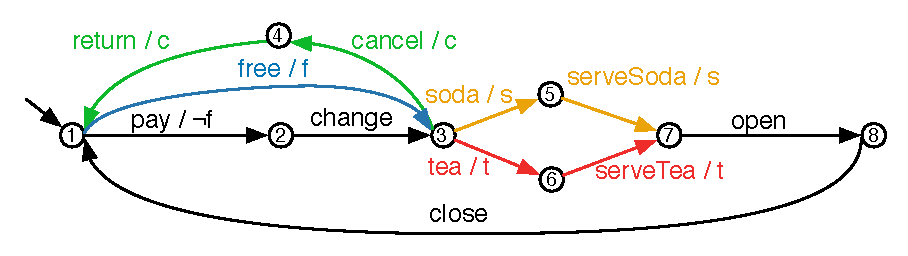
\includegraphics[width = 0.9\linewidth]{figures/fts.pdf}
	\caption{The FTS modeling the vending machine SPL}
	\label{fig:fts-vendingmachine}
\end{figure}

As an illustrative example, Figure~\ref{fig:fts-vendingmachine} depicts an FTS modeling of a product line of vending machines. In addition to an action, a transition in FTS is also labeled with an expression, called \emph{feature expression}, which defines the set of products able to enable this transition. For instance, the transition from state 3 to state 6 is labeled with the feature expression $t$, meaning that it can be executed only by products including the corresponding feature $t$. The transition from state 1 to state 2 is labeled with $\lnot f$, and thus can be executed only by products that do not have the feature $f$. More generally, the expression can be any formula that represents a subset of  products. The transition system representing the behavior  of a particular product is obtained by removing all transitions not available to this product. This operation is named \emph{projection}~\cite{Classen2013}.

Most of FTS-based analyses rely on the annotative model to design efficient CTL and LTL verification algorithms~\cite{Classen2013,Classen2014,Cordy2014}. The result %of these algorithms 
is a feature expression representing all the products that satisfy the property under verification. This feature expression can be represented in different ways. One representation sees a feature expression as two sets of features~\cite{Classen2010}: a set includes the features required to satisfy the property; the other contains the features that must be excluded. Alternatively, feature expressions can be represented as Boolean formulae where included (resp. excluded) features appear as positive (resp. negative) literals~\cite{Classen2013} (as done in Figure~\ref{fig:fts-vendingmachine}). The result of a given verification analysis is another feature expression, produced by computing conjunctions and disjunctions of the individual expressions.

Figure \ref{fig:fts-strategies} illustrates such variability-aware analysis of FTS, where the resulting feature expression is denoted as a Boolean formula.
On the top right corner, an FTS models the behavior of the vending machine product line.
Let us assume that this FTS is checked against the property ``the machine can only \texttt{return} if \texttt{pay} occurred'', which is violated by any product having both free drinks ($f$) and cancel ($c$) features.
Also, we take as example a feature selection for the vending machine selling soda and tea without the free drinks and cancel features.
The family-based analysis step $\hat{\alpha}$ applied to the FTS yields the feature expression $\lnot (c \land f)$. Then, pursuing a family-product-based strategy, one can evaluate this formula under the feature valuation corresponding to the aforementioned product. Doing so would yield $True$, meaning that the product satisfies the property.
Alternatively, one could follow a product-based strategy by projecting the FTS onto the specific product ($\pi$), yielding the transition system shown on the top left corner.
Thus, a classical verification procedure $\alpha$ yields that the product indeed satisfies the property.

\begin{figure}[t]
	\centering
    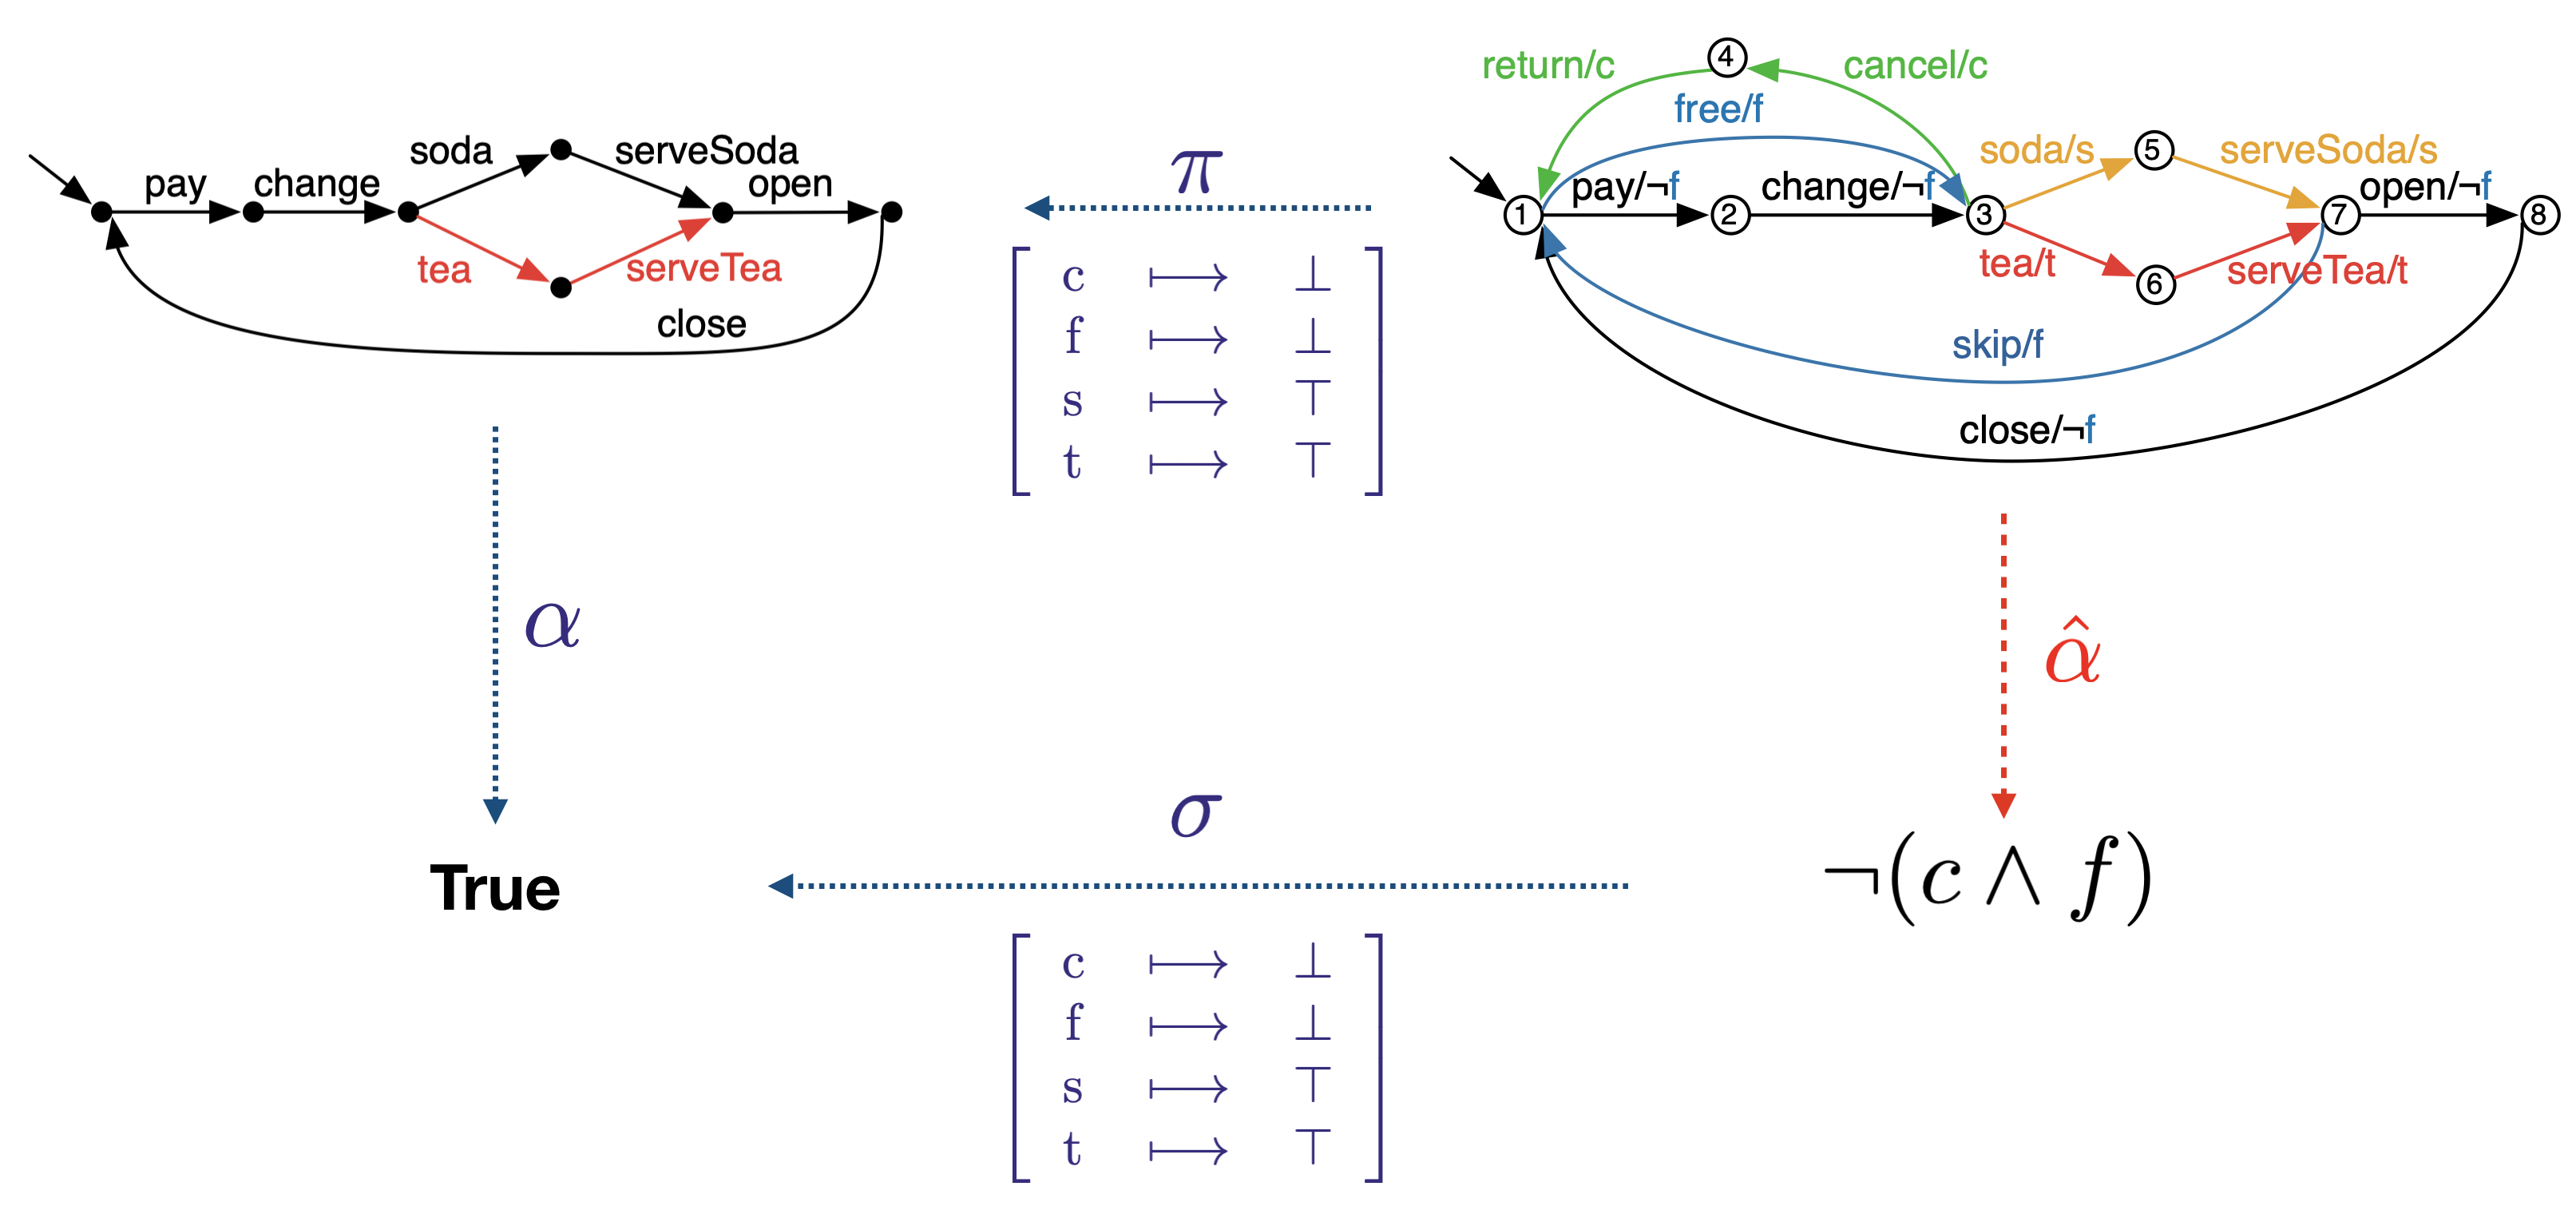
\includegraphics[width = 0.9\linewidth]{figures/fts-strategies.png}
	\caption{Product-based and family-product-based strategies applied to FTS verification}
	\label{fig:fts-strategies}
\end{figure}


Whatever representation one chooses for a feature expression, it can be concisely encoded in a Binary Decision Diagram (BDD)~\cite{Bryant1992,Classen2014}, similar to the ADD encoding of algebraic expressions in \Cref{fig:lifted-expression-example}.
The analysis of \citet{Classen2014} works fully symbolically: both the feature expressions and the state space are encoded as BDDs. The analysis proceeds classically, by induction on the structure of the CTL property, and by computing fixpoints backwards.
Differently, the analysis of \citet{Classen2013} is semi-symbolic: the state space of the model and the automaton of the property are represented explicitly, but the feature expressions are represented as BDDs. Model checking is performed forwards, as in SPIN \cite{Holzmann:2003}, but some states may be re-explored if they are reached with a new combination of features.

%Compositional reasoning on FTS has received less attention. Preliminary work~\cite{Cordy2012,Cordy2012d} studies the particular case where features only add or only remove behavior , and shows what properties are preserved upon the addition of these features. By applying this theory, one can thus infer the impact of each feature successively, and in the end determine which combinations of features lead to violations of the properties. Under the assumption that feature composition is commutative, BDD can again be used as an efficient encoding for these combinations. The general case where features have arbitrary impacts on the FTS remains to be addressed. Several papers deal with the compositional verification of features~\cite{Fisler2005,Liu2011}. Their application to FTS is a future work that is out of scope of this paper.

FTS is a formalism that falls into the category of \emph{annotative} models. Higher-level formalisms are also considered, namely fPromela \cite{Classen2013} (inspired by Promela \cite{Holzmann:2003}). Compositional models also exist. For example, Plath and Ryan~\cite{Plath2001} extended the SMV language to express how a feature modifies an SMV model, called fSMV. 
In fSMV, each feature is modeled in isolation, which paves the way for \emph{compositional} reasoning. \citet{Classen2014} showed that any fSMV model can be transformed into an FTS and vice versa, thereby proving that the compositional model is equivalent to the annotative one. This implies that any verification algorithm designed for one model also works on the other.

\begin{figure}[!htbp]
	\centering
	\begin{tikzpicture}[node distance=80pt and 100pt, align=center, text centered, on grid, scale=0.5]
	\fontsize{10}{12}
	\node (ts) {Transition\\System};
	\node [left= of ts] (fsmv) {SMV + fSMV};
	\node [right= of ts] (fts) {Featured\\Transition\\System};
	
	
	\node [below=of ts] (ctl-ltl) {CTL or LTL \\ (yes / no)};
%	\node [left= of ctl-ltl, below=of fsmv] (compExpr) {$\bot$};
	\node [right= of ctl-ltl, below=of fts] (famExpr) {Feature \\expression};
	
	
	\node [below=of ctl-ltl] (bdd) {BDD};
%	\node [left= of bdd, below=of compExpr] (compLift) {$\bot$};
	\node [right= of bdd, below=of famExpr] (famLift) {Lifted \\feature expression};
	
	\draw[product] (featModel) -- node [midway, above] {$\pi'$} (ts);
	\draw[product] (fts) -- node [midway, above] {$\pi$} (ts);
	\draw[family, <->] (featModel) to [bend left=25] node [midway, above] {$\gamma$} (famModel);
	
%	\draw[feature] (featModel) -- node [midway, left] {$\bot$} (featExpr);
	\draw[family] (fts) -- node [midway, right] {$\hat{\alpha}$} (famExpr);
	\draw[product] (ts) to node [midway, left] {$\alpha$} (ctl-ltl);
	
%	\draw[product] (featExpr) -- node [midway, above] {$\bot$} (reliability);
	\draw[product] (famExpr) -- node [midway, above] {$\sigma$} (ctl-ltl);
	%\draw[family] (featExpr) to [bend left=25] node [near end, above] {\hyperref[def:variability-encoding-function-expressions]{$\gamma$}} (famExpr);
	
%	\draw[family] (featExpr) -- node [midway, left] {$\bot$} (featLift);
	\draw[family] (famExpr) -- node [midway, right] {$\mathit{lift}$} (famLift);
	\draw[product] (bdd) to node [near start, left] {$\llbracket \_ \rrbracket_c$} (ctl-ltl);
	
%	\draw[family] (featLift) -- node [midway, above] {$\bot$} (bdd);
	\draw[family] (famLift) -- node [midway, above] {$\hat{\sigma}$} (bdd);
	
	\node [below= 25pt of bdd] (anchor) {};
	\node [left= 62pt of anchor.north, anchor=north west, draw=black, rounded corners=2pt, font=\scriptsize] (legend) {
		\settowidth{\columnLength}{FTS model checking checking}
		\begin{tabular}{ll|ll}
		$\pi$                    & projection \cite{Classen2013}  & $\pi'$ & feature composition~\cite{Plath2001} \\
		$\sigma$                     & product evaluation      & $\hat{\sigma}$  & BDD evaluation \\
		$\alpha$                     & model checking  & $\hat{\alpha}$  & FTS model checking~\cite{Classen2013,Classen2014} \\
		$\llbracket \_ \rrbracket_c$ & BDD application & $\gamma$ & lifted composition~\cite{Classen2014}\\
		$\mathit{lift}$ & maps expression into BDD semantics & \\ %$\bot$ & unexplored
		% & & $\delta$ & compositional reasoning
		\end{tabular}};
	\node [left= 10pt of legend.north west, anchor=north east, draw=black, rounded corners=2pt, font=\footnotesize] (legendStrat) {
		\begin{tabular}{ll}
		\raisebox{2pt}{\tikz{\draw[feature](0,0) -- (5mm,0);}} & feature-based\\
		\raisebox{2pt}{\tikz{\draw[family](0,0) -- (5mm,0);}} & family-based\\
		\raisebox{2pt}{\tikz{\draw[product](0,0) -- (5mm,0);}} & product-based
		\end{tabular}};
	\end{tikzpicture}
	\caption{Commutative diagram of product-line behavioral properties  verification strategies}
	\label{fig:diagram-FTS}
\end{figure}

\paragraph{Summary}
The above review of the state of the art of FTS verification suggests partial reuse of the structure of the commutative diagram in Figure~\ref{fig:strategies-overview}, resulting in Figure~\ref{fig:diagram-FTS}. From an FTS (see top right of Figure~\ref{fig:diagram-FTS}), one can pursue a product-based strategy by computing the projection ($\pi$) of each product and applying a standard model checking algorithm ($\alpha$). In contrast, family-based strategies start with the application of dedicated algorithms to FTS ($\hat{\alpha}$) to obtain the set of products satisfying the property. This set can either be enumerated ($\sigma$), giving rise to a family-product-based strategy, or lifted into a feature expression encoded in BDD semantics and then being evaluated without enumeration into a BDD ($\hat{\sigma}$).

On the other side, one finds the aforementioned fSMV model of Plath and Ryan~\cite{Plath2001}. The transition system of a particular product can be obtained by composing the base model with the model of each of its features ($\pi')$. A family-based approach can be followed to produce directly an FTS from the \emph{lifted composition}~\cite{Classen2014} of the base model and all the features ($\gamma$). Feature-based strategies have been proposed under specific assumptions (e.g., that features only add behavior) \cite{Cordy2012}, but do not apply outside such restricted scope. 
The soundness of the analyses is proved by the commutativity of the upper-right quadrant of Figure~\ref{fig:diagram-FTS} and by the equivalence result by~\citet{Classen2014}, similarly to Figure~\ref{fig:family-product-example}.

%\begin{figure}[!htbp]
%\centering
%\begin{tikzpicture}[node distance=80pt and 100pt, align=center, text centered, on grid, scale=0.5]
%    \fontsize{10}{12}
%    \node (dtmc) {DTMC};
%    \node [left= of dtmc, text width=70pt] (featModel) {\hyperref[def:feature-based-probabilistic-model]{Compositional model}};
%    \node [right= of dtmc, text width=70pt] (famModel) {\hyperref[def:150fdtmc]{Annotative model}};
%
%%    \node [below right=30pt and 50pt of featModel, text=gray] (featProdSound) {\footnotesize\Cref{theorem:feature-product-soundness}};
%%    \node [below left=30pt and 50pt of famModel, text=gray] (famProdSound) {\footnotesize\Cref{theorem:family-product-soundness}};
%%    \node [above=20pt of dtmc, text=gray] (varEnc) {\footnotesize\Cref{theorem:variability-encoding-soundness}};
%
%    \node [below=of dtmc] (reliability) {Reliability};
%    \node [left= of reliability, below=of featModel] (featExpr) {Compositional\\expressions};
%    \node [right= of reliability, below=of famModel] (famExpr) {Annotative\\expression};
%%    \node [above=20pt of reliability, text=gray] (varEncExpr) {\footnotesize\Cref{theorem:variability-encoding-expressions-soundness}};
%%
%%    \node [below right=40pt and 50pt of featExpr, text=gray] (featFamSound) {\footnotesize\Cref{theorem:feature-family-soundness}};
%%    \node [below left=40pt and 50pt of famExpr, text=gray] (famSound) {\footnotesize\Cref{theorem:family-soundness}};
%
%    \node [below=of reliability] (reliabilityADD) {Reliability\\ADD};
%    \node [left= of reliabilityADD, below=of featExpr] (featLift) {Compositional\\lifted expressions};
%    \node [right= of reliabilityADD, below=of famExpr] (famLift) {Annotative\\lifted expression};
%
%    \draw[product] (featModel) -- node [midway, above] {\hyperref[def:derivation-by-composition]{$\lambda'$}} (dtmc);
%    %\draw[product] (featModel) to [bend right=10] node [midway, below] {\hyperref[def:fdtmc-derivation]{$\lambda$}} (dtmc);
%    \draw[product] (famModel) -- node [midway, above] {\hyperref[def:fdtmc-derivation]{$\lambda$}} (dtmc);
%    \draw[family] (featModel) to [bend left=25] node [midway, above] {\hyperref[def:variability-encoding-function]{$\lambda_v$}} (famModel);
%
%    \draw[feature] (featModel) -- node [midway, left] {\hyperref[def:alpha_v]{$\alpha_v$}} (featExpr);
%    \draw[family] (famModel) -- node [midway, right] {\hyperref[def:alpha_v]{$\alpha_v$}} (famExpr);
%    \draw[product] (dtmc) to node [midway, left] {\hyperref[def:alpha]{$\alpha$}} (reliability);
%
%    \draw[product] (featExpr) -- node [midway, above] {\hyperref[def:sigma]{$\sigma$}} (reliability);
%    \draw[product] (famExpr) -- node [midway, above] {\hyperref[def:sigma]{$\sigma$}} (reliability);
%    \draw[family] (featExpr) to [bend left=25] node [near end, above] {\hyperref[def:variability-encoding-function-expressions]{$\lambda_v$}} (famExpr);
%
%    \draw[family] (featExpr) -- node [midway, left] {\hyperref[def:lift]{$\mathit{lift}$}} (featLift);
%    \draw[family] (famExpr) -- node [midway, right] {\hyperref[def:lift]{$\mathit{lift}$}} (famLift);
%    \draw[product] (reliabilityADD) to node [near start, left] {$\llbracket \_ \rrbracket_c$} (reliability);
%
%    \draw[family] (featLift) -- node [midway, above] {\hyperref[def:sigma_v]{$\sigma_v$}} (reliabilityADD);
%    \draw[family] (famLift) -- node [midway, above] {\hyperref[def:sigma_v]{$\sigma_v$}} (reliabilityADD);
%
%    \node [below= 25pt of reliabilityADD] (anchor) {};
%    \node [left= 62pt of anchor.north east, anchor=north west, draw=black, rounded corners=2pt, font=\scriptsize] (legend) {
%        \newlength{\columnLength}
%        \settowidth{\columnLength}{evaluation with ADDs}
%        \begin{tabular}{ll|ll}
%            $\lambda$                    & derivation      & $\lambda_v$ & variability encoding \\
%            $\sigma$                     & evaluation      & $\sigma_v$  & evaluation with ADDs \\
%            $\alpha$                     & model checking  & $\alpha_v$  & \multirow{2}{\columnLength}{parametric model checking} \\
%            $\llbracket \_ \rrbracket_c$ & ADD application &             &
%        \end{tabular}};
%    \node [left= 10pt of legend.north west, anchor=north east, draw=black, rounded corners=2pt, font=\footnotesize] (legendStrat) {
%        \begin{tabular}{ll}
%            \raisebox{2pt}{\tikz{\draw[feature](0,0) -- (5mm,0);}} & feature-based\\
%            \raisebox{2pt}{\tikz{\draw[family](0,0) -- (5mm,0);}} & family-based\\
%            \raisebox{2pt}{\tikz{\draw[product](0,0) -- (5mm,0);}} & product-based
%        \end{tabular}};
%\end{tikzpicture}
%\caption{Commutative diagram of product-line reliability analysis strategies}
%\label{fig:strategies-overview}
%\end{figure}

%In the remaining sections, we detail each of these strategies and analysis steps with the goal of making statements about their commuting relations.
%\Cref{sec:product} presents product-based analysis strategies for both annotative and compositional models, with the goal of establishing a baseline
%for the remaining soundness proofs.
%\Cref{sec:family-star} discusses family-product-based and family-based analyses of annotative models.
%Feature-product-based and feature-family-based analysis strategies are the subject of \Cref{sec:feature-star}, which focuses on compositional models.
%Finally, \Cref{sec:variability-encoding} bridges the gap between analyses of annotative and compositional models (function $\lambda_v$ in
%\Cref{fig:strategies-overview}), establishing their commutativity.
%
%
%\subsection{Product-based Strategies}
%\label{sec:product}
%
%Product-based analysis strategies are based on the analysis of generated products or models thereof~\cite{Thum2014}.
%In \Cref{sec:model-representations}, we have discussed how to represent probabilistic behavioral models of product lines as PMCs,
%using both annotative and compositional approaches.
%There, we also described how to derive models of individual products, both for the annotative and the compositional approaches.
%The generated models are plain DTMCs, that is, their variability has been resolved at derivation time.
%Thus, to analyze the generated models, one only needs to model-check the non-parametric probabilistic reachability for every such model.
%We hereafter denote this non-parametric model checking analysis step by the following function $\alpha$.
%
%\begin{definition}[Non-parametric model checking]
%\label{def:alpha}
%    The non-para\-met\-ric mod\-el checking step $\alpha: DTMC \to [0,1]$ consists of applying the algorithm by \citet{HahnHZ10}.
%    For a DTMC $\mathcal{D} =$ \dtmc{},
%    $$\alpha(\mathcal{D}) = Pr^{\mathcal{D}}(s_0, T)$$
%    Since a DTMC has no parameters, $\alpha$ yields constant functions, which we interpret as plain Real numbers.
%\end{definition}
%
%Although there are more efficient algorithms for reliability model checking of regular (non-parametric) DTMCs,
%we use the algorithm by \citet{HahnHZ10} in the above definition for uniformity, which eases understanding.
%Since this algorithm is sound (\Cref{lemma:pmc-soundness}), a working implementation of the presented theory is free
%to exploit another sound probabilistic reachability algorithm for performance reasons.
%
%Now we are able to define product-based analysis for annotative and compositional models.
%\begin{definition}[Product-based analysis of annotative models]
%\label{def:product-annotative}
%%References: def:150fdtmc, def:fdtmc-derivation, def:alpha
%    Given an annotative model \annotativeModel{}, a product-based analysis yields, for all $c \in \llbracket \mathit{FM} \rrbracket$,
%    $$\alpha(\lambda(\mathcal{P}, w, c))$$
%    or, alternatively,
%    $$\alpha(\llbracket \mathcal{P} \rrbracket^w_c)$$
%\end{definition}
%\begin{definition}[Product-based analysis of compositional models]
%\label{def:product-compositional}
%    Given a compositional model \compositionalModel{}, a product-based analysis yields, for all $c \in \llbracket \mathit{FM} \rrbracket$,
%    $$\alpha(\lambda'(\mathcal{P_\top}, w', c))$$
%    where $\mathcal{P_\top}$ is the maximal PMC in $\mathscr{P}$ under $\prec$.
%\end{definition}
%
%So, a product-based analysis results in a mapping from configurations to respective reliability values, such as
%$\{c \mapsto \alpha(\lambda(\mathcal{P}, w, c)) \;|\; c \in \llbracket \mathit{FM} \rrbracket\}$ for annotative models, for instance.
%%Nonetheless, we focus on the results for individual configurations both for simplicity and because it is sufficient to
%%make statements about commutativity with other strategies.
%
%\begin{framed}
%    Both analysis strategies presented in this \namecref{sec:product} derive models for individual products of a given
%    product line and then apply a single-product analysis technique as is.
%    Since single-product analyses represent the base case upon which product-line analyses are built, the product-based
%    strategies establish a baseline for proving the soundness of other strategies.
%\end{framed}
%
%
%\subsection{Family-based Strategies}
%\label{sec:family-star}
%
%According to \citet{Thum2014}, a family-based analysis strategy is one that (a) operates only on domain artifacts and
%that (b) incorporates the knowledge about valid feature combinations.
%In this \namecref{sec:family-star}, we explore this kind of strategy in the context of annotative probabilistic models,
%because they encode the behavior of all products of a product line in a single PMC.
%It is also possible to perform family-based analyses on a compositional model by first transforming it into an annotative
%one, but this is discussed later in \Cref{sec:variability-encoding}.
%
%First, we show how to perform an analysis that yields a reliability expression, which can in turn be evaluated
%for each valid configuration of the product line.
%This characterizes a family-product-based strategy (\Cref{sec:family-product}).
%Then, the aforementioned analysis is leveraged to build a pure family-based (i.e., non-enumerative) strategy (\Cref{sec:family}).
%At first, it may seem counterintuitive to present the family-product-based approach before the family-based one.
%However, we shall see that our pure family-based approach builds upon concepts of the hybrid family-product-based approach, and that
%performing one or the other is a matter of choosing product-based or family-based analysis steps after a preliminary family-based step.
%
%\subsubsection{Family-product-based Strategy}
%\label{sec:family-product}
%
%A family-product-based strategy is a family-based strategy followed by a prod\-uct-based strategy over intermediate results~\cite{Thum2014}.
%%After defining the mechanics of the specific family-product-based strategy described in this section, we prove its correctness by comparing it
%%to perfoming a naïve product-based strategy (i.e., generate every product and analyze each of them separately).
%The preliminary family-based step of our family-product-based analysis consists of applying parametric model checking of probabilistic
%reachability (\Cref{sec:probabilistic-reachability}) of the underlying PMC of the annotative model.
%This step is abstracted as a function $\alpha_v$, where the subscript $v$ denotes that it is a variability-aware version of the non-parametric
%model checking function $\alpha$ (\Cref{def:alpha}).
%\begin{definition}[Parametric model checking]
%\label{def:alpha_v}
%    The parametric model checking analysis step $\alpha_v: PMC_X \to \mathcal{F}_X$ consists of applying the algorithm by
%    \citet{HahnHZ10} for probabilistic reachability, which yields a rational expression $\varepsilon \in \mathcal{F}_X$ for a PMC
%    with variables set $X$.
%    For a PMC $\mathcal{P} =$ \pmc{}, the input target states of the algorithm are the ones in $T$.
%\end{definition}
%
%After performing parametric model checking, the result of reachability analysis is an expression over the same variables as the
%annotative input PMC, denoting the PMC's reliability as a function of these variables.
%Hence, we expect this annotative reliability expression to be evaluated using the same evaluation functions that restricted the possible behaviors
%in the original model.
%This \emph{expression evaluation}, which can be seen as model derivation applied to expressions, is captured in function $\sigma$.
%\begin{definition}[Expression evaluation]
%\label{def:sigma}
%    Given an expression $\varepsilon$ over a set $X$ of variables, an evaluation factory $w$,
%    and a configuration $c \in \llbracket \mathit{FM} \rrbracket$,
%    we define the expression evaluation function in a similar fashion as DTMC derivation:
%    $$\sigma(\varepsilon, w, c) = \varepsilon[X/w(c)]$$
%    Likewise, we can use $\llbracket \varepsilon \rrbracket^w_c$ to denote $\sigma(\varepsilon, w, c)$.
%\end{definition}
%
%The function $\sigma$ is applied to the reliability expression for all valid configurations of the product line,
%yielding the final product-based step.
%The resulting family-product-based approach for the analysis of annotative models is then defined as follows.
%\begin{definition}[Family-product-based analysis]
%\label{def:family-product}
%%References: def:alpha_v, def:sigma, def:150fdtmc
%    Given an annotative model \annotativeModel{}, the family-product-based analysis yields, for all $c \in \llbracket \mathit{FM} \rrbracket$,
%    $$\sigma(\alpha_v(\mathcal{P}), w, c)$$
%    or, alternatively,
%    $$\llbracket \alpha_v(\mathcal{P}) \rrbracket^w_c$$
%\end{definition}
%
%\Cref{fig:family-product-example} illustrates the family-product-based strategy in contrast with the product-based one
%(\Cref{sec:product}), providing an intuition for why they commute.
%DTMC derivation $\lambda$ and expression evaluation $\sigma$ are both performed for a configuration $c$ such that $c \models p_x$.
%This way, $w(c)(x) = 1$ and the reliability is $0.9801$.
%If $c$ were such that $x$ was absent (i.e., $c \not \models p_x$), then the reliability would be $0.99$.
%
%\begin{figure}[!htbp]
%    \centering
%    \begin{tikzpicture}[node distance=20pt and 20pt,
%                        align=center,
%                        text centered]%, on grid]
%        \scriptsize
%        \node [draw, circle] (s0) {$s_0$};
%        \node [draw, circle, right= of s0] (s1) {$s_1$};
%        \node [draw, circle, right= of s1] (s2) {$s_2$};
%        \node [draw, circle, right= of s2] (ssuc) {$s_{\mathit{suc}}$};
%        \node [draw, circle, below= of ssuc] (serr) {$s_{\mathit{err}}$};
%
%        \draw[->] (s0) to node [midway, above] {$0.99$} (s1);
%        \draw[->] (s0) to [bend right=25] node [near start, right] {$0.01$} (serr);
%        \draw[->] (s1) to node [midway, above] {$\mathbf{x}$} (s2);
%        \draw[->] (s1) to [bend left=35] node [midway, above] {$\mathbf{1-x}$} (ssuc);
%        \draw[->] (s2) to node [midway, above] {$0.99$} (ssuc);
%        \draw[->] (s2) to [bend right=25] node [near start, right] (shortlab) {$0.01$} (serr);
%        \draw[->] (ssuc) to [loop right, in=30, out=330, looseness=4] node [midway, right] (ssuclab) {$1$} (ssuc);
%        \draw[->] (serr) to [loop right, in=30, out=330, looseness=4] node [midway, right] (serrlab) {$1$} (serr);
%
%        \node [draw=none, rectangle, fit=(s0) (ssuc) (serrlab) (serr) (shortlab)] (fdtmc) {};
%
%        \node [draw, circle, below= 80pt of s0] (ss0) {$s_0$};
%        \node [draw, circle, right= of ss0] (ss1) {$s_1$};
%        \node [draw, circle, right= of ss1] (ss2) {$s_2$};
%        \node [draw, circle, right= of ss2] (sssuc) {$s_{\mathit{suc}}$};
%        \node [draw, circle, below= of sssuc] (sserr) {$s_{\mathit{err}}$};
%
%        \draw[->] (ss0) to node [midway, above] {$0.99$} (ss1);
%        \draw[->] (ss0) to [bend right=25] node [near start, right] {$0.01$} (sserr);
%        \draw[NewEdge] (ss1) to node [midway, above] {$1$} (ss2);
%        \draw[RemovedEdge] (ss1) to [bend left=35] node [midway, above] (sshortlab) {$0$} (sssuc);
%        \draw[->] (ss2) to node [midway, above] {$0.99$} (sssuc);
%        \draw[->] (ss2) to [bend right=25] node [near start, right] {$0.01$} (sserr);
%        \draw[->] (sssuc) to [loop right, in=30, out=330, looseness=4] node [midway, right] (sssuclab) {$1$} (sssuc);
%        \draw[->] (sserr) to [loop right, in=30, out=330, looseness=4] node [midway, right] (sserrlab) {$1$} (sserr);
%
%        \node [draw=none, rectangle, fit=(ss0) (sssuc) (sserrlab) (sserr) (sshortlab)] (dtmc) {};
%
%        \normalsize
%        \node [right= 50pt of fdtmc] (expr) {$0.9801\cdot x + 0.99\cdot(1-x)$};
%        \node at (expr|-dtmc) (reliability) {$0.9801$};
%
%        \draw[product] (fdtmc) to node [midway, left] {\hyperref[def:fdtmc-derivation]{$\lambda$}} (dtmc);
%        \draw[family] (fdtmc) to node [midway, above] {\hyperref[def:alpha_v]{$\alpha_v$}} (expr);
%        \draw[product] (dtmc) to node [midway, below] {\hyperref[def:alpha]{$\alpha$}} (reliability);
%        \draw[product] (expr) to node [midway, right] {\hyperref[def:sigma]{$\sigma$}} (reliability);
%    \end{tikzpicture}
%    \caption{
%        Example of family-product-based analysis ($\alpha_v$ followed by $\sigma$) in contrast to a
%        product-based analysis ($\lambda$ followed by $\alpha$) of an annotative PMC
%    }
%    \label{fig:family-product-example}
%\end{figure}
%
%To be considered sound, a family-product-based analysis must be equivalent to performing a product-based analysis of all products.
%This means that performing a parametric model checking step and then evaluating the resulting expression for each valid product
%must yield the same result as first deriving the original annotative model for each product and then performing non-parametric
%model checking on each resulting DTMC.
%To prove that this equivalence holds, we can leverage a more general result about PMCs and well-defined evaluations.
%
%\begin{lemma}[Commutativity of PMC and expression evaluations]
%\label{lemma:evaluations-commute}
%    Given any PMC $\mathcal{P} =$ \pmc{} and a well-defined evaluation $u$, it holds that
%    $$\alpha(\mathcal{P}[X/u]) = \alpha_v(\mathcal{P})[X/u]$$
%\end{lemma}
%\begin{proof}
%    \begin{align*}
%        \alpha(\mathcal{P}[X/u]) &= \alpha(\mathcal{P}_{u}) &\text{(syntax change)} \\
%                                 &= Pr^{\mathcal{P}_{u}}(s_0, T) &\text{(\Cref{def:alpha})} \\
%                                 \shortintertext{and, since $u$ is well-defined,}
%                                 &= \alpha_v(\mathcal{P})[X/u] &\text{(\Cref{lemma:pmc-soundness} and \Cref{def:alpha_v})}
%    \end{align*}
%\end{proof}
%
%Using this result, we are able to express the soundness of the family-product-based approach
%in the following \namecref{theorem:family-product-soundness}.
%
%\begin{theorem}[Soundness of family-product-based analysis]
%\label{theorem:family-product-soundness}
%%References: def:150fdtmc, def:family-product, def:alpha, def:sigma, def:alpha_v, def:product-annotative
%    Given an annotative model \annotativeModel{}, for all $c \in \llbracket \mathit{FM} \rrbracket$
%    $$\alpha(\llbracket \mathcal{P} \rrbracket^w_c) = \llbracket \alpha_v(\mathcal{P}) \rrbracket^w_c$$
%    Alternatively, $ \alpha(\lambda(\mathcal{P}, w, c)) = \sigma(\alpha_v(\mathcal{P}), w, c) $.
%\end{theorem}
%\begin{proof}
%    Since $w(c)$ is a well-defined evaluation (\Cref{lemma:150fdtmc-w-well-defined}), we can use it to instantiate
%    $u$ in \Cref{lemma:evaluations-commute}.
%    Thus, let $\mathcal{P} =$ \pmc{}.
%    \begin{align*}
%        \alpha(\llbracket \mathcal{P} \rrbracket^w_c) &= \alpha(\mathcal{P}[X/w(c)]) &\text{(\Cref{def:fdtmc-derivation})} \\
%                                                      &= \alpha_v(\mathcal{P})[X/w(c)] &\text{(\Cref{lemma:evaluations-commute,lemma:150fdtmc-w-well-defined})} \\
%                                                      &= \llbracket \alpha_v(\mathcal{P}) \rrbracket^w_c &\text{(\Cref{def:sigma})}
%    \end{align*}
%\end{proof}
%
%\begin{framed}
%    As a major result, \Cref{theorem:family-product-soundness} states that the diagram in \Cref{fig:family-product-soundness} commutes.
%    This diagram corresponds to the upper right quadrant in \Cref{fig:strategies-overview}.
%\end{framed}
%
%\begin{figure}[!htbp]
%    \centering
%    \begin{tikzpicture}[node distance=80pt and 100pt, align=center, text centered, on grid]
%        \fontsize{10}{12}
%        \node (dtmc) {DTMC};
%        \node [above=50pt of dtmc, text width=50pt] (famModel) {\hyperref[def:150fdtmc]{Annotative model}};
%
%        \node [right=of dtmc] (reliability) {Reliability};
%        \node [above=50pt of reliability, right=of famModel] (famExpr) {Annotative\\expression};
%
%        \draw[product] (famModel) -- node [midway, left] {\hyperref[def:fdtmc-derivation]{$\lambda$}} (dtmc);
%        \draw[family] (famModel) -- node [midway, above] {\hyperref[def:alpha_v]{$\alpha_v$}} (famExpr);
%        \draw[product] (dtmc) to node [midway, below] {\hyperref[def:alpha]{$\alpha$}} (reliability);
%        \draw[product] (famExpr) -- node [midway, right] {\hyperref[def:sigma]{$\sigma$}} (reliability);
%    \end{tikzpicture}
%    \caption{Statement of \Cref{theorem:family-product-soundness}}
%    \label{fig:family-product-soundness}
%\end{figure}
%
%\subsubsection{Family-based Strategy}
%\label{sec:family}
%
%The pure family-based strategy starts by applying parametric model checking to the given annotative model, as in the family-based step
%of the family-product-based strategy.
%However, instead of evaluating the resulting expression for each variant, we \emph{lift} it to an ADD-based reliability expression,
%which can be evaluated for all variants at once.
%While an expression is evaluated with real values, a lifted expression is evaluated using ADDs, which represent
%Boolean functions from features to real values.
%Each of these ADDs encode the values that a variable can assume according to each possible configuration, also known as
%\emph{variational data}~\cite{VariationalDataStructures}.
%Since this approach incorporates the knowledge of valid feature combinations, it is a family-based strategy.
%
%Let us take the vending machine product line (\Cref{fig:complete-annotative-vending-machine}) as an example.
%Its reliability expression after parametric model checking has 8 terms, one of which is $0.124659 \cdot t \cdot t_\mathit{taste}$.
%Starting from the evaluation factory $w$, we can derive functions $\psi_x$ that, for each variable $x$, take a configuration
%$c \in \llbracket \mathit{FM} \rrbracket$ as input and output the corresponding value $w(c)(x)$.
%For $t$ and $t_\mathit{taste}$, for instance, these functions would be as follows:
%\begin{align*}
%    \psi_t(      \mathtt{Tea}, \lnot \mathtt{Soda}, \lnot \mathtt{Taste}) &= 1   &\psi_{t_\mathit{taste}}(      \mathtt{Tea}, \lnot \mathtt{Soda}, \lnot \mathtt{Taste})  &= 0 \\
%    \psi_t(      \mathtt{Tea}, \lnot \mathtt{Soda},       \mathtt{Taste}) &= 1   &\psi_{t_\mathit{taste}}(      \mathtt{Tea}, \lnot \mathtt{Soda},       \mathtt{Taste})        &= 1 \\
%    \psi_t(\lnot \mathtt{Tea},       \mathtt{Soda}, \lnot \mathtt{Taste}) &= 0   &\psi_{t_\mathit{taste}}(\lnot \mathtt{Tea},       \mathtt{Soda}, \lnot \mathtt{Taste})  &= 0 \\
%    \psi_t(\lnot \mathtt{Tea},       \mathtt{Soda},       \mathtt{Taste}) &= 0   &\psi_{t_\mathit{taste}}(\lnot \mathtt{Tea},       \mathtt{Soda},       \mathtt{Taste})        &= 0
%\end{align*}
%Having each of these functions represented by an ADD enables the efficient computation of the reliability expression as another ADD $\hat{r}$,
%representing a Boolean function that could be defined pointwise as
%$\hat{r}(c) = 0.124659 \cdot \psi_t(c) \cdot \psi_{t_\mathit{taste}}(c)$
%(we omit the remaining terms for simplicity).
%
%We now formally define expression lifting, as well as the mechanics of generating ADD-based evaluations and evaluating lifted expressions.
%
%\begin{definition}[Expression lifting]
%\label{def:lift}
%    For a given rational expression $\varepsilon \in \mathcal{F}_X$, whose semantics is a rational function $\mathbb{R}^{|X|} \to \mathbb{R}$,
%    and a product line with $k$ features,
%    we define the lifted expression $\mathit{lift}(\varepsilon) = \hat{\varepsilon}$ as an expression which is syntactically equal
%    to $\varepsilon$, but whose semantics
%    is lifted to a rational function $(\mathbb{B}^k \to \mathbb{R})^{|X|} \to (\mathbb{B}^k \to \mathbb{R})$, such that:
%
%    \begin{itemize}
%        \item
%            The function's inputs are $k$-ary ADDs.
%        \item
%            Polynomial coefficients are interpreted as constant ADDs (e.g., the number $5$ becomes $c \in \mathbb{B}^k \mapsto 5$).
%            We denote a constant $a$ lifted to a constant ADD as $\hat{a}$, so that $\hat{a}(\bar{b}) = a$ (where $\bar{b}$ is a Boolean tuple).
%        \item
%            Arithmetic operators are lifted to their ADD-based counterparts.
%    \end{itemize}
%    Hence, the admitted evaluations for $\hat{\varepsilon}$ are of type $u: X \to (\mathbb{B}^k \to \mathbb{R})$,
%    so that variables are properly replaced by $k$-ary ADDs.
%\end{definition}
%
%By the above definition, lifted expressions are syntactically equal to their original (non-lifted) counterparts.
%However, instead of using Real arithmetics, we interpret operators, constants, and variables using ADDs and ADD arithmetics (\Cref{sec:ADD}).
%These semantically lifted expressions are sound in the sense that they denote functions that, when evaluated with a given configuration,
%yield the same results as if the variables of the original expressions would have been individually evaluated for the same configuration.
%
%\begin{lemma}[Soundness of expression lifting]
%\label{lemma:lifting-soundness}
%    If $\varepsilon$ is a rational expression over Real constants and variables $x_i \in X$,
%    $|X| = n$, $A_1,\dotsc,A_n$ are ADDs,
%    and $\hat{\varepsilon} = \mathit{lift}(\varepsilon)$, then
%    $$ \hat{\varepsilon}[x_1/A_1,\dotsc,x_n/A_n](\bar{b}) = \varepsilon[x_1/A_1(\bar{b}), \dotsc, x_n/A_n(\bar{b})] $$
%    where $\bar{b}$ is a vector of $k$ Booleans, corresponding to a selection of the $k$ features in a given product line.
%\end{lemma}
%\begin{proof}
%
%    The proof is by structural induction on expression $\varepsilon$.
%    The base cases are constant expressions and single variables:
%    \begin{itemize}
%        \item
%            $\varepsilon = c$, where $c \in \mathbb{R}$:
%
%            In this case, $\hat{\varepsilon} = \hat{c}$.
%            Since $\varepsilon$ has no variables (and neither has $\hat{\varepsilon}$), we apply the empty evaluation $[\;]$.
%            Thus, $\hat{\varepsilon}[\;](\bar{b}) = \hat{c}(\bar{b}) = c = \varepsilon = \varepsilon[\;]$.
%
%        \item
%            $\varepsilon = x$:
%
%            In this case, $\hat{\varepsilon} = x$.
%            If $A$ is an arbitrary ADD, then:
%            $\hat{\varepsilon}[x/A](\bar{b}) = A(\bar{b}) = \varepsilon[x/A(\bar{b})]$.
%    \end{itemize}
%
%    As induction hypothesis, for the expressions $\varepsilon = \varepsilon_1$ and $\varepsilon = \varepsilon_2$,
%    assume that the following holds:
%    \begin{equation*}
%        \tag{I.H.}
%        \hat{\varepsilon}[x_1/A_1,\dotsc,x_n/A_n](\bar{b}) = \varepsilon[x_1/A_1(\bar{b}), \dotsc, x_n/A_n(\bar{b})]
%    \end{equation*}
%    Let $u: X \to (\mathbb{B}^k \to \mathbb{R})$ be a lifted evaluation such that $u(x_i) = A_i$ is an ADD.
%    Since $\varepsilon$ is a rational expression (i.e., a quotient of polynomials, as yielded by a parametric model checking algorithm---see
%    \Cref{sec:pmc,sec:probabilistic-reachability}),
%    it involves only the four basic arithmetic operators and exponentiation to Natural powers.
%    Thus, we examine the cases where we perform ADD arithmetics (\Cref{sec:ADD}), corresponding to the allowed operations in $\varepsilon$:
%    \begin{itemize}
%        \item
%            $\varepsilon = \varepsilon_1 \odot \varepsilon_2$, where $\odot \in \{+, -, \times, \div\}$:
%
%            In this case, $\hat{\varepsilon} = \hat{\varepsilon_1} \odot \hat{\varepsilon_2}$.
%            Hence,
%            \begin{align*}
%                \hat{\varepsilon}[X/u](\bar{b}) &= \big( \hat{\varepsilon_1} \odot \hat{\varepsilon_2} \big)[X/u](\bar{b})      & \\
%                                                &= \big( \hat{\varepsilon_1}[X/u] \odot \hat{\varepsilon_2}[X/u] \big)(\bar{b}) & \text{(evaluation)} \\
%                                                &= \hat{\varepsilon_1}[X/u](\bar{b}) \odot \hat{\varepsilon_2}[X/u](\bar{b})    & \text{(ADD arithmetics)} \\
%                                                &= \hat{\varepsilon_1}[x_1/A_1,\dotsc,x_n/A_n](\bar{b}) & \\
%                                                & \qquad \odot \hat{\varepsilon_2}[x_1/A_1,\dotsc,x_n/A_n](\bar{b})    & \text{(expanding $u$)} \\
%                                                &= \varepsilon_1[x_1/A_1(\bar{b}),\dotsc,x_n/A_n(\bar{b})] & \\
%                                                & \qquad \odot \varepsilon_2[x_1/A_1(\bar{b}),\dotsc,x_n/A_n(\bar{b})]    & \text{(induction hypothesis)} \\
%                                                &= \big( \varepsilon_1 \odot \varepsilon_2 \big)[x_1/A_1(\bar{b}),\dotsc,x_n/A_n(\bar{b})]    & \text{(evaluation)} \\
%                                                &= \varepsilon[x_1/A_1(\bar{b}),\dotsc,x_n/A_n(\bar{b})]    &
%            \end{align*}
%
%        \item
%            $\varepsilon = \varepsilon_1^i$, where $i \in \mathbb{N}$:
%
%            In this case, $\hat{\varepsilon} = \hat{\varepsilon_1}^i$.
%            Hence,
%            \begin{align*}
%                \hat{\varepsilon}[X/u](\bar{b}) &= \hat{\varepsilon_1}^i[X/u](\bar{b})                          & \\
%                                                &= \hat{\varepsilon_1}[X/u]^i(\bar{b})                          & \text{(evaluation)} \\
%                                                &= \hat{\varepsilon_1}[X/u](\bar{b})^i                          & \text{(ADD arithmetics)} \\
%                                                &= \hat{\varepsilon_1}[x_1/A_1,\dotsc,x_n/A_n](\bar{b})^i       & \text{(expanding $u$)} \\
%                                                &= \varepsilon_1[x_1/A_1(\bar{b}),\dotsc,x_n/A_n(\bar{b})]^i    & \text{(induction hypothesis)} \\
%                                                &= \varepsilon_1^i[x_1/A_1(\bar{b}),\dotsc,x_n/A_n(\bar{b})]    & \text{(evaluation)} \\
%                                                &= \varepsilon[x_1/A_1(\bar{b}),\dotsc,x_n/A_n(\bar{b})]        &
%            \end{align*}
%    \end{itemize}
%
%%    Since $\varepsilon$ is an expression on $n$ variables, we can represent it without loss of generality
%%    as a quotient of two polynomials with $i$ and $j$ monomials each:
%%    $$\varepsilon = \frac{a_1x_1^{e_{1,1}} \dotsm x_n^{e_{1,n}} + \dotsb + a_ix_1^{e_{i,1}} \dotsm x_n^{e_{i,n}}}
%%                         {a'_1x_1^{e'_{1,1}} \dotsm x_n^{e'_{1,n}} + \dotsb + a'_jx_1^{e'_{j,1}} \dotsm x_n^{e'_{j,n}}}$$
%%
%%    Let $u: \mathbb{B}^k \to \mathbb{R}$ be a lifted evaluation such that $u(x_i) = A_i$ is an ADD.
%%    We have the following lifted expression after evaluating (with operators overloaded to denote ADD arithmetics):
%%\begin{align*}
%%    \hat{\varepsilon}[X/u] &= \hat{\varepsilon}[x_1/A_1,\dotsc,x_n/A_n] \\
%%                           &= \frac{\hat{a}_1A_1^{e_{1,1}} \dotsm A_n^{e_{1,n}} + \dotsb + \hat{a}_iA_1^{e_{i,1}} \dotsm A_n^{e_{i,n}}}
%%                                   {\hat{a}'_1A_1^{e'_{1,1}} \dotsm A_n^{e'_{1,n}} + \dotsb + \hat{a}'_jA_1^{e'_{j,1}} \dotsm A_n^{e'_{j,n}}}
%%\end{align*}
%%
%%Hence, using ADD arithmetics as defined in \Cref{sec:ADD},
%%\begin{align*}
%%    \hat{\varepsilon}[X/u](\bar{b}) &= \frac{\hat{a}_1A_1^{e_{1,1}} \dotsm A_n^{e_{1,n}} + \dotsb + \hat{a}_iA_1^{e_{i,1}} \dotsm A_n^{e_{i,n}}}
%%                                 {\hat{a}'_1A_1^{e'_{1,1}} \dotsm A_n^{e'_{1,n}} + \dotsb + \hat{a}'_jA_1^{e'_{j,1}} \dotsm A_n^{e'_{j,n}}}(\bar{b}) \\
%%                                 &= \frac{(\hat{a}_1A_1^{e_{1,1}} \dotsm A_n^{e_{1,n}} + \dotsb + \hat{a}_iA_1^{e_{i,1}} \dotsm A_n^{e_{i,n}})(\bar{b})}
%%                                 {(\hat{a}'_1A_1^{e'_{1,1}} \dotsm A_n^{e'_{1,n}} + \dotsb + \hat{a}'_jA_1^{e'_{j,1}} \dotsm A_n^{e'_{j,n}})(\bar{b})} \\
%%                                 &= \frac{(\hat{a}_1A_1^{e_{1,1}} \dotsm A_n^{e_{1,n}})(\bar{b}) + \dotsb + (\hat{a}_iA_1^{e_{i,1}} \dotsm A_n^{e_{i,n}})(\bar{b})}
%%                                 {(\hat{a}'_1A_1^{e'_{1,1}} \dotsm A_n^{e'_{1,n}})(\bar{b}) + \dotsb + (\hat{a}'_jA_1^{e'_{j,1}} \dotsm A_n^{e'_{j,n}})(\bar{b})} \\
%%                                 &= \frac{\hat{a}_1(\bar{b})A_1^{e_{1,1}}(\bar{b}) \dotsm A_n^{e_{1,n}}(\bar{b}) + \dotsb + \hat{a}_i(\bar{b})A_1^{e_{i,1}}(\bar{b}) \dotsm A_n^{e_{i,n}}(\bar{b})}
%%                                 {\hat{a}'_1(\bar{b})A_1^{e'_{1,1}}(\bar{b}) \dotsm A_n^{e'_{1,n}}(\bar{b}) + \dotsb + \hat{a}'_j(\bar{b})A_1^{e'_{j,1}}(\bar{b}) \dotsm A_n^{e'_{j,n}}(\bar{b})} \\
%%                                 &= \frac{a_1A_1(\bar{b})^{e_{1,1}} \dotsm A_n(\bar{b})^{e_{1,n}} + \dotsb + a_iA_1(\bar{b})^{e_{i,1}} \dotsm A_n(\bar{b})^{e_{i,n}}}
%%                                 {a'_1A_1(\bar{b})^{e'_{1,1}} \dotsm A_n(\bar{b})^{e'_{1,n}} + \dotsb + a'_jA_1(\bar{b})^{e'_{j,1}} \dotsm A_n(\bar{b})^{e'_{j,n}}} \\
%%                                 &= \varepsilon[x_1/A_1(\bar{b}), \dotsc, x_n/A_n(\bar{b})]
%%\end{align*}
%\end{proof}
%
%Note how a lifted expression demands a different type of evaluation, namely one that replaces variables with ADDs.
%To handle this interdependency, we correspondingly lift the evaluation factory.
%\begin{definition}[Lifted evaluation factory]
%\label{def:lifted-w}
%    Given an evaluation factory $w$ defined over a feature model $\mathit{FM}$ and a set $X$ of variables, the factory's lifted counterpart
%    is a function $\hat{w}: X \to (\mathbb{B}^{|\mathit{FM}|} \to \mathbb{R})$ that yields an ADD for a given variable.
%    This function is such that, for every variable $x \in X$ and all $c \in \llbracket \mathit{FM} \rrbracket$,
%    $$\hat{w}(x)(c) = w(c)(x)$$
%\end{definition}
%
%With a lifted evaluation factory, one can evaluate a lifted expression over the same set $X$ in a variability-aware fashion.
%The intuition is that we valuate each variable with an ADD that encodes all the real values it may assume for any configuration of the product line.
%\begin{definition}[Variability-aware expression evaluation]
%\label{def:sigma_v}
%    Let $\hat{w}$ be a lifted evaluation factory and $\hat{\varepsilon}$ be a lifted expression.
%    The variability-aware expression evaluation function, $\sigma_v$, is defined as
%    $$\sigma_v(\hat{\varepsilon}, \hat{w}) = \hat{\varepsilon}[X/\hat{w}]$$
%\end{definition}
%
%\begin{remark}
%\label{remark:lifting-generality}
%This definition of variability-aware evaluation is not restricted to reliability analysis or to the specific
%definitions of probabilistic models presented in this text.
%Indeed, one can notice that it relies on the definitions of an expression with rational function semantics and of
%an evaluation factory with respect to a given feature model.
%\end{remark}
%Thus, we are able to prove the following \namecref{theorem:sigma_v-soundness},
%which applies to product line analysis strategies that are based on expression evaluation.
%
%\begin{theorem}[Soundness of variability-aware expression evaluation]
%\label{theorem:sigma_v-soundness}
%    If $\varepsilon$ is an expression and $w$ is an evaluation factory with respect to a feature model $\mathit{FM}$,
%    let $\hat{\varepsilon}$ and $\hat{w}$ be their respective lifted counterparts.
%    Then, for all $c \in \llbracket \mathit{FM} \rrbracket$,
%    $$\sigma_v(\hat{\varepsilon}, \hat{w})(c) = \sigma(\varepsilon, w, c)$$
%    In other words, $\hat{\varepsilon}[X/\hat{w}](c) = \varepsilon[X/w(c)]$.
%\end{theorem}
%\begin{proof}
%    Using $\hat{w}$ as a substitution,
%    $$\hat{\varepsilon}[X/\hat{w}] = \hat{\varepsilon}[x_1/\hat{w}(x_1), \dotsc, x_n/\hat{w}(x_n)]$$
%
%    Thus, for all $c \in \llbracket \mathit{FM} \rrbracket$,
%    \begin{align*}
%        \sigma_v(\hat{\varepsilon}, \hat{w})(c) &= \hat{\varepsilon}[X/\hat{w}](c)                                  & \text{(\Cref{def:sigma_v})} \\
%                                                &= \hat{\varepsilon}[x_1/\hat{w}(x_1), \dotsc, x_n/\hat{w}(x_n)](c) & \\
%                                                &= \varepsilon[x_1/\hat{w}(x_1)(c), \dotsc, x_n/\hat{w}(x_n)(c)]    & \text{(\Cref{lemma:lifting-soundness})} \\
%                                                &= \varepsilon[x_1/w(c)(x_1), \dotsc, x_n/w(c)(x_n)]                & \text{(\Cref{def:lifted-w})} \\
%                                                &= \varepsilon[X/w(c)]                                              & \\
%                                                &= \sigma(\varepsilon, w, c)                                        & \text{(\Cref{def:sigma})}
%    \end{align*}
%\end{proof}
%
%We have seen that, in a product line with feature model $\mathit{FM}$, the presence function $p$ denotes a presence
%condition $p_x$ as a Boolean function $p(x): \llbracket \mathit{FM} \rrbracket \to \mathbb{B}$.
%Since this can be alternatively expressed as $p(x): \mathbb{B}^{|\mathit{FM}|} \to \mathbb{B}$, the presence function can also be encoded by ADDs,
%denoted by $\hat{p}(x)$.
%We now resort to the pointwise definition of $w$ as $w(c)(x) = p(x)(c)$ (\Cref{remark:pointwise-w}),
%to define a lifted evaluation factory $\hat{w}$, for evaluating the lifted version of expressions resulting
%from parametric model checking of an annotative model.
%
%\begin{lemma}[Soundness of lifted annotative evaluation factory]
%\label{lemma:p_add-soundness}
%    % References: def:presence-function
%    Given an annotative model \annotativeModel{} and a function $\hat{p}: X \to (\mathbb{B}^{|\mathit{FM}|} \to \mathbb{B})$
%    that encodes presence conditions for variables as ADDs, then
%    $\hat{w} = \hat{p}$ is a lifted evaluation factory for $w$.
%\end{lemma}
%\begin{proof}
%    From \Cref{def:150fdtmc}, we have that
%    \begin{align*}
%        w(c)(x) = \begin{cases}
%            1 &\mbox{if} \; p(x)(c) = 1 \\
%            0 &\mbox{otherwise}
%        \end{cases}
%    \end{align*}
%    Thus, from \Cref{remark:pointwise-w}, $w(c)(x) = p(x)(c)$.
%    Also, $p(x)(c) = \hat{p}(x)(c)$ by definition, so $w(c)(x) = \hat{p}(x)(c)$.
%\end{proof}
%
%Recalling the vending machine example, the presence conditions for the variables $t$ and $t_\mathit{taste}$ are, respectively,
%$\mathtt{Tea}$ and $\mathtt{Tea} \land \mathtt{Taste}$.
%Then, the ADDs $\hat{p}(t)$ and $\hat{p}(t_\mathit{taste})$ are given by the \Cref{fig:tea-add,fig:tea-taste-add},
%where we use the notation presented in \Cref{sec:ADD}.
%If we evaluate a lifted version of the example expression $\varepsilon = 0.124659 \cdot t \cdot t_\mathit{taste} + 0.3439 \cdot t$
%(2 terms from the actual reliability expression for the vending machine annotative model in \Cref{fig:complete-annotative-vending-machine})
%with $\hat{p}$, the resulting ADD will be $\hat{r} = 0.124659 \cdot \hat{p}(t) \cdot \hat{p}(t_\mathit{taste}) + 0.3439 \cdot \hat{p}(t)$,
%as depicted in
%\Cref{fig:example-add-solving}.
%Hence, for a given configuration $c \in \llbracket \mathit{FM} \rrbracket$, if both \texttt{Tea} and \texttt{Taste} are present
%(i.e., $\hat{p}(t)(c) = 1$ and $\hat{p}(t_\mathit{taste})(c) = 1$), then $\hat{r}(c) = 0.124659 \cdot 1 \cdot 1 + 0.3439 \cdot 1 = 0.468559$;
%if only \texttt{Tea} is present, then $\hat{r}(c) = 0.124659 \cdot 1 \cdot 0 + 0.3439 \cdot 1 = 0.3439$;
%and if both \texttt{Tea} and \texttt{Taste} are absent, then $\hat{r}(c) = 0$.
%
%\begin{figure}[!htbp]
%    \centering
%    \begin{subfigure}[t]{0.35\textwidth}
%        \centering
%        \begin{tikzpicture}[node distance=30pt, align=center, text centered, on grid]
%            \fontsize{10}{12}
%            \node [draw, ellipse] (fdec) {$\mathtt{Tea}$};
%            \node [draw, rectangle, below right= of fdec] (zero) {$0$};
%            \node [draw, rectangle, below left= of fdec] (one) {$1$};
%
%            \draw[-, dashed] (fdec) -- (zero);
%            \draw[-] (fdec) -- (one);
%        \end{tikzpicture}
%        \caption{$\hat{p}(t)$}
%        \label{fig:tea-add}
%    \end{subfigure}
%    \begin{subfigure}[t]{0.35\textwidth}
%        \centering
%        \begin{tikzpicture}[node distance=30pt, align=center, text centered, on grid]
%            \fontsize{10}{12}
%            \node [draw, ellipse] (fdec) {$\mathtt{Tea}$};
%            \node [draw, ellipse, below left= of fdec] (gdec) {$\mathtt{Taste}$};
%            \node [draw, rectangle, below right= of gdec] (zero) {$0$};
%            \node [draw, rectangle, below left= of gdec] (one) {$1$};
%
%            \draw[-] (fdec) -- (gdec);
%            \draw[-, dashed] (fdec) to [bend left=25] (zero);
%            \draw[-, dashed] (gdec) -- (zero);
%            \draw[-] (gdec) -- (one);
%        \end{tikzpicture}
%        \caption{$\hat{p}(t_\mathit{taste})$}
%        \label{fig:tea-taste-add}
%    \end{subfigure}
%    \begin{subfigure}[t]{\textwidth}
%        \centering
%        \begin{tikzpicture}[node distance=30pt, align=center, text centered, on grid]
%            \fontsize{10}{12}
%            \node [draw, ellipse] (sfdec) {$\mathtt{Tea}$};
%            \node [draw, ellipse, below left= of sfdec] (sgdec) {$\mathtt{Taste}$};
%            \node [draw, rectangle, below right= of sgdec] (sonlyt) {$0.3439$};
%            \node [draw, rectangle, below left= of sgdec] (sttaste) {$0.468559$};
%            \node [draw, rectangle, right= of sonlyt] (szero) {$0$};
%
%            \draw[-] (sfdec) -- (sgdec);
%            \draw[-, dashed] (sfdec) to [bend left=25] (szero);
%            \draw[-, dashed] (sgdec) -- (sonlyt);
%            \draw[-] (sgdec) -- (sttaste);
%        \end{tikzpicture}
%        \caption{$\mathit{lift}(0.124659 \cdot t \cdot t_\mathit{taste} + 0.3439 \cdot t)[t/\hat{p}(t), t_\mathit{taste}/\hat{p}(t_\mathit{taste})]$}
%        \label{fig:example-add-solving}
%    \end{subfigure}
%    \caption{Example of lifted expression evaluation using $\hat{p}$}
%    \label{fig:example-expression-solving}
%\end{figure}
%
%Using the result from \Cref{lemma:p_add-soundness}, we can now express the soundness of this family-based analysis step of evaluating lifted expressions.
%
%\begin{theorem}[Soundness of expression evaluation using $\hat{p}$]
%\label{theorem:add-encoding-soundness}
%    Given an annotative model \annotativeModel{},
%    $\varepsilon = \alpha_v(\mathcal{P})$, and $\hat{\varepsilon} = \mathit{lift}(\varepsilon)$,
%    let $\hat{p}$ be the encoding of the presence condition function $p$ to yield ADDs.
%    If we use $\hat{p}$ as a lifted evaluation factory, then for all $c \in \llbracket \mathit{FM} \rrbracket$
%    $$\llbracket \sigma_v(\hat{\varepsilon}, \hat{p}) \rrbracket_c = \llbracket \varepsilon \rrbracket^w_c$$
%
%    Alternatively, $ \sigma_v(\mathit{lift}(\varepsilon), \hat{p})(c) = \sigma(\varepsilon, w, c) $.
%\end{theorem}
%\begin{proof}
%    For a given annotative model, \Cref{lemma:p_add-soundness} states that $\hat{p}$ is a sound lifted counterpart of $w$.
%    Hence, by \Cref{theorem:sigma_v-soundness}, $\varepsilon[X/w(c)] = \hat{\varepsilon}[X/\hat{p}](c)$.
%    In other words, $\llbracket \sigma_v(\hat{\varepsilon}, \hat{p}) \rrbracket_c = \llbracket \varepsilon \rrbracket^w_c$.
%\end{proof}
%
%\begin{framed}
%    \Cref{fig:add-encoding-soundness} illustrates the main result from \Cref{theorem:add-encoding-soundness}.
%    The depicted diagram, which corresponds to the lower right quadrant in \Cref{fig:strategies-overview},
%    is commutative because of this \namecref{theorem:add-encoding-soundness}.
%\end{framed}
%
%\begin{figure}[!htbp]
%    \centering
%    \begin{tikzpicture}[node distance=80pt and 100pt, align=center, text centered, on grid]
%        \fontsize{10}{12}
%        \node (famExpr) {Annotative\\expression};
%        \node [right=of famExpr] (reliability) {Reliability};
%        \node [below=50pt of reliability] (reliabilityADD) {Reliability\\ADD};
%        \node [left= of reliabilityADD, below=50pt of famExpr] (famLift) {Annotative\\lifted expression};
%
%        \draw[product] (famExpr) -- node [midway, above] {\hyperref[def:sigma]{$\sigma$}} (reliability);
%        \draw[family] (famExpr) -- node [midway, left] {\hyperref[def:lift]{$\mathit{lift}$}} (famLift);
%        \draw[product] (reliabilityADD) to node [midway, right] {$\llbracket \_ \rrbracket_c$} (reliability);
%        \draw[family] (famLift) -- node [midway, above] {\hyperref[def:sigma_v]{$\sigma_v$}} (reliabilityADD);
%    \end{tikzpicture}
%    \caption{Statement of \Cref{theorem:add-encoding-soundness}}
%    \label{fig:add-encoding-soundness}
%\end{figure}
%
%Now that we have all analysis steps needed, we can formally define the family-based strategy.
%\begin{definition}[Family-based analysis]
%\label{def:family}
%%References: def:150fdtmc, def:sigma_v, def:lift, def:alpha_v
%    Given an annotative model \annotativeModel{}, a family-based analysis yields, for all $c \in \llbracket \mathit{FM} \rrbracket$,
%    $$\sigma_v \big( \mathit{lift}(\alpha_v(\mathcal{P})), \hat{p} \big)(c)$$
%    or, alternatively,
%    $$\llbracket \sigma_v \big( \mathit{lift}(\alpha_v(\mathcal{P})), \hat{p} \big) \rrbracket_c$$
%\end{definition}
%
%This definition may seem also enumerative at first, but the result is, in fact, a Boolean function (encoded as an ADD).
%The function application to a given configuration is meant only as a comparison to the other strategies.
%Indeed, family-based analysis is sound if, and only if, it yields an ADD for which every valid configuration
%$c \in \llbracket \mathit{FM} \rrbracket$ results in the same probability as if the original annotative model
%had been subject to product-based analysis for the same configuration $c$.
%
%\begin{theorem}[Soundness of family-based analysis]
%\label{theorem:family-soundness}
%%References: def:150fdtmc, def:product-annotative, def:family
%    Given an annotative model \annotativeModel{}, for all $c \in \llbracket \mathit{FM} \rrbracket$ it holds that
%    $$ \llbracket \sigma_v \big( \mathit{lift}(\alpha_v(\mathcal{P})), \hat{p} \big) \rrbracket_c = \alpha(\llbracket \mathcal{P} \rrbracket^w_c) $$
%\end{theorem}
%\begin{proof}
%    Follows from the successive application of \nameCrefs{theorem:family-product-soundness}
%    \labelcref{theorem:add-encoding-soundness} and \labelcref{theorem:family-product-soundness}:
%
%\begin{align*}
%    \llbracket \sigma_v \big( \mathit{lift}(\alpha_v(\mathcal{P})), \hat{p} \big) \rrbracket_c &= \llbracket \alpha_v(\mathcal{P}) \rrbracket^w_c & \text{(\Cref{theorem:add-encoding-soundness})} \\
%                                                                                               &= \alpha(\llbracket \mathcal{P} \rrbracket^w_c) & \text{(\Cref{theorem:family-product-soundness})}
%\end{align*}
%\end{proof}
%
%\begin{framed}
%    As a key result, \Cref{theorem:family-soundness} states that the diagram in \Cref{fig:family-soundness} commutes.
%    This diagram corresponds to the right half of the one in \Cref{fig:strategies-overview}.
%\end{framed}
%
%\begin{figure}[!htbp]
%
%    \centering
%    \begin{tikzpicture}[node distance=80pt and 100pt, align=center, text centered, on grid]
%        \fontsize{10}{12}
%        \node (dtmc) {DTMC};
%        \node [above=50pt of dtmc, text width=50pt] (famModel) {\hyperref[def:150fdtmc]{Annotative model}};
%
%        \node [right=of dtmc] (reliability) {Reliability};
%        \node [above=50pt of reliability, right=of famModel] (famExpr) {Annotative\\expression};
%
%        \draw[product] (famModel) -- node [midway, left] {\hyperref[def:fdtmc-derivation]{$\lambda$}} (dtmc);
%        \draw[family] (famModel) -- node [midway, above] {\hyperref[def:alpha_v]{$\alpha_v$}} (famExpr);
%        \draw[product] (dtmc) to node [midway, below] {\hyperref[def:alpha]{$\alpha$}} (reliability);
%        \draw[product] (famExpr) -- node [midway, right] {\hyperref[def:sigma]{$\sigma$}} (reliability);
%
%        \node [below right=25pt and 50pt of famModel, text=gray] (famProdSound) {\Cref{theorem:family-product-soundness}};
%
%        \node [below right=25pt and 50pt of famExpr, text=gray] (famSound) {\Cref{theorem:add-encoding-soundness}};
%
%        \node [right=of reliability] (reliabilityADD) {Reliability\\ADD};
%        \node [above= of reliabilityADD, right=of famExpr] (famLift) {Annotative\\lifted expression};
%
%        \draw[family] (famExpr) -- node [midway, above] {\hyperref[def:lift]{$\mathit{lift}$}} (famLift);
%        \draw[product] (reliabilityADD) to node [midway, below] {$\llbracket \_ \rrbracket_c$} (reliability);
%        \draw[family] (famLift) -- node [midway, right] {\hyperref[def:sigma_v]{$\sigma_v$}} (reliabilityADD);
%    \end{tikzpicture}
%    \caption{Statement of \Cref{theorem:family-soundness}}
%    \label{fig:family-soundness}
%\end{figure}
%
%
%\subsection{Feature-based Strategies}
%\label{sec:feature-star}
%
%A feature-based analysis strategy is one that (a) operates only on domain artifacts and that (b) analyzes the artifacts belonging to each
%feature in isolation~\cite{Thum2014}.
%Compositional models describe modular behaviors that represent units of variability.
%A given PMC within a compositional model may represent the behavior associated with one or more features, or even model
%part of a given feature's behavior (in case of behavior scattering).
%In this sense, analyzing individual PMCs of a compositional model can be seen as analyzing features in isolation, which is why
%we use this kind of probabilistic model to discuss feature-based strategies.
%Moreover, since our focus is on reliability, which is highly influenced by feature interactions, we cannot use a pure
%feature-based strategy~\cite{Thum2014}.
%Thus, we concentrate on feature-product-based and feature-family-based analysis strategies.
%
%Similar to what happens with family-based strategies (\Cref{sec:family-star}), the feature-family-based approach builds upon concepts
%used by the fea\-ture-prod\-uct-based strategy, and performing one or the other is a matter of choosing product-based or family-based analysis steps
%after a preliminary feature-based step.
%Because of that, we first discuss the feature-product-based strategy (\Cref{sec:feature-product}), focusing on the feature-based step
%of applying parametric model checking to each compositional PMC to generate corresponding compositional expressions.
%These reliability expressions can be evaluated for every possible configuration, yielding a product-based step and giving rise to a
%feature-product-based strategy.
%Alternatively, we can lift each expression and evaluate them using ADDs, in a similar fashion to what we did for the
%family-based strategy (\Cref{sec:family}).
%This leads to an overall feature-family-based strategy, which we discuss in \Cref{sec:feature-family}.
%
%
%\subsubsection{Feature-product-based Strategy}
%\label{sec:feature-product}
%
%A product-line analysis strategy is feature-product-based
%(a) if it consists of a feature-based analysis followed by a product-based analysis and
%(b) if the analysis results of the feature-based analysis are used in the product-based analysis~\cite{Thum2014}.
%The preliminary feature-based analysis step consists of applying the parametric model checking function $\alpha_v$
%to each PMC in a compositional model, yielding corresponding reliability expressions.
%These resulting expressions preserve the dependency relation, since each of them is defined in terms of the same variables
%as its originating PMC and can be assigned the same identifier.
%
%As an example, the compositional model of the vending machine product line (\Cref{fig:complete-compositional-vending-machine})
%yields the following expressions after the feature-based analysis step:
%$\alpha_v(\mathcal{P}_\top) = 1 \cdot t \cdot s$,
%$\alpha_v(\mathcal{P}_t) = 0.6561 \cdot t_\mathit{taste}$,
%$\alpha_v(\mathcal{P}_s) = 0.729 \cdot s_\mathit{taste}$,
%$\alpha_v(\mathcal{P}_{t_\mathit{taste}}) = 0.81$, and
%$\alpha_v(\mathcal{P}_{s_\mathit{taste}}) = 0.81$.
%
%A bottom-up evaluation of variables can be applied for each valid configuration, giving rise to
%the product-based analysis step.
%This procedure consists of \emph{compositional expression evaluation}, that is, expression evaluation using a \emph{compositional evaluation factory}
%derived from the composition factory used for the corresponding PMCs.
%
%\begin{definition}[Compositional evaluation factory]
%\label{def:compositional-evaluation-factory}
%    Given a compositional mod\-el \compositionalModel, a compositional evaluation factory is defined as
%    an evaluation factory (\Cref{def:evaluation-factory}) $w: \llbracket \mathit{FM} \rrbracket \to (I \to \mathbb{R})$,
%    such that for all $c \in \llbracket \mathit{FM} \rrbracket$ and $x \in I$,
%    \begin{align*}
%        w(c)(x) = \begin{cases}
%            \sigma(\alpha_v(\mathcal{P}), w, c) &\mbox{if} \; p(x)(c) = 1 \\
%            1 &\mbox{otherwise}
%        \end{cases}
%    \end{align*}
%    where $\mathit{idt}(\mathcal{P}) = x$.
%    Alternatively, we can write
%    \begin{align*}
%        w(c)(x) = \begin{cases}
%            \llbracket \alpha_v(\mathcal{P}) \rrbracket^w_c &\mbox{if} \; p(x)(c) = 1 \\
%            1 &\mbox{otherwise}
%        \end{cases}
%    \end{align*}
%\end{definition}
%
%In other words, whereas a composition factory composes a recursively derived version of PMC $\mathcal{P}'$ into slots identified by
%a variable $x$ of a PMC $\mathcal{P}$, a compositional evaluation factory composes a recursively evaluated version of
%$\alpha_v(\mathcal{P}')$ in every occurrence of the variable $x$ in $\alpha_v(\mathcal{P})$.
%This recursion always terminates, because $\prec$ is a well-founded relation.
%
%\begin{lemma}[Compositional evaluation terminates]
%\label{lemma:compositional-evaluation-terminates}
%    For a compositional model \compositionalModel{}, for all configurations $c \in \llbracket \mathit{FM} \rrbracket$,
%    the compositional evaluation $w(c)$ terminates.
%\end{lemma}
%\begin{proof}
%    Let $idt^{-1}: I \to \mathscr{P}$ be the inverse function of $idt$.
%    To prove $w(c)$ terminates, we note that the arguments in recursive calls to $w(c)$ (\Cref{def:compositional-evaluation-factory})
%    strictly decrease if we use $idt^{-1}$ as a measure function into the well-founded set $\mathscr{P}$.
%
%    Indeed, without loss of generality, let $x = idt(\mathcal{P})$ for some $\mathcal{P} \in \mathscr{P}$
%    with variables set $X = \{x_1, \dotsc, x_k\}$.
%    By definition of $\sigma$, the right-hand side of $w(c)(x)$ evaluates to either $1$ or
%    $\alpha_v(\mathcal{P})[x_1/w(c)(x_1),\allowbreak \dotsc,\allowbreak x_k/w(c)(x_k)]$.
%    In the first case, it trivially terminates; in the second, the arguments to each recursive call are the variables
%    $x_i \in X$.
%    By definition, $x_i = idt(\mathcal{P}_i)$ for some $\mathcal{P}_i \in \mathscr{P}$ such that $\mathcal{P}_i \prec \mathcal{P}$.
%    Thus, $idt^{-1}(x_i) \prec idt^{-1}(x)$.
%    Since $\prec$ is well-founded, $w(c)$ terminates.
%\end{proof}
%
%We define the feature-product-based analysis of compositional models as a recursive evaluation of the expressions obtained
%from the feature-based step, using the compositional evaluation factory shown above.
%This recursion starts from the maximal PMC in the compositional model, traversing the dependency graph induced by $\prec$
%(\Cref{fig:dependency-relation-example}) in a depth-first fashion.
%
%For the vending machine product line (\Cref{fig:complete-compositional-vending-machine}), for instance,
%the computation for configuration $c = \{\mathtt{Tea}, \mathtt{Taste}\}$ would be as follows:
%Starting with $\alpha_v(\mathcal{P}_\top)$, we evaluate the presence conditions for its variables, $t$ and $s$.
%Since $p_s = \mathtt{Soda}$ is not satisfied, $s$ is evaluated to $1$, ending the computation for this branch.
%On the other hand, $p_t = \mathtt{Tea}$ is satisfied, so we step into this branch to compute $\alpha_v(\mathcal{P}_t)$ under $c$.
%The only variable in this expression, $t_\mathit{taste}$, has its presence condition satisfied by $c$, so we step further into this branch
%to compute $\alpha_v(\mathcal{P}_{t_\mathit{taste}})$ under $c$.
%Since this expression denotes a constant value, we return this value and the recursion terminates, yielding the following constant expression:
%$$ \llbracket \alpha_v(\mathcal{P}_\top) \rrbracket_c = 1 \cdot \underbrace{\bigl( 0.6561 \cdot
%    \overbrace{(0.81)}^{\llbracket \alpha_v(\mathcal{P}_{t_\mathit{taste}}) \rrbracket_c} \bigr)}_{\llbracket \alpha_v(\mathcal{P}_t) \rrbracket_c}
%    \cdot \underbrace{(1)}_{\llbracket \alpha_v(\mathcal{P}_s) \rrbracket_c} $$
%We generalize and formalize this procedure as follows.
%
%\begin{definition}[Feature-product-based analysis]
%\label{def:feature-product}
%%References: def:feature-based-probabilistic-model, def:alpha_v, def:sigma
%    Given a compositional model \compositionalModel{} and the compositional evaluation factory $w$, derived from the composition factory $w'$,
%    the feature-product-based analysis yields, for all $c \in \llbracket \mathit{FM} \rrbracket$,
%    $$\sigma(\alpha_v(\mathcal{P}_\top), w, c)$$
%    or, alternatively,
%    $$\llbracket \alpha_v(\mathcal{P}_\top) \rrbracket^w_c$$
%    where $\mathcal{P}_\top$ is the maximal PMC in $\mathscr{P}$ under the dependency relation $\prec$.
%\end{definition}
%
%
%To establish the soundness of the feature-product-based strategy, we need to compare it to the product-based strategy for
%compositional models.
%However, the latter relies on PMC composition, while the former is based on compositional evaluation of expressions.
%To bridge this gap, we need to prove a few facts regarding the equivalence of evaluation and composition of PMCs.
%In certain circumstances, the PMCs yielded by both transformations have the same reliability.
%To prove this, we first note that, as far as reliability analysis is concerned,
%composing a PMC $\mathcal{P}'$ into a slot of another PMC $\mathcal{P}$ is equivalent to
%evaluating the corresponding variable in $\mathcal{P}$ with the reliability expression of $\mathcal{P}'$
%(i.e., $\alpha_v(\mathcal{P}')$).
%Whenever two analysis strategies yield equal reliability values, we say they are \emph{\reliabilityEquivalent}.
%
%\begin{lemma}[\MakeUppercase{\reliabilityEquivalence} of total composition and evaluation]
%\label{lemma:equivalence-in-compositions}
%    Let $\mathcal{P},\allowbreak \mathcal{P}_1,\allowbreak \dotsc,\allowbreak \mathcal{P}_k$ be compositional parametric Markov chains,
%    and $X = \{x_1, \dotsc, x_k\}$ be $\mathcal{P}$'s set of variables.
%    Then,
%    $$\alpha_v(\mathcal{P}[x_1/\mathcal{P}_1,\dotsc,x_k/\mathcal{P}_k]) = \alpha_v(\mathcal{P}[x_1/\alpha_v(\mathcal{P}_1),\dotsc,x_k/\alpha_v(\mathcal{P}_k)])$$
%    where the equals sign denotes \emph{extensional} equality.
%    In other words, the two expressions (i.e., syntactic objects) are not necessarily equal in a syntactical sense,
%    but their corresponding rational functions (i.e., semantic objects) always yield equal values if given equal inputs.
%\end{lemma}
%\begin{proof}
%    The main argument for this proof is the case where $\mathcal{P}$ has only one variable, that is, $X = \{x\}$.
%    This way, we start by proving that
%    $\alpha_v(\mathcal{P}[x/\mathcal{P}']) = \alpha_v(\mathcal{P}[x/\alpha_v(\mathcal{P}')])$
%    for a given compositional PMC $\mathcal{P}' =$ \compPmcPrime{'}.
%    Then, we extend this to the general case where $\mathcal{P}$ has an
%    arbitrary number of variables.
%
%    A generic illustration of $\mathcal{P}$ and $\mathcal{P}'$ is given by \Cref{fig:pmc-partial-composition-p,fig:pmc-partial-composition-pprime},
%    respectively.
%    Let $\mathcal{P}_e = \mathcal{P}[x/\alpha_v(\mathcal{P}')]$ be the PMC resulting from evaluation, denoted by \compPmcSub{e},
%    and $\mathcal{P}_c = \mathcal{P}[x/\mathcal{P}']$ be the PMC obtained by composition, denoted by the tuple \compPmcSub{c}.
%    \Cref{fig:alpha-equivalence-proof-pe,fig:alpha-equivalence-proof-pc} represent these PMCs and serve as a visual aid to the proof.
%
%    \begin{figure}[!htb]
%        %\Large
%        \fontsize{14.4}{17.28}
%        \centering
%        \begin{subfigure}[t]{\textwidth}
%            \centering
%            \begin{dot2tex}[
%                        dot,
%                        options=-tmath --autosize,
%                        scale=0.6
%                    ]
%            Digraph pe {
%                rankdir=LR;
%                node [shape="circle"];
%
%                s0 [label="s_0"];
%                many0 [label="\dots", shape="none"];
%                slot0 [label="s_{x_0}"];
%                slotsuc [label="s_{x_{\mathit{suc}}}"];
%                sloterr [label="s_{x_{\mathit{err}}}"];
%                many1suc [label="\dots", shape="none"];
%                many1err [label="\dots", shape="none"];
%                ssuc [label="s_{\mathit{suc}}"];
%                serr [label="s_{\mathit{err}}"];
%
%                s0 -> many0;
%                many0 -> slot0;
%                slot0 -> slotsuc [label="\mathit{Pr}^{\mathcal{P}'}(s'_0,s'_{\mathit{suc}})"];
%                slot0 -> sloterr [label="1-\mathit{Pr}^{\mathcal{P}'}(s'_0,s'_{\mathit{suc}})"];
%                slotsuc -> many1suc;
%                sloterr -> many1err;
%                many1suc -> ssuc;
%                many1err -> serr;
%                ssuc -> ssuc [label="1"];
%                serr -> serr [label="1"];
%            }
%            \end{dot2tex}
%            \caption{$\mathcal{P}_e = \mathcal{P}[x/\alpha_v(\mathcal{P}')]$}
%            \label{fig:alpha-equivalence-proof-pe}
%        \end{subfigure}
%        \begin{subfigure}[t]{\textwidth}
%            \centering
%            \begin{dot2tex}[
%                        dot,
%                        options=-tmath --autosize,
%                        scale=0.6
%                    ]
%            Digraph pc {
%                rankdir=LR;
%                node [shape="circle"];
%
%                s0 [label="s_0"];
%                many0 [label="\dots", shape="none"];
%                slot0 [label="s_{x_0}"];
%                slotsuc [label="s_{x_{\mathit{suc}}}"];
%                sloterr [label="s_{x_{\mathit{err}}}"];
%                many1suc [label="\dots", shape="none"];
%                many1err [label="\dots", shape="none"];
%                ssuc [label="s_{\mathit{suc}}"];
%                serr [label="s_{\mathit{err}}"];
%
%                s0 -> many0;
%                many0 -> slot0;
%                slotsuc -> many1suc;
%                sloterr -> many1err;
%                many1suc -> ssuc;
%                many1err -> serr;
%                ssuc -> ssuc [label="1"];
%                serr -> serr [label="1"];
%
%                ps0 [label="s'_0"];
%                pmany0 [label="\dots", shape="none"];
%                pssuc [label="s'_{\mathit{suc}}"];
%                pserr [label="s'_{\mathit{err}}"];
%
%                ps0 -> pmany0;
%                pmany0 -> pssuc;
%                pmany0 -> pserr;
%
%                pssuc -> slotsuc [label="1", style="bold"];
%                pserr -> sloterr [label="1", style="bold"];
%                slot0 -> ps0 [label="1", style="bold"];
%            }
%            \end{dot2tex}
%            \caption{$\mathcal{P}_c = \mathcal{P}[x/\mathcal{P}']$}
%            \label{fig:alpha-equivalence-proof-pc}
%        \end{subfigure}
%        \begin{subfigure}{\textwidth}
%            \centering
%            \begin{dot2tex}[
%                        dot,
%                        options=-tmath --autosize,
%                        scale=0.6
%                    ]
%            Digraph pcpartial {
%                rankdir=LR;
%                node [shape="circle"];
%
%                s0 [label="s_0"];
%                many0 [label="\dots", shape="none"];
%                slot0 [label="s_{x_0}"];
%                slotsuc [label="s_{x_{\mathit{suc}}}"];
%                sloterr [label="s_{x_{\mathit{err}}}"];
%                many1suc [label="\dots", shape="none"];
%                many1err [label="\dots", shape="none"];
%                ssuc [label="s_{\mathit{suc}}"];
%                serr [label="s_{\mathit{err}}"];
%
%                s0 -> many0;
%                many0 -> slot0;
%                slotsuc -> many1suc;
%                sloterr -> many1err;
%                many1suc -> ssuc;
%                many1err -> serr;
%                ssuc -> ssuc [label="1"];
%                serr -> serr [label="1"];
%
%                ps0 [label="s'_0"];
%                pssuc [label="s'_{\mathit{suc}}"];
%                pserr [label="s'_{\mathit{err}}"];
%
%                ps0 -> pssuc [label="\mathit{Pr}^{\mathcal{P}'}(s'_0,s'_{\mathit{suc}})"];
%                ps0 -> pserr [label="\mathit{Pr}^{\mathcal{P}'}(s'_0,s'_{\mathit{err}})"];
%
%                pssuc -> slotsuc [label="1", style="bold"];
%                pserr -> sloterr [label="1", style="bold"];
%                slot0 -> ps0 [label="1", style="bold"];
%            }
%            \end{dot2tex}
%            \caption{$\mathcal{P}_c$ after eliminating states $s' \in S' \setminus \mathit{interface}(\mathcal{P}')$}
%            \label{fig:alpha-equivalence-proof-pc-partial}
%        \end{subfigure}
%        \begin{subfigure}{\textwidth}
%            \centering
%            \begin{dot2tex}[
%                        dot,
%                        options=-tmath --autosize,
%                        scale=0.6
%                    ]
%            Digraph pcpartial {
%                rankdir=LR;
%                node [shape="circle"];
%
%                s0 [label="s_0"];
%                many0 [label="\dots", shape="none"];
%                slot0 [label="s_{x_0}"];
%                slotsuc [label="s_{x_{\mathit{suc}}}"];
%                sloterr [label="s_{x_{\mathit{err}}}"];
%                many1suc [label="\dots", shape="none"];
%                many1err [label="\dots", shape="none"];
%                ssuc [label="s_{\mathit{suc}}"];
%                serr [label="s_{\mathit{err}}"];
%
%                s0 -> many0;
%                many0 -> slot0;
%                slotsuc -> many1suc;
%                sloterr -> many1err;
%                many1suc -> ssuc;
%                many1err -> serr;
%                ssuc -> ssuc [label="1"];
%                serr -> serr [label="1"];
%
%                slot0 -> slotsuc [label="\mathit{Pr}^{\mathcal{P}'}(s'_0,s'_{\mathit{suc}})"];
%                slot0 -> sloterr [label="\mathit{Pr}^{\mathcal{P}'}(s'_0,s'_{\mathit{err}})"];
%            }
%            \end{dot2tex}
%            \caption{$\mathcal{P}_c$ after eliminating all states $s' \in S'$}
%            \label{fig:alpha-equivalence-proof-pc-partial-normalized}
%        \end{subfigure}
%        \caption{Generic PMCs in \Cref{lemma:equivalence-in-compositions}}
%    \end{figure}
%
%    Since $\alpha_v$ computes the probabilistic reachability property, we base this proof on the algorithm by \citet{HahnHZ10}.
%    This algorithm consists of successive eliminations of states, with the transition probability matrix being updated at each step.
%    A useful property, which \begin{NoHyper}\citeauthor{HahnHZ10}\end{NoHyper} use to prove that the algorithm is sound,
%    is that the probability of reaching the target states in the input PMC is an invariant, that is,
%    it remains the same throughout elimination steps.
%
%    Let us apply the algorithm by \citet{HahnHZ10} to $\mathcal{P}_c$.
%    For brevity, we show the composition via a single slot.
%    In the case where more slots exist, the following argument can be applied sequentially to each slot and corresponding renaming of $\mathcal{P}'$.
%
%    Since the order in which states are eliminated is not fixed, we first eliminate states $s' \in S' \setminus \mathit{interface(\mathcal{P}')}$.
%    The intermediate PMC at this point is given by \Cref{fig:alpha-equivalence-proof-pc-partial}.
%    These eliminations are restricted to states in $S'$, because the only transitions in $\mathbf{P}_c$ between states in $S$ and states in $S'$
%    are the ones connecting interface and slot (by construction---see \Cref{def:pmc-composition}).
%
%    Now, we eliminate the interface states.
%    Performing a single step of the algorithm by \begin{NoHyper}\citeauthor{HahnHZ10}\end{NoHyper}, we eliminate $s'_0$ and update $\mathbf{P}_c$ so that
%    \begin{align*}
%        \mathbf{P}_c(s_{x_0}, s'_{\mathit{suc}}) &= \mathbf{P}_c(s_{x_0}, s'_{\mathit{suc}}) + \mathbf{P}_c(s_{x_0}, s'_0) \cdot \frac{1}{1 - \mathbf{P}_c(s'_0, s'_0)} \cdot \mathbf{P}_c(s'_0, s'_{\mathit{suc}}) \\
%                                                 &= 0 + 1 \cdot \frac{1}{1 - 0} \cdot \mathit{Pr}^{\mathcal{P}'}(s'_0,s'_{\mathit{suc}}) \\
%                                                 &= \mathit{Pr}^{\mathcal{P}'}(s'_0,s'_{\mathit{suc}})
%    \end{align*}
%    Similarly, $\mathbf{P}_c(s_{x_0}, s'_{\mathit{err}}) = \mathit{Pr}^{\mathcal{P}'}(s'_0,s'_{\mathit{err}})$.
%    Repeating these steps for $s'_{\mathit{suc}}$ and $s'_{\mathit{err}}$, $\mathbf{P}_c$ is updated to have
%    $\mathbf{P}_c(s_{x_0}, s_{x_{\mathit{suc}}}) = \mathit{Pr}^{\mathcal{P}'}(s'_0,s'_{\mathit{suc}})$
%    and $\mathbf{P}_c(s_{x_0}, s_{x_{\mathit{err}}}) = \mathit{Pr}^{\mathcal{P}'}(s'_0,s'_{\mathit{err}})$
%    (see \Cref{fig:alpha-equivalence-proof-pc-partial-normalized}).
%
%    At this stage, all states $s' \in S'$ have been eliminated, so that $S_c = S = S_e$.
%    Furthermore, for all $s_1,s_2 \in S \setminus \mathit{slotStates}^{\mathcal{P}}(x)$, the transition probability matrices are such that
%    $\mathbf{P}_c(s_1, s_2) = \mathbf{P}(s_1, s_2) = \mathbf{P}_e(s_1, s_2)$ (\Cref{def:pmc-composition}).
%    Thus, the only difference between $\mathcal{P}_c$ and $\mathcal{P}_e$ are the transitions for slot states:
%    $(s_{x_0}, s_{x_{\mathit{suc}}})$ and $(s_{x_0}, s_{x_{\mathit{err}}})$.
%
%    For the ``success'' slot, $\mathbf{P}_c(s_{x_0}, s_{x_{\mathit{suc}}}) = \mathit{Pr}^{\mathcal{P}'}(s'_0,s'_{\mathit{suc}})$,
%    which is \emph{syntactically} equal to $\mathbf{P}_e(s_{x_0}, s_{x_{\mathit{suc}}})$.
%    So, we must prove that the ``error'' transitions, $\mathbf{P}_c(s_{x_0}, s_{x_{\mathit{err}}})$ and $\mathbf{P}_e(s_{x_0}, s_{x_{\mathit{err}}})$,
%    are extensionally equal.
%    But $s'_{\mathit{suc}}$ and $s'_{\mathit{err}}$ are the only two bottom strongly connected components of the underlying digraph of $\mathcal{P}'$
%    (\Cref{def:compositional-pmc}).
%    Thus, by Theorem 10.27 of \citet{baier_principles_2008},
%    $\mathit{Pr}^{\mathcal{P}'_u}(s'_0,s'_{\mathit{suc}}) + \mathit{Pr}^{\mathcal{P}'_u}(s'_0,s'_{\mathit{err}}) = 1$,
%    where $\mathcal{P}'_u$ is the DTMC obtained by applying some well-defined evaluation $u$ to $\mathcal{P}'$.
%    Since the choice of $u$ is arbitrary, $\mathbf{P}_c(s_{x_0}, s_{x_{\mathit{err}}})$ is extensionally equal to
%    $\mathbf{P}_e(s_{x_0}, s_{x_{\mathit{err}}})$.
%
%    This means that, at the current point of application of the probabilistic reachability algorithm to $\mathcal{P}_c$, $\mathbf{P}_c = \mathbf{P}_e$.
%    $\mathcal{P}_e$ and the partially analyzed $\mathcal{P}_c$ have the same probability of reaching the target state $s_{\mathit{suc}}$.
%    Moreover, since the algorithm preserves this probability at each step, the probabilistic reachability in $\mathcal{P}_c$
%    is the same at this point as before the algorithm started, and will remain the same until the algorithm stops.
%    Hence, $\alpha_v(\mathcal{P}[x/\mathcal{P}']) = \alpha_v(\mathcal{P}[x/\alpha_v(\mathcal{P}')])$.
%
%    To extend this proof to the case where $\mathcal{P}$ has an arbitrary number of variables, we repeat the argument that
%    the choice of states for elimination is arbitrary.
%    Let us assume, as induction hypothesis, that the \namecref{lemma:equivalence-in-compositions} holds for a PMC with $n$ variables.
%    If $\mathcal{P}$ has $n+1$ variables, we apply the same reasoning as in the single-variable case for one of $\mathcal{P}$'s slots,
%    $(s_{x_{{n+1}_0}}, s_{x_{{n+1}_\mathit{suc}}}, s_{x_{{n+1}_\mathit{err}}})$.
%    After eliminating \emph{only} the states corresponding to a composition at the given slot, we have the following extensional equalities:
%    $\mathbf{P}_c(s_{x_{{n+1}_0}}, s_{x_{{n+1}_\mathit{suc}}}) = \mathbf{P}_e(s_{x_{{n+1}_0}}, s_{x_{{n+1}_\mathit{suc}}})$ and
%    $\mathbf{P}_c(s_{x_{{n+1}_0}}, s_{x_{{n+1}_\mathit{err}}}) = \mathbf{P}_e(s_{x_{{n+1}_0}}, s_{x_{{n+1}_\mathit{err}}})$.
%    Also, the resulting PMC $\mathbf{P}_c$ has $n$ remaining slots, one for each variable.
%    By the induction hypothesis, after eliminating the states corresponding to all compositions in $\mathbf{P}_c$, we have
%    that $\mathbf{P}_c$ and $\mathbf{P}_e$ are extensionally equal.
%    Hence,
%    $\alpha_v(\mathcal{P}[x_1/\mathcal{P}_1,\dotsc,x_{n+1}/\mathcal{P}_{n+1}]) = \alpha_v(\mathcal{P}[x_1/\alpha_v(\mathcal{P}_1),\dotsc,x_{n+1}/\alpha_v(\mathcal{P}_{n+1})])$.
%\end{proof}
%
%Furthermore, since a composition of only DTMCs into a PMC yields another DTMC, both parametric and non-parametric model checking of this resulting
%chain (which has no variability) produce the same result.
%
%\begin{corollary}[\MakeUppercase{\reliabilityEquivalence} for composition with DTMCs]
%\label{corollary:equivalence-in-compositions-dtmc}
%% References: lemma:equivalence-in-compositions
%    Let $\mathcal{P}$ be a compositional PMC, $\mathcal{P}_1,\allowbreak \dotsc,\allowbreak \mathcal{P}_k$ be DTMCs,
%    and $X = \{x_1, \dotsc, x_k\}$ be $\mathcal{P}$'s variables set.
%    Then,
%    $$\alpha(\mathcal{P}[x_1/\mathcal{P}_1,\dotsc,x_k/\mathcal{P}_k]) = \alpha(\mathcal{P}[x_1/\alpha(\mathcal{P}_1),\dotsc,x_k/\alpha(\mathcal{P}_k)])$$
%\end{corollary}
%
%Now we have the tools to prove that our feature-product-based analysis is sound.
%We state this result in the following \namecref{theorem:feature-product-soundness}.
%
%\begin{theorem}[Soundness of feature-product-based analysis]
%\label{theorem:feature-product-soundness}
%%References: def:feature-product, def:product-compositional, def:feature-based-probabilistic-model
%    Given a compositional model \compositionalModel{}, for all configurations $c \in \llbracket \mathit{FM} \rrbracket$, it holds that
%    $$\sigma(\alpha_v(\mathcal{P}), w, c) = \alpha(\lambda'(\mathcal{P}, w', c))$$
%    or, alternatively,
%    $$\llbracket \alpha_v(\mathcal{P}) \rrbracket^w_c = \alpha(\llbracket \mathcal{P} \rrbracket^{w'}_c)$$
%    where $\mathcal{P} \in \mathscr{P}$ and $w$ is the compositional evaluation factory (\Cref{def:compositional-evaluation-factory})
%    derived from the composition factory $w'$.
%\end{theorem}
%\begin{proof}
%    We use well-founded induction.
%    The base of the induction is when $\mathcal{P}$ is minimal with respect to $\prec$.
%    In this case, $X = \emptyset$, so $\lambda'(\mathcal{P}, w', c) = \mathcal{P}$,
%    that is, $\alpha(\lambda'(\mathcal{P}, w', c)) = \alpha(\mathcal{P})$.
%    Likewise, $\alpha_v(\mathcal{P}) = \alpha(\mathcal{P})$, so that
%    $\sigma(\alpha_v(\mathcal{P}), w, c) = \sigma(\alpha(\mathcal{P}), w, c) = \alpha(\mathcal{P})$.
%    Thus, for the base case, $\sigma(\alpha_v(\mathcal{P}), w, c) = \alpha(\lambda'(\mathcal{P}, w', c))$.
%
%    Our induction hypothesis is that $\sigma(\alpha_v(\mathcal{P}_i), w, c) = \alpha(\lambda'(\mathcal{P}_i, w', c))$
%    for all $\mathcal{P}_i \in \mathscr{P}$ such that $\mathcal{P}_i \prec \mathcal{P}$ and $x_i = \mathit{idt}(\mathcal{P}_i)$, $i \in \{1,\dotsc,k\}$.
%    Let $\mathcal{P} \in \mathscr{P}$ be such that $\mathcal{P}_i \prec \mathcal{P}$ for all $i$.
%    By \Cref{def:sigma}, we have:
%    $$\sigma(\alpha_v(\mathcal{P}), w, c) = \alpha_v(\mathcal{P})[x_1/w(c)(x_1),\dotsc,x_k/w(c)(x_k)]$$
%    For each $x_i$, from the definition of the compositional evaluation factory $w$ (\Cref{def:compositional-evaluation-factory}),
%    \begin{align*}
%        w(c)(x_i) &= \begin{cases}
%            \sigma(\alpha_v(\mathcal{P}_i), w, c) &\mbox{if} \; p(x_i)(c) = 1 \\
%            1 &\mbox{otherwise}
%        \end{cases} \\
%                  &= \begin{cases}
%            \alpha(\lambda'(\mathcal{P}_i, w', c)) &\text{if} \; p(x_i)(c) = 1 \quad\quad \text{(by induction hypothesis)} \\
%            1 &\text{otherwise}
%        \end{cases}
%    \end{align*}
%    But, from the definition of the composition factory $w'$ (\Cref{def:feature-based-probabilistic-model}),
%    \begin{align*}
%        w'(c)(x_i) &= \begin{cases}
%            \mathcal{P}_i[X_i/w'(c)] &\mbox{if} \; p(x_i)(c) = 1 \\
%            \widetilde{\mathcal{P}} &\mbox{otherwise}
%        \end{cases} \\
%                  &= \begin{cases}
%            \lambda'(\mathcal{P}_i, w', c)) &\text{if} \; p(x_i)(c) = 1 \quad\quad\quad \text{(\Cref{def:derivation-by-composition})} \\
%            \widetilde{\mathcal{P}} &\text{otherwise}
%        \end{cases} \\
%        \shortintertext{Applying $\alpha$ to both sides,}
%        \alpha(w'(c)(x_i)) &= \begin{cases}
%            \alpha(\lambda'(\mathcal{P}_i, w', c)) &\text{if} \; p(x_i)(c) = 1 \\
%            \alpha(\widetilde{\mathcal{P}}) &\text{otherwise}
%        \end{cases} \\
%        \shortintertext{and, since $\alpha(\widetilde{\mathcal{P}}) = 1$,}
%                  &= \begin{cases}
%            \alpha(\lambda'(\mathcal{P}_i, w', c)) &\text{if} \; p(x_i)(c) = 1 \\
%            1 &\text{otherwise}
%        \end{cases} \\
%                  &= w(c)(x_i)
%    \end{align*}
%
%    Thus, $w(c)(x_i) = \alpha(w'(c)(x_i))$ and we have the following:
%    \begin{align*}
%        \sigma(\alpha_v(\mathcal{P}), w, c) &= \alpha_v(\mathcal{P})[x_1/w(c)(x_1),\dotsc,x_k/w(c)(x_k)] &\!\!\\
%            &= \alpha_v(\mathcal{P})[x_1/\alpha(w'(c)(x_1)),\dotsc,x_k/\alpha(w'(c)(x_k))] &\!\!\\
%            &= \alpha(\mathcal{P}[x_1/\alpha(w'(c)(x_1)),\dotsc,x_k/\alpha(w'(c)(x_k))]) &\!\!\text{(\Cref{lemma:evaluations-commute})}\\
%            &= \alpha(\mathcal{P}[x_1/w'(c)(x_1),\dotsc,x_k/w'(c)(x_k)]) &\!\!\text{(\Cref{corollary:equivalence-in-compositions-dtmc})}\\
%            &= \alpha(\lambda'(\mathcal{P}, w', c)) &\!\!\text{(\Cref{def:derivation-by-composition})}
%    \end{align*}
%\end{proof}
%
%\begin{framed}
%    As a further major result, \Cref{theorem:feature-product-soundness} states the diagram in \Cref{fig:feature-product-soundness} commutes.
%    This diagram relates to the upper left quadrant in \Cref{fig:strategies-overview}.
%\end{framed}
%%Note that \Cref{fig:strategies-overview} presents two derivation functions ($\lambda$ and $\lambda'$),
%%but we have only established the result for $\lambda'$ so far.
%
%\begin{figure}[!htbp]
%    \centering
%    \begin{tikzpicture}[node distance=80pt and 100pt, align=center, text centered, on grid]
%        \fontsize{10}{12}
%        \node (dtmc) {DTMC};
%        \node [above=50pt of dtmc, text width=65pt] (featModel) {\hyperref[def:feature-based-probabilistic-model]{Compositional model}};
%        \node [right= of dtmc] (reliability) {Reliability};
%        \node [above=50pt of reliability, right= of featModel] (featExpr) {Compositional\\expressions};
%
%        \draw[product] (featModel) -- node [midway, left] {\hyperref[def:derivation-by-composition]{$\lambda'$}} (dtmc);
%        \draw[feature] (featModel) -- node [midway, above] {\hyperref[def:alpha_v]{$\alpha_v$}} (featExpr);
%        \draw[product] (dtmc) to node [midway, below] {\hyperref[def:alpha]{$\alpha$}} (reliability);
%        \draw[product] (featExpr) -- node [midway, right] {\hyperref[def:sigma]{$\sigma$}} (reliability);
%    \end{tikzpicture}
%    \caption{Statement of \Cref{theorem:feature-product-soundness}}
%    \label{fig:feature-product-soundness}
%\end{figure}
%
%\subsubsection{Feature-family-based Strategy}
%\label{sec:feature-family}
%
%Similar to the family-based strategy (\Cref{sec:family}), the feature-family-based strategy leverages ADDs to store and reason
%about variational data.
%Since the preceding feature-based analysis yields expressions over reliabilities, this variational data is made of Real values
%corresponding to the reliabilities of the products of a product line.
%Again, lifting expressions involves lifting the corresponding evaluation factory.
%In this process, the presence conditions are encoded in ADDs to represent the variability under feature selection.
%This encoding is achieved by the ADD operator $\mathtt{ITE}$ (\emph{if-then-else}).
%
%Let us revisit expression evaluation in the vending machine example (\Cref{fig:complete-compositional-vending-machine}).
%We have seen the expression for $t_\mathit{taste}$ is the constant $0.81$, so its lifted version is the constant ADD $\widehat{0.81}$
%(according to the notation introduced in \Cref{def:lift}).
%The expression for $t$, $\alpha_v(\mathcal{P}_t) = 0.6561\cdot t_\mathit{taste}$, has the variable $t_\mathit{taste}$.
%Thus, if the presence condition $p_{t_\mathit{taste}} = \mathtt{Tea} \land \mathtt{Taste}$ is satisfied, this variable
%must be evaluated to the constant value $0.81$, assuming the value $1$ otherwise.
%Thus, the lifted expression $\widehat{\alpha_v(\mathcal{P}_t)}$ is evaluated with an ADD encoding this choice, given by
%$\varphi(t_\mathit{taste}) = \mathtt{ITE}(\widehat{p}(t_\mathit{taste}), \widehat{0.81}, \widehat{1})$
%and depicted in \Cref{fig:example-add-phi-tea-taste}.
%The evaluated lifted expression $\widehat{\alpha_v(\mathcal{P}_t)}[t_\mathit{taste}/\varphi(t_\mathit{taste})]$ is the ADD product
%of the constant $\widehat{0.6561}$ and $\varphi(t_\mathit{taste})$, shown in \Cref{fig:example-add-tea-solved}.
%The procedure is repeated for every composition, so that the variable $t$ in the expression $\widehat{\alpha_v(\mathcal{P}_\top)}$
%would be replaced by the ADD in \Cref{fig:example-add-phi-tea}, which already encodes the combined presence conditions for $t$ and
%$t_\mathit{taste}$.
%
%\begin{figure}[!htbp]
%    \fontsize{10}{12}
%    \centering
%    \begin{subfigure}[t]{0.45\textwidth}
%        \centering
%        \begin{tikzpicture}[node distance=30pt, align=center, text centered, on grid]
%            \node [draw, ellipse] (sfdec) {$\mathtt{Tea}$};
%            \node [draw, ellipse, below left= of sfdec] (sgdec) {$\mathtt{Taste}$};
%            \node [draw, rectangle, below left= of sgdec] (sttaste) {$0.81$};
%            \node [draw, rectangle, below right= of sgdec] (szero) {$1$};
%
%            \draw[-] (sfdec) -- (sgdec);
%            \draw[-, dashed] (sfdec) to [bend left=25] (szero);
%            \draw[-, dashed] (sgdec) -- (szero);
%            \draw[-] (sgdec) -- (sttaste);
%        \end{tikzpicture}
%        \caption{$\varphi(t_\mathit{taste}) = \mathtt{ITE}(\widehat{p}(t_\mathit{taste}), \widehat{0.81}, \widehat{1})$}
%        \label{fig:example-add-phi-tea-taste}
%    \end{subfigure}
%    \begin{subfigure}[t]{0.45\textwidth}
%        \centering
%        \begin{tikzpicture}[node distance=30pt, align=center, text centered, on grid]
%            \node [draw, ellipse] (sfdec) {$\mathtt{Tea}$};
%            \node [draw, ellipse, below left= of sfdec] (sgdec) {$\mathtt{Taste}$};
%            \node [draw, rectangle, below left= of sgdec] (sttaste) {$0.531441$};
%            \node [draw, rectangle, below right= of sgdec] (szero) {$0.6561$};
%
%            \draw[-] (sfdec) -- (sgdec);
%            \draw[-, dashed] (sfdec) to [bend left=25] (szero);
%            \draw[-, dashed] (sgdec) -- (szero);
%            \draw[-] (sgdec) -- (sttaste);
%        \end{tikzpicture}
%        \caption{$\widehat{\alpha_v(\mathcal{P}_t)}[t_\mathit{taste}/\varphi(t_\mathit{taste})]$}
%        \label{fig:example-add-tea-solved}
%    \end{subfigure}
%    \begin{subfigure}[t]{0.45\textwidth}
%        \centering
%        \begin{tikzpicture}[node distance=30pt, align=center, text centered, on grid]
%            \node [draw, ellipse] (sfdec) {$\mathtt{Tea}$};
%            \node [draw, ellipse, below left= of sfdec] (sgdec) {$\mathtt{Taste}$};
%            \node [draw, rectangle, below right= of sgdec] (sonlyt) {$0.6561$};
%            \node [draw, rectangle, below left= of sgdec] (sttaste) {$0.531441$};
%            \node [draw, rectangle, right= of sonlyt] (szero) {$1$};
%
%            \draw[-] (sfdec) -- (sgdec);
%            \draw[-, dashed] (sfdec) to [bend left=25] (szero);
%            \draw[-, dashed] (sgdec) -- (sonlyt);
%            \draw[-] (sgdec) -- (sttaste);
%        \end{tikzpicture}
%        \caption{$\varphi(t) = \mathtt{ITE}(\widehat{p}(t), \widehat{\alpha_v(\mathcal{P}_t)}, \widehat{1})$}
%        \label{fig:example-add-phi-tea}
%    \end{subfigure}
%    \caption{Example of lifted compositional expression evaluation}
%    \label{fig:example-feature-family-solving}
%\end{figure}
%
%The function $\varphi$ shown in the example is the lifted version of the compositional evaluation factory $w$.
%We first present a formal definition of $\varphi$ and then proceed to proving its soundness.
%Soundness of the feature-family-based strategy follows from this result and from the soundness of the
%feature-product-based strategy (\Cref{sec:feature-product}).
%
%\begin{definition}[Lifted compositional evaluation factory]
%\label{def:phi}
%    Given a compositional probabilistic model \compositionalModel{} and the compositional evaluation factory $w$, derived
%    from the composition factory $w'$, the lifted evaluation factory
%    $\varphi: I \to (\mathbb{B}^{|\mathit{FM}|} \to \mathbb{R})$ is a function that, for any $x \in I$, yields an ADD $\varphi(x)$ such that:
%    $$\varphi(x) = \mathtt{ITE}(\hat{p}(x), \widehat{\alpha_v(\mathcal{P})}[X/\varphi], \hat{\mathbf{1}})$$
%    where $\mathcal{P} \in \mathscr{P}$, $idt(\mathcal{P}) = x$, $\widehat{\alpha_v(\mathcal{P})} = \mathit{lift}(\alpha_v(\mathcal{P}))$
%    and $\hat{\mathbf{1}}$ is the constant ADD corresponding to the function $(c \in \llbracket \mathit{FM} \rrbracket) \mapsto 1$.
%\end{definition}
%
%The next \namecref{lemma:phi-encodes-w}, which is the compositional counterpart of \Cref{lemma:p_add-soundness},
%states this function $\varphi$ is indeed a lifted version of $w$.
%
%\begin{lemma}[Soundness of lifted compositional evaluation factory]
%\label{lemma:phi-encodes-w}
%    Given a compositional model \compositionalModel{} and the compositional evaluation factory $w$, derived
%    from the composition factory $w'$ (\Cref{def:compositional-evaluation-factory}),
%    for all $x \in I$ and all $c \in \llbracket \mathit{FM} \rrbracket$
%    it holds that $$\varphi(x)(c) = w(c)(x)$$
%\end{lemma}
%\begin{proof}
%    If $\mathcal{P} \in \mathscr{P}$ is such that $idt(\mathcal{P}) = x$, then
%    \begin{align*}
%        \varphi(x)(c) &= \mathtt{ITE}(\hat{p}(x), \widehat{\alpha_v(\mathcal{P})}[X/\varphi], \hat{\mathbf{1}})(c) \\
%                      &= \begin{cases}
%                          \widehat{\alpha_v(\mathcal{P})}[X/\varphi](c) &\mbox{if} \; \hat{p}(x)(c) \neq 0 \\
%                          \hat{\mathbf{1}}(c) &\mbox{if} \; \hat{p}(x)(c) = 0
%                      \end{cases}
%    \end{align*}
%
%    By \Cref{lemma:lifting-soundness},
%    $\widehat{\alpha_v(\mathcal{P})}[X/\varphi](c) = \alpha_v(\mathcal{P})[x_1/\varphi(x_1)(c), \dotsc, x_k/\varphi(x_k)(c)]$.
%    Also, $\forall_{c \in \llbracket \mathit{FM} \rrbracket} \cdot \hat{\mathbf{1}}(c) = 1$.
%    Thus,
%    \begin{align}
%        \label{eq:expanded-phi}
%        \varphi(x)(c) &= \begin{cases}
%            \alpha_v(\mathcal{P})[x_1/\varphi(x_1)(c), \dotsc, x_k/\varphi(x_k)(c)] &\mbox{if} \; \hat{p}(x)(c) \neq 0 \\
%            1 &\mbox{if} \; \hat{p}(x)(c) = 0
%        \end{cases}
%    \end{align}
%    On the other hand, $w$ is defined (\Cref{def:compositional-evaluation-factory}) as
%    \begin{align*}
%        w(c)(x) = \begin{cases}
%            \llbracket \alpha_v(\mathcal{P}) \rrbracket^w_c &\mbox{if} \; p(x)(c) \neq 0 \\
%            1 &\mbox{if} \; p(x)(c) = 0
%        \end{cases}
%    \end{align*}
%    Expanding the definition of $\llbracket \alpha_v(\mathcal{P}) \rrbracket^w_c$, we have
%    \begin{align}
%        \label{eq:expanded-w}
%        w(c)(x) = \begin{cases}
%            \alpha_v(\mathcal{P})[x_1/w(c)(x_1), \dotsc, x_k/w(c)(x_k)] &\mbox{if} \; p(x)(c) \neq 0 \\
%            1 &\mbox{if} \; p(x)(c) = 0
%        \end{cases}
%    \end{align}
%
%    Since $\hat{p}(x)(c) = p(x)(c)$, we compare corresponding cases in the \Cref{eq:expanded-phi,eq:expanded-w}.
%    The cases in which $p(x)(c) = 0$ are trivially equal. Otherwise, we use well-founded induction.
%
%    The base of our induction are minimal PMCs.
%    A minimal PMC $\mathcal{P}$ has no variables ($X = \emptyset$), so $\alpha_v(\mathcal{P})[X/u] = \alpha(\mathcal{P})$ for any evaluation $u$.
%    Since $w(c)$ is an evaluation, and considering $\varphi(x)(c)$ takes a variable $x$ to a Real number (thus, also being an evaluation),
%    we have that $\widehat{\alpha_v(\mathcal{P})}[X/\varphi](c) = \alpha_v(\mathcal{P})[X/w(c)]$ in this case.
%    For non-minimal PMCs, assume, as induction hypothesis, that $\widehat{\alpha_v(\mathcal{P}_j)}[X_j/\varphi](c) = \alpha_v(\mathcal{P}_j)[X_j/w(c)]$
%    for all $\mathcal{P}_j \prec \mathcal{P}$, where $j \in \{1,\dotsc,k\}$.
%    Then, for any $x_j \in X$,
%    \begin{align}
%        \varphi(x_j)(c) &= \begin{cases}\label{eq:induction-phi}
%            \widehat{\alpha_v(\mathcal{P}_j)}[X_j/\varphi](c) &\mbox{if} \; \hat{p}(x_j)(c) \neq 0 \\
%            1 &\mbox{if} \; \hat{p}(x_j)(c) = 0
%        \end{cases} \\
%        w(c)(x_j) &= \begin{cases}\label{eq:induction-w}
%            \alpha_v(\mathcal{P}_j)[X_j/w(c)] &\mbox{if} \; p(x_j)(c) \neq 0 \\
%            1 &\mbox{if} \; p(x_j)(c) = 0
%        \end{cases}
%    \end{align}
%
%    However, the induction hypothesis implies the right-hand sides of the \Cref{eq:induction-phi,eq:induction-w} are equal.
%    Thus, $\varphi(x_j)(c) = w(c)(x_j)$ for all $x_j \in X$, which means
%    $$\alpha_v(\mathcal{P})[x_1/\varphi(x_1)(c), \dotsc, x_k/\varphi(x_k)(c)] = \alpha_v(\mathcal{P})[x_1/w(c)(x_1), \dotsc, x_k/w(c)(x_k)]$$
%    and, by well-founded induction, the cases where $p(x)(c) = 1$ in the \Cref{eq:expanded-phi,eq:expanded-w} are also equal.
%    Hence, $\varphi(x)(c) = w(c)(x)$.
%\end{proof}
%
%This way, the ADDs yielded by function $\varphi$ from \Cref{def:phi} correctly encode the variation in values
%returned by the compositional evaluation factory $w$.
%An immediate consequence is that the expressions resulting from the feature-based analysis step can, indeed,
%be lifted and then evaluated using $\varphi$, and this gives us the same results as the corresponding (i.e., for the same
%configurations) product-based evaluations.
%This is expressed by the following soundness \namecref{theorem:phi-soundness}.
%
%\begin{theorem}[Soundness of expression evaluation using $\varphi$]
%\label{theorem:phi-soundness}
%    Given a compositional probabilistic model \compositionalModel{},
%    the compositional evaluation factory $w$, derived from the composition factory $w'$, and $x \in I$, let
%    $\mathcal{P} =$ \compPmc{} be such that $idt(\mathcal{P}) = x$, $\mathcal{P} \in \mathscr{P}$.
%    If $\varepsilon = \alpha_v(\mathcal{P})$, $\hat{\varepsilon} = \mathit{lift}(\varepsilon)$,
%    and $\varphi$ is the lifted compositional evaluation factory obtained from $w$ (\Cref{def:phi}),
%    then, for all $c \in \llbracket \mathit{FM} \rrbracket$, it holds that
%    $$\hat{\varepsilon}[X/\varphi](c) = \varepsilon[X/w(c)]$$
%\end{theorem}
%\begin{proof}
%    For the given compositional probabilistic model, \Cref{lemma:phi-encodes-w} states $\varphi$ is a sound lifted counterpart of $w$.
%    Hence, by \Cref{theorem:sigma_v-soundness}, $\varepsilon[X/w(c)] = \hat{\varepsilon}[X/\varphi](c)$.
%    In other words, $\llbracket \sigma_v(\hat{\varepsilon}, \varphi) \rrbracket_c = \llbracket \varepsilon \rrbracket^w_c$.
%\end{proof}
%
%\begin{framed}
%    So, \Cref{theorem:phi-soundness} states the diagram in \Cref{fig:phi-soundness} commutes.
%    This diagram corresponds to the lower left quadrant in \Cref{fig:strategies-overview}.
%\end{framed}
%
%\begin{figure}[!htbp]
%    \centering
%    \begin{tikzpicture}[node distance=80pt and 100pt, align=center, text centered, on grid]
%        \fontsize{10}{12}
%        \node (featExpr) {Compositional\\expressions};
%        \node [right=of featExpr] (reliability) {Reliability};
%
%        \node [below=50pt of reliability] (reliabilityADD) {Reliability\\ADD};
%        \node [left= of reliabilityADD, below=50pt of featExpr] (featLift) {Compositional\\lifted expressions};
%
%        \draw[product] (featExpr) -- node [midway, above] {\hyperref[def:sigma]{$\sigma$}} (reliability);
%        \draw[family] (featExpr) -- node [midway, left] {\hyperref[def:lift]{$\mathit{lift}$}} (featLift);
%        \draw[product] (reliabilityADD) to node [midway, right] {$\llbracket - \rrbracket_c$} (reliability);
%        \draw[family] (featLift) -- node [midway, below] {\hyperref[def:sigma_v]{$\sigma_v$}} (reliabilityADD);
%    \end{tikzpicture}
%    \caption{Statement of \Cref{theorem:phi-soundness}}
%    \label{fig:phi-soundness}
%\end{figure}
%
%The feature-family-based analysis strategy leverages the preceding results to yield an ADD encoding
%all reliabilities for valid configurations of the product line.
%This process is formally defined as follows.
%
%\begin{definition}[Feature-family-based analysis]
%\label{def:feature-family}
%%References: def:lift, def:feature-based-probabilistic-model, def:alpha_v, def:sigma_v, def:phi
%    Given a compositional model \compositionalModel{} and the lifted compositional evaluation factory
%    $\varphi$, derived from $w'$,
%    the feature-family-based strategy yields, for all $c \in \llbracket \mathit{FM} \rrbracket$,
%    $$\sigma_v \bigl(\mathit{lift}(\alpha_v(\mathcal{P}_\top)), \varphi \bigr) (c)$$
%    or, alternatively,
%    $$\llbracket (\mathit{lift} \circ \alpha_v) (\mathcal{P}_\top) \rrbracket^{\varphi}_c$$
%    where $\mathcal{P}_\top$ is the maximal PMC in $\mathscr{P}$ under the dependency relation $\prec$.
%\end{definition}
%
%Similar to the family-based strategy, the feature-family-based strategy is sound if this ADD is such that applying it to every
%valid configuration $c \in \llbracket \mathit{FM} \rrbracket$ results in the same probability as if the original compositional
%model had been derived for $c$ and the resulting DTMC had been model-checked for probabilistic reachability
%(product-based strategy).
%The difference is that, in the feature-family-based case, this statement must hold for every PMC in the compositional model.
%
%\begin{theorem}[Soundness of feature-family-based analysis]
%\label{theorem:feature-family-soundness}
%%References: def:feature-family, def:product-compositional, def:feature-based-probabilistic-model
%    Given a compositional model \compositionalModel{} and the lifted compositional evaluation factory $\varphi$, derived from $w'$,
%    for every PMC $\mathcal{P} \in \mathscr{P}$
%    and for all configurations $c \in \llbracket \mathit{FM} \rrbracket$ it holds that
%    $$ \llbracket (\mathit{lift} \circ \alpha_v) (\mathcal{P}_\top) \rrbracket^{\varphi}_c = \alpha(\llbracket \mathcal{P} \rrbracket^{w'}_c) $$
%\end{theorem}
%\begin{proof}
%    Let $w$ be the compositional evaluation factory derived from the composition factory $w'$.
%    The proof follows from successive application of \Cref{theorem:phi-soundness,theorem:feature-product-soundness}:
%
%\begin{align*}
%    \llbracket (\mathit{lift} \circ \alpha_v) (\mathcal{P}_\top) \rrbracket^{\varphi}_c &= \llbracket \sigma_v \big( \mathit{lift} ( \alpha_v(\mathcal{P})), \varphi \big) \rrbracket_c & \text{(\Cref{def:feature-family})} \\
%                                                                                        &= \llbracket \alpha_v(\mathcal{P}) \rrbracket^w_c & \text{(\Cref{theorem:phi-soundness})} \\
%                                                                                        &= \alpha(\llbracket \mathcal{P} \rrbracket^{w'}_c) & \text{(\Cref{theorem:feature-product-soundness})}
%\end{align*}
%\end{proof}
%
%\begin{framed}
%    As a key result, \Cref{theorem:feature-family-soundness} states the diagram in \Cref{fig:feature-family-soundness} commutes.
%    This diagram corresponds to the left half of the one in \Cref{fig:strategies-overview}.
%\end{framed}
%
%\begin{figure}[!htbp]
%    \centering
%    \begin{tikzpicture}[node distance=80pt and 100pt, align=center, text centered, on grid]
%        \fontsize{10}{12}
%        \node (dtmc) {DTMC};
%        \node [above=50pt of dtmc, text width=65pt] (featModel) {\hyperref[def:feature-based-probabilistic-model]{Compositional model}};
%        \node [right= of dtmc] (reliability) {Reliability};
%        \node [above=50pt of reliability, right= of featModel] (featExpr) {Compositional\\expressions};
%        \node [below right=25pt and 50pt of featModel, text=gray] (featProdSound) {\Cref{theorem:feature-product-soundness}};
%
%        \draw[product] (featModel) -- node [midway, left] {\hyperref[def:fdtmc-derivation]{$\lambda$}} (dtmc);
%        \draw[feature] (featModel) -- node [midway, above] {\hyperref[def:alpha_v]{$\alpha_v$}} (featExpr);
%        \draw[product] (dtmc) to node [midway, below] {\hyperref[def:alpha]{$\alpha$}} (reliability);
%        \draw[product] (featExpr) -- node [midway, right] {\hyperref[def:sigma]{$\sigma$}} (reliability);
%
%        \node [right= of reliability] (reliabilityADD) {Reliability\\ADD};
%        \node [above=50pt of reliabilityADD, right= of featExpr] (featLift) {Compositional\\lifted expressions};
%        \node [below right=25pt and 50pt of featExpr, text=gray] (featFamSound) {\Cref{theorem:phi-soundness}};
%
%        \draw[family] (featExpr) -- node [midway, above] {\hyperref[def:lift]{$\mathit{lift}$}} (featLift);
%        \draw[product] (reliabilityADD) to node [midway, below] {$\llbracket - \rrbracket_c$} (reliability);
%        \draw[family] (featLift) -- node [midway, right] {\hyperref[def:sigma_v]{$\sigma_v$}} (reliabilityADD);
%    \end{tikzpicture}
%    \caption{Statement of \Cref{theorem:feature-family-soundness}}
%    \label{fig:feature-family-soundness}
%\end{figure}
%
%
%\subsection{Bridging Compositional and Annotative Models}
%\label{sec:variability-encoding}
%
%Thus far, we have discussed family-based analysis strategies applied to annotative models and feature-based
%analysis strategies applied to compositional models.
%We now present a technique to transform any composition-based model into an \reliabilityEquivalent{} annotation-based model.
%This ability may be useful in the case that the reliability analysis of a given product line is predictably more efficient if performed
%using a strategy suited for annotative models, such as our family-product-based and family-based approaches.
%This transformation of models resembles \emph{variability encoding} techniques, that is, the rewriting of compile-time variability
%as load-time or run-time variability~\cite{FOSPL,ConfigurationLifting,VonRhein2016,VariabilityEncoding}.
%
%Although the concepts of compilation and execution are not defined for Markov chains, variability encoding,
%as established in the literature, has the main goal of creating artifacts that can be analyzed by off-the-shelf tools.
%Correspondingly, we are able to transform a compositional model, which cannot be directly model-checked (because it is split into a number
%of PMCs), into an annotative model, which can be immediately issued to a parametric model checker.
%Thus, we address the transformation of compositional models into annotative ones in terms of two \emph{variability encoding functions}:
%one operating on PMCs (\Cref{sec:variability-encoding-pmcs}) and the other for handling expressions
%(\Cref{sec:variability-encoding-expressions}).
%
%\subsubsection{Variability Encoding of PMCs}
%\label{sec:variability-encoding-pmcs}
%
%In terms of Markov chains, variability encoding can be realized by turning compositional models into annotative ones.
%This means transforming both the underlying compositional PMCs and the composition factory $w'$ into a single
%annotative PMC with a corresponding evaluation factory.
%To accomplish this, we propose an \emph{if-then-else} operator for PMCs that switches between possible states with a Boolean variable.
%
%\begin{definition}[\texttt{ITE} operator for PMCs]
%\label{def:pmc-ite}
%    Given two compositional PMCs, $\mathcal{P} =$ \compPmc{} and $\mathcal{P}' =$ \compPmcPrime{'}, and a variable $x \notin X \cup X'$,
%    the \emph{if-then-else} operator for PMCs is defined as
%    $$\mathtt{ITE}(x, \mathcal{P}, \mathcal{P}') = \mathcal{P}''$$
%    where $\mathcal{P}'' =$ \compPmcPrime{''} is a compositional PMC such that:
%    \begin{itemize}
%        \item
%            $S'' = S \cup S' \cup \{s''_0, s''_{\mathit{suc}}, s''_{\mathit{err}}\}$
%        \item
%            The state $s''_0$ is the new initial one, $s''_{\mathit{suc}}$ is the new success state, and $s''_{\mathit{err}}$ is the new error state.
%        \item
%            $X'' = X \cup X' \cup \{x\}$
%        \item
%            $T'' = \{s''_{\mathit{suc}}\}$
%        \item
%            $\mathbf{P}''$ is such that:
%            \begin{itemize}
%                \item
%                    $\mathbf{P}''(s''_0, s_0) = x$
%                \item
%                    $\mathbf{P}''(s''_0, s'_0) = 1-x$
%                \item
%                    $\mathbf{P}''(s_{\mathit{suc}}, s''_{\mathit{suc}}) = \mathbf{P}''(s'_{\mathit{suc}}, s''_{\mathit{suc}}) = \mathbf{P}''(s''_{\mathit{suc}}, s''_{\mathit{suc}}) = 1$
%                \item
%                    $\mathbf{P}''(s_{\mathit{suc}}, s_{\mathit{suc}}) = \mathbf{P}''(s'_{\mathit{suc}}, s'_{\mathit{suc}}) = 0$
%                \item
%                    $\mathbf{P}''(s_{\mathit{err}}, s''_{\mathit{err}}) = \mathbf{P}''(s'_{\mathit{err}}, s''_{\mathit{err}}) = \mathbf{P}''(s''_{\mathit{err}}, s''_{\mathit{err}}) = 1$
%                \item
%                    $\mathbf{P}''(s_{\mathit{err}}, s_{\mathit{err}}) = \mathbf{P}''(s'_{\mathit{err}}, s'_{\mathit{err}}) = 0$
%                \item
%                    For all remaining combinations of $s_1, s_2 \in S''$:
%                    \begin{align*}
%                        \mathbf{P}''(s_1, s_2) = \begin{cases}
%                            \mathbf{P}(s_1, s_2)  &\mbox{if} \; s_1, s_2 \in S  \\
%                            \mathbf{P}'(s_1, s_2) &\mbox{if} \; s_1, s_2 \in S' \\
%                            0                     &\mbox{otherwise} \\
%                        \end{cases}
%                    \end{align*}
%            \end{itemize}
%    \end{itemize}
%\end{definition}
%
%\begin{figure}[!htb]
%    \Large
%    \centering
%    \begin{subfigure}[t]{0.3\textwidth}
%        \centering
%        \begin{dot2tex}[
%                    dot,
%                    options=-tmath --autosize,
%                    scale=0.5
%                ]
%        Digraph itep {
%            rankdir=LR;
%            node [shape="circle"];
%
%            s0 [label="s_0"];
%            many0 [label="\dots", shape="none"];
%            ssuc [label="s_{\mathit{suc}}"];
%            serr [label="s_{\mathit{err}}"];
%
%            s0 -> many0;
%            many0 -> ssuc;
%            many0 -> serr;
%            ssuc -> ssuc [label="1"];
%            serr -> serr [label="1"];
%        }
%        \end{dot2tex}
%        \caption{$\mathcal{P}$}
%        \label{fig:pmc-ite-p}
%    \end{subfigure}
%    \begin{subfigure}[t]{0.3\textwidth}
%        \centering
%        \begin{dot2tex}[
%                    dot,
%                    options=-tmath --autosize,
%                    scale=0.5
%                ]
%        Digraph itepp {
%            rankdir=LR;
%            node [shape="circle"];
%
%            ps0 [label="s'_0"];
%            pmany0 [label="\dots", shape="none"];
%            pssuc [label="s'_{\mathit{suc}}"];
%            pserr [label="s'_{\mathit{err}}"];
%
%            ps0 -> pmany0;
%            pmany0 -> pssuc;
%            pmany0 -> pserr;
%            pssuc -> pssuc [label="1"];
%            pserr -> pserr [label="1"];
%        }
%        \end{dot2tex}
%        \caption{$\mathcal{P'}$}
%        \label{fig:pmc-ite-pprime}
%    \end{subfigure}
%    \begin{subfigure}[b]{0.5\textwidth}
%        \centering
%        \begin{dot2tex}[
%                    dot,
%                    options=-tmath --autosize,
%                    scale=0.5
%                ]
%        Digraph pcomppp {
%            rankdir=LR;
%            node [shape="circle"];
%
%            pps0 [label="s''_0"];
%            ppssuc [label="s''_{\mathit{suc}}"];
%            ppserr [label="s''_{\mathit{err}}"];
%
%            s0 [label="s_0"];
%            many0 [label="\dots", shape="none"];
%            ssuc [label="s_{\mathit{suc}}"];
%            serr [label="s_{\mathit{err}}"];
%
%            s0 -> many0;
%            many0 -> ssuc;
%            many0 -> serr;
%            ssuc -> ssuc [label="1", color="RemovedEdgeColor", style="dashed"];
%            serr -> serr [label="1", color="RemovedEdgeColor", style="dashed"];
%
%            ps0 [label="s'_0"];
%            pmany0 [label="\dots", shape="none"];
%            pssuc [label="s'_{\mathit{suc}}"];
%            pserr [label="s'_{\mathit{err}}"];
%
%            ps0 -> pmany0;
%            pmany0 -> pssuc;
%            pmany0 -> pserr;
%            pssuc -> pssuc [label="1", color="RemovedEdgeColor", style="dashed"];
%            pserr -> pserr [label="1", color="RemovedEdgeColor", style="dashed"];
%
%            pps0 -> s0 [label="x", color="NewEdgeColor", style="bold"];
%            pps0 -> ps0 [label="1-x", color="NewEdgeColor", style="bold"];
%            ssuc -> ppssuc [label="1", color="NewEdgeColor", style="bold"];
%            serr -> ppserr [label="1", color="NewEdgeColor", style="bold"];
%            pssuc -> ppssuc [label="1", color="NewEdgeColor", style="bold"];
%            pserr -> ppserr [label="1", color="NewEdgeColor", style="bold"];
%            ppssuc -> ppssuc [label="1", color="NewEdgeColor", style="bold"];
%            ppserr -> ppserr [label="1", color="NewEdgeColor", style="bold"];
%        }
%        \end{dot2tex}
%        \caption{$\mathtt{ITE}(x,\mathcal{P},\mathcal{P}')$}
%        \label{fig:pmc-ite-p2prime}
%    \end{subfigure}
%    \caption{Example \texttt{ITE} operator for PMCs}
%    \label{fig:pmc-ite-example}
%\end{figure}
%
%\Cref{fig:pmc-ite-example} illustrates this \texttt{ITE} operation.
%Again, green bold arrows represent new transitions, whereas red dashed ones are removed.
%Intuitively, an evaluation that maps $x$ to 1 yields a PMC with the same behavior as $\mathcal{P}$ (consequent),
%while an evaluation that maps $x$ to 0 yields a PMC with the same behavior as $\mathcal{P}'$ (alternative).
%We formalize this behavioral switching in terms of \reliabilityEquivalence{}.
%
%\begin{lemma}[\MakeUppercase{\reliabilityEquivalence} for \texttt{ITE}]
%\label{lemma:alpha-equivalence-ite}
%    Given two compositional PMCs, $\mathcal{P} =$ \compPmc{} and $\mathcal{P}' =$ \compPmcPrime{'}, and a variable $x \notin X \cup X'$,
%    let $\mathcal{P}'' = \mathtt{ITE}(x, \mathcal{P}, \mathcal{P}')$.
%    If \annotativeModelFundamental{''} is an annotative model with $\mathcal{P}''$ as its underlying PMC\footnote{
%        By \Cref{def:compositional-pmc}, any compositional PMC is also an annotative PMC (\Cref{def:annotative-pmc}).
%        Thus, a compositional PMC can be the underlying PMC of an annotative model.
%    }, where $p$, $w$, and $\mathit{FM}$ are arbitrarily chosen, then, for every $c \in \llbracket \mathit{FM} \rrbracket$,
%    \begin{align*}
%        \alpha(\llbracket \mathtt{ITE}(x, \mathcal{P}, \mathcal{P}') \rrbracket^w_c) = \begin{cases}
%            \alpha(\llbracket \mathcal{P} \rrbracket^w_c) &\mbox{if} \; p(x)(c) = 1 \\
%            \alpha(\llbracket \mathcal{P}' \rrbracket^w_c) &\mbox{otherwise}
%        \end{cases}
%    \end{align*}
%\end{lemma}
%\begin{proof}
%    We are interested in computing the probability of reaching $s''_{\mathit{suc}}$ from $s''_0$ in
%    $\mathcal{P}'' = \mathtt{ITE}(x, \mathcal{P}, \mathcal{P}')$ under evaluation $w(c)$.
%    In $\mathcal{P}''$, $s''_0 \neq s''_{\mathit{suc}}$ and $s''_{\mathit{suc}}$ is reachable from $s''_0$
%    (since $s''_{\mathit{suc}}$ is, by definition, reachable from $s_{\mathit{suc}}$ and $s'_{\mathit{suc}}$).
%    Hence, the reachability of $s''_{\mathit{suc}}$ from $s''_0$ satisfies \Cref{def:dtmc-probabilistic-reachability},
%    by which the probability of reaching state $s_2$ from state $s_1$ in a DTMC $\mathcal{D} =$ \dtmc{} is given by
%    $$Pr^{\mathcal{D}}(s_1, s_2) = \sum_{s' \in S \setminus \{s_2\}}{\mathbf{P}(s_1, s') \cdot Pr^{\mathcal{D}}(s', s_2)} + \mathbf{P}(s_1, s_2)$$
%
%    By \Cref{def:pmc-ite}, $\mathbf{P}''(s''_0, s_0) = x$, $\mathbf{P}''(s''_0, s'_0) = 1-x$,
%    and $\mathbf{P}''(s''_0, s'') = 0$ for all other $s'' \in S''$.
%    Thus,
%    \begin{align*}
%        \alpha(\llbracket \mathcal{P}'' \rrbracket^w_c) &= Pr^{\mathcal{P}''_{w(c)}}(s''_0, s''_{\mathit{suc}}) \\
%                                                      &= \sum_{s'' \in S'' \setminus \{s''_{\mathit{suc}}\}}{\mathbf{P}''_{w(c)}(s''_0, s'') \cdot Pr^{\mathcal{P}''_{w(c)}}(s'', s''_{\mathit{suc}})} + \mathbf{P}''_{w(c)}(s''_0, s''_{\mathit{suc}}) \\
%                                                      &= \sum_{s'' \in S'' \setminus \{s''_{\mathit{suc}}\}}{\mathbf{P}''_{w(c)}(s''_0, s'') \cdot Pr^{\mathcal{P}''_{w(c)}}(s'', s''_{\mathit{suc}})} + 0 \\
%                                                      &= \mathbf{P}''_{w(c)}(s''_0, s_0) \cdot Pr^{\mathcal{P}''_{w(c)}}(s_0, s''_{\mathit{suc}}) + \mathbf{P}''_{w(c)}(s''_0, s'_0) \cdot Pr^{\mathcal{P}''_{w(c)}}(s'_0, s''_{\mathit{suc}}) \\
%                                                      &= w(c)(x) \cdot Pr^{\mathcal{P}''_{w(c)}}(s_0, s''_{\mathit{suc}}) + (1 - w(c)(x)) \cdot Pr^{\mathcal{P}''_{w(c)}}(s'_0, s''_{\mathit{suc}})
%    \end{align*}
%    Since $w(c)(x)$ equals 1 if $p(x)(c) = 1$ and 0 otherwise (\Cref{def:150fdtmc}),
%    \begin{align*}
%        \alpha(\llbracket \mathcal{P}'' \rrbracket^w_c) &= \begin{cases}
%            Pr^{\mathcal{P}''_{w(c)}}(s_0, s''_{\mathit{suc}}) &\mbox{if} \; p(x)(c) = 1 \\
%            Pr^{\mathcal{P}''_{w(c)}}(s'_0, s''_{\mathit{suc}}) &\mbox{otherwise}
%        \end{cases}
%    \end{align*}
%
%    But, since $s_0 \in S$ and the only state in $S$ that can reach $s''_{\mathit{suc}}$ is $s_{\mathit{suc}}$
%    (\Cref{def:pmc-ite}), the probability of reaching $s''_{\mathit{suc}}$ from $s_0$ is the probability of reaching
%    $s_{\mathit{suc}}$ from $s_0$ multiplied by the transition probability from $s_{\mathit{suc}}$ to $s''_{\mathit{suc}}$:
%    \begin{align*}
%        Pr^{\mathcal{P}''_{w(c)}}(s_0, s''_{\mathit{suc}}) &= Pr^{\mathcal{P}''_{w(c)}}(s_0, s_{\mathit{suc}}) \cdot \mathbf{P}''_{w(c)}(s_{\mathit{suc}}, s''_{\mathit{suc}}) \\
%                                                           &= Pr^{\mathcal{P}_{w(c)}}(s_0, s_{\mathit{suc}}) \cdot 1 \\
%                                                           &= Pr^{\mathcal{P}_{w(c)}}(s_0, s_{\mathit{suc}}) \\
%                                                           &= \alpha(\llbracket \mathcal{P} \rrbracket^w_c)
%    \end{align*}
%
%    Similar reasoning applied to $S'$ leads to $Pr^{\mathcal{P}''_{w(c)}}(s'_0, s''_{\mathit{suc}}) = \alpha(\llbracket \mathcal{P}' \rrbracket_c)$.
%    Hence,
%    \begin{align*}
%        \alpha(\llbracket \mathcal{P}'' \rrbracket^w_c) &= \begin{cases}
%            \alpha(\llbracket \mathcal{P} \rrbracket^w_c) &\mbox{if} \; p(x)(c) = 1 \\
%            \alpha(\llbracket \mathcal{P}' \rrbracket^w_c) &\mbox{otherwise}
%        \end{cases}
%    \end{align*}
%\end{proof}
%
%The above \namecref{lemma:alpha-equivalence-ite} establishes the \texttt{ITE} operator has the effect of alternating behaviors
%if the resulting PMC is evaluated by replacing the switching variable $x$ with $0$ or $1$.
%However, the PMC operands of \texttt{ITE} are part of a compositional model, so their own variables are interpreted as placeholders to be used
%during composition (see \Cref{sec:compositional-models}), instead.
%To cope with this mismatch, we only use the \texttt{ITE} operator with PMCs that are either plain DTMCs or that result themselves
%from variability encoding.
%
%Hence, we define the variability encoding of PMCs as a composition of PMCs using the \texttt{ITE} operator in a recursive way,
%with minimal PMCs as the base case.
%The alternative choice (second argument to \texttt{ITE}) is always the trivial PMC $\widetilde{\mathcal{P}}$ (\Cref{def:trivial-pmc}),
%meaning no probabilistic behavior is actually added if the presence condition is not satisfied.
%This is coherent with the corresponding case in a composition factory (see \Cref{def:feature-based-probabilistic-model}).
%
%\begin{definition}[Variability encoding function for PMCs]
%\label{def:variability-encoding-function}
%    Given a compositional mod\-el \compositionalModel{} and $\mathcal{P}, \mathcal{P}_1, \dotsc, \mathcal{P}_k \in \mathscr{P}$
%    such that $\mathcal{P}_i \prec \mathcal{P}$ and $x_i = idt(\mathcal{P}_i)$ for $i \in \{1,\dotsc,k\}$,
%    the variability encoding function $\lambda_v$ is defined as the following derivation by composition (\Cref{def:derivation-by-composition}):
%    $$\lambda_v(\mathcal{P}) = \mathcal{P}[x_1/\mathtt{ITE}(x_1, \lambda_v(\mathcal{P}_1), \widetilde{\mathcal{P}}), \dotsc,x_k/\mathtt{ITE}(x_k, \lambda_v(\mathcal{P}_k), \widetilde{\mathcal{P}})]$$
%\end{definition}
%
%This recursion terminates, since the arguments to the recursive calls involved are less than the input with respect to the well-defined
%relation $\prec$ (\Cref{lemma:compositional-w-terminates}).
%Nonetheless, each variable $x_i$, which was meant as a slot marker, is replaced by a variable with the same name, but different meaning.
%The slot for $x_1$, for instance, is used to compose a PMC that has a \emph{different} variable $x_1$ (introduced by the \texttt{ITE} operator),
%intended to be evaluated with presence values (i.e., 0 or 1).
%Since all variables in the PMC yielded by $\lambda_v$ are meant to be evaluated this way, the composition factory from the original
%compositional model will no longer be suitable.
%Thus, we must broaden the scope of variability encoding to also transform the composition factory $w'$ into an annotative evaluation factory.
%
%\begin{definition}[Variability encoding of PMCs]
%\label{def:variability-encoding}
%    Given a compositional mod\-el \compositionalModel{}, let $\mathcal{P} \in \mathscr{P}$ be a PMC.
%    Then, $(\lambda_v(\mathcal{P}),\allowbreak p,\allowbreak w,\allowbreak \mathit{FM})$ is an annotative model
%    that encodes $\mathcal{P}$'s variability, where $w$ is an evaluation factory as in \Cref{def:150fdtmc}.
%\end{definition}
%
%The main goal of variability encoding is to transform a compositional model into an annotative one, but
%this technique can only be exploited if the reliability analysis of both the original and the transformed models yields the same results.
%Hence, starting from a compositional model, we prove next the \reliabilityEquivalence{} of variability encoding and derivation by composition.
%
%\begin{theorem}[\MakeUppercase{\reliabilityEquivalence} of variability encoding and derivation by composition]
%\label{theorem:variability-encoding-soundness}
%    Given a compositional mod\-el \compositionalModel{} and $\mathcal{P} \in \mathscr{P}$,
%    let $(\lambda_v(\mathcal{P}),\allowbreak p,\allowbreak w,\allowbreak \mathit{FM})$ be its variability-encoded annotative model.
%    Then, for all $c \in \llbracket \mathit{FM} \rrbracket$,
%    $$\alpha(\llbracket \lambda_v(\mathcal{P}) \rrbracket^w_c) = \alpha(\lambda'(\mathcal{P}, w', c))$$
%\end{theorem}
%\begin{proof}
%    We use well-founded induction.
%    For minimal PMCs (base of induction), $\lambda_v(\mathcal{P}) = \mathcal{P}$, so $\llbracket \lambda_v(\mathcal{P}) \rrbracket^w_c = \mathcal{P}$.
%    Likewise, $\lambda'(\mathcal{P}, w', c) = \mathcal{P}$, so the proposition holds trivially.
%
%    As induction hypothesis, we have that $\alpha(\llbracket \lambda_v(\mathcal{P}_i) \rrbracket^w_c) = \alpha(\lambda'(\mathcal{P}_i, w', c))$
%    for all $\mathcal{P}_i \in \mathscr{P}$ such that $\mathcal{P}_i \prec \mathcal{P}$.
%    For brevity, in the following equations, we use $\Lambda_i$ to denote $\mathtt{ITE}(x_i,\lambda_v(\mathcal{P}_i),\widetilde{\mathcal{P}})$.
%    \begin{align*}
%        \alpha(\llbracket \lambda_v(\mathcal{P}) \rrbracket^w_c) &= \llbracket \alpha_v(\lambda_v(\mathcal{P})) \rrbracket^w_c &\text{(\Cref{theorem:family-product-soundness})}\\
%        &= \llbracket \alpha_v(\mathcal{P}[x_1/\Lambda_1,\dotsc,x_k/\Lambda_k]) \rrbracket^w_c &\text{(\Cref{def:variability-encoding-function})} \\
%        &= \llbracket \alpha_v(\mathcal{P}[x_1/\alpha_v(\Lambda_1),\dotsc,x_k/\alpha_v(\Lambda_k)]) \rrbracket^w_c &\text{(\Cref{lemma:equivalence-in-compositions})}\\
%        &= \llbracket \alpha_v(\mathcal{P})[x_1/\alpha_v(\Lambda_1),\dotsc,x_k/\alpha_v(\Lambda_k)] \rrbracket^w_c &\text{(\Cref{lemma:evaluations-commute})}\\
%        &= \alpha_v(\mathcal{P})[x_1/\alpha_v(\Lambda_1),\dotsc,x_k/\alpha_v(\Lambda_k)][X/w(c)] &\text{(\Cref{def:sigma})}\\
%        &= \alpha_v(\mathcal{P})[x_1/\alpha_v(\Lambda_1)[X/w(c)],\dotsc,\\
%        &   \qquad \qquad \dotsc,x_k/\alpha_v(\Lambda_k)[X/w(c)]] &\text{(\Cref{eq:evaluation-composition})}\\
%        &= \alpha_v(\mathcal{P})[x_1/\llbracket \alpha_v(\Lambda_1) \rrbracket^w_c,\dotsc,x_k/\llbracket \alpha_v(\Lambda_k) \rrbracket^w_c] &\text{(\Cref{def:sigma})}\\
%        &= \alpha_v(\mathcal{P})[x_1/\alpha(\llbracket \Lambda_1 \rrbracket^w_c),\dotsc,x_k/\alpha(\llbracket \Lambda_k \rrbracket^w_c)] &\text{(\Cref{theorem:family-product-soundness})} \\
%        &= \alpha(\mathcal{P}[x_1/\alpha(\llbracket \Lambda_1 \rrbracket^w_c),\dotsc,x_k/\alpha(\llbracket \Lambda_k \rrbracket^w_c)]) &\text{(\Cref{lemma:evaluations-commute})} \\
%        \shortintertext{leaving us with the following partial result:}
%        \alpha(\llbracket \lambda_v(\mathcal{P}) \rrbracket^w_c) &= \alpha(\mathcal{P}[x_1/\alpha(\llbracket \Lambda_1 \rrbracket^w_c),\dotsc,x_k/\alpha(\llbracket \Lambda_k \rrbracket^w_c)]) \stepcounter{equation}\tag{\theequation}\label{eq:partial-equivalence}
%    \end{align*}
%
%    Each variable substitution expands to two different cases, corresponding to whether $c$ satisfies the presence condition associated with $x_i$ or not.
%    Let us examine the substitution for a given $x_i$:
%    \begin{align*}
%        \alpha(\llbracket \Lambda_i \rrbracket^w_c) &= \alpha(\llbracket \mathtt{ITE}(x_i,\lambda_v(\mathcal{P}_i),\widetilde{\mathcal{P}}) \rrbracket^w_c) \\
%                                     &= \begin{cases}
%                                         \alpha(\llbracket \lambda_v(\mathcal{P}_i) \rrbracket^w_c) &\mbox{if} \; p(x_i)(c) = 1 \\
%                                            \alpha(\llbracket \widetilde{\mathcal{P}} \rrbracket^w_c) &\mbox{otherwise}
%                                     \end{cases} & \text{(\Cref{lemma:alpha-equivalence-ite})} \\
%                                     &= \begin{cases}
%                                         \alpha(\lambda'(\mathcal{P}_i, w', c)) &\mbox{if} \; p(x_i)(c) = 1 \\
%                                         \alpha(\llbracket \widetilde{\mathcal{P}} \rrbracket^{w'}_c) &\mbox{otherwise}
%                                     \end{cases} & \text{(by induction hypothesis)}\\
%                                     &= \alpha(w'(c)(x_i)) & \text{(\Cref{def:feature-based-probabilistic-model,def:derivation-by-composition})} \\
%        \shortintertext{that is,}
%        \alpha(\llbracket \Lambda_i \rrbracket^w_c) &= \alpha(w'(c)(x_i)) \stepcounter{equation}\tag{\theequation}\label{eq:equivalence-substitution}
%    \end{align*}
%
%    Hence, we can substitute \Cref{eq:equivalence-substitution} into \Cref{eq:partial-equivalence}:
%    \begin{align*}
%        \alpha(\llbracket \lambda_v(\mathcal{P}) \rrbracket^w_c) &= \alpha(\mathcal{P}[x_1/\alpha(\llbracket \Lambda_1 \rrbracket^w_c),\dotsc,x_k/\alpha(\llbracket \Lambda_k \rrbracket^w_c)]) &\text{(\Cref{eq:partial-equivalence})}\\
%                                                               &= \alpha(\mathcal{P}[x_1/\alpha(w'(c)(x_1)),\dotsc,x_k/\alpha(w'(c)(x_k))]) &\text{(\Cref{eq:equivalence-substitution})} \\
%                                                               &= \alpha(\mathcal{P}[x_1/w'(c)(x_1),\dotsc,x_k/w'(c)(x_k)]) &\text{(\Cref{corollary:equivalence-in-compositions-dtmc})}\\
%                                                               &= \alpha(\lambda'(\mathcal{P}, w', c)) &\text{(\Cref{def:derivation-by-composition})}
%    \end{align*}
%\end{proof}
%
%\begin{framed}
%    In summary, \Cref{theorem:variability-encoding-soundness} establishes the commuting diagram in
%    \Cref{fig:commuting-diagram-variability-encoding-soundness}, which corresponds to the upper arc in \Cref{fig:strategies-overview}.
%    Note that the derived DTMCs are not necessarily equal---this \namecref{theorem:variability-encoding-soundness} only states $\alpha$
%    computes the same reliability for both models.
%\end{framed}
%
%\begin{figure}[!htbp]
%    \centering
%    \begin{tikzpicture}[node distance=80pt and 100pt, align=center, text centered, on grid]
%        \fontsize{10}{12}
%        \node (dtmc) {DTMC};
%        \node [left= of dtmc, text width=65pt] (featModel) {\hyperref[def:feature-based-probabilistic-model]{Compositional model}};
%        \node [below=50pt of featModel, text width=50pt] (famModel) {\hyperref[def:150fdtmc]{Annotative model}};
%        \node [below=50pt of dtmc] (dtmc2) {DTMC};
%        \node [below right=25pt and 50pt of dtmc] (reliability) {Reliability};
%
%        \draw[product] (featModel) -- node [midway, above] {\hyperref[def:derivation-by-composition]{$\lambda'$}} (dtmc);
%        \draw[product] (famModel) -- node [midway, below] {\hyperref[def:fdtmc-derivation]{$\lambda$}} (dtmc2);
%        \draw[family] (featModel) to node [midway, left] {\hyperref[def:variability-encoding-function]{$\lambda_v$}} (famModel);
%
%        \draw[product] (dtmc) to node [midway, above] {\hyperref[def:alpha]{$\alpha$}} (reliability);
%        \draw[product] (dtmc2) to node [midway, below] {\hyperref[def:alpha]{$\alpha$}} (reliability);
%    \end{tikzpicture}
%    \caption{Statement of \Cref{theorem:variability-encoding-soundness}}
%    \label{fig:commuting-diagram-variability-encoding-soundness}
%\end{figure}
%
%
%\subsubsection{Variability Encoding of Expressions}
%\label{sec:variability-encoding-expressions}
%
%Aside from encoding variability in Markov chains, there is also the possibility of encoding variability in reliability expressions
%(represented by the arc in the middle row of \Cref{fig:strategies-overview}).
%Expressions derived from a compositional model can be combined to form a single larger expression (in terms of operands).
%Applying such a transformation can be beneficial in cases where parsing and evaluating each compositional expression is less efficient
%than parsing and evaluating the single variability-encoded expression.
%As with PMCs, variability encoding of expressions can be defined in terms of a dedicated \emph{if-then-else} operator for expressions.
%
%\begin{definition}[$\mathtt{ITE}$ operator for expressions]
%\label{def:ite-expressions}
%    Given two expressions $\varepsilon$ and $\varepsilon'$ over the sets $X$ and $X'$ of variables, respectively, and a variable $x$,
%    the \emph{if-then-else} operator for expressions is defined as
%    $$\mathtt{ITE}(x, \varepsilon, \varepsilon') = x\cdot\varepsilon + (1-x)\cdot\varepsilon'$$
%    The set of variables of the resulting expression is $X'' = X \cup X' \cup \{x\}$.
%    Additionally, $x$ is expected to be evaluated with a Boolean value, that is, $0$ or $1$.
%    Procedures that do not affect the semantics of expressions, such as distributing the terms over the switching variable $x$ and
%    simplifying the resulting expression, can be leveraged in working implementations.
%\end{definition}
%
%This \emph{if-then-else} operator merges two expressions to form a third one that uses a new variable to represent a choice.
%If $x$ evaluates to $1$, the resulting expression has the same semantics as the first argument to the $\mathtt{ITE}$ operator.
%If it evaluates to $0$ instead, the expression's semantics equals the one of the second argument.
%The aforementioned result is expressed by the following \namecref{lemma:equivalence-expressions-ite}.
%
%\begin{lemma}[Extensional equality for expression $\mathtt{ITE}$]
%\label{lemma:equivalence-expressions-ite}
%    Given two expressions $\varepsilon$ and $\varepsilon'$ over the sets $X$ and $X'$ of variables, respectively, and a variable $x$,
%    let $X'' = X \cup X' \cup \{x\}$ and $u: X'' \to [0,1]$ be an evaluation function such that $u(x) \in \mathbb{B}$.
%    Then,
%    \begin{align*}
%        \mathtt{ITE}(x, \varepsilon, \varepsilon')[X''/u] = \begin{cases}
%            \varepsilon[X/u] &\mbox{if} \; u(x) = 1 \\
%            \varepsilon'[X'/u] &\mbox{if} \; u(x) = 0
%        \end{cases}
%    \end{align*}
%\end{lemma}
%\begin{proof}
%    The proof is mainly algebraic.
%    Expanding the definition of $\mathtt{ITE}$, we have:
%    \begin{align*}
%        \mathtt{ITE}(x, \varepsilon, \varepsilon')[X''/u] &= (x\cdot\varepsilon + (1-x)\cdot\varepsilon')[X''/u] \\
%                                                          &= (x\cdot\varepsilon)[X''/u] + ((1-x)\cdot\varepsilon')[X''/u] \\
%                                                          &= x[X''/u] \cdot \varepsilon[X''/u] + (1-x)[X''/u] \cdot \varepsilon'[X''/u] \\
%                                                          &= u(x) \cdot \varepsilon[X''/u] + (1-u(x)) \cdot \varepsilon'[X''/u] \\
%                                                          &= \begin{cases}
%                                                                \varepsilon[X''/u] &\mbox{if} \; u(x) = 1 \\
%                                                                \varepsilon'[X''/u] &\mbox{if} \; u(x) = 0
%                                                          \end{cases}
%                                                          \shortintertext{which, considering that the sets of variables in $\varepsilon$
%                                                            and $\varepsilon'$ are $X$ and $X'$, respectively,
%                                                            and that these sets are subsets of $X''$, leads to}
%        \mathtt{ITE}(x, \varepsilon, \varepsilon')[X''/u] &= \begin{cases}
%                                                                \varepsilon[X/u] &\mbox{if} \; u(x) = 1 \\
%                                                                \varepsilon'[X'/u] &\mbox{if} \; u(x) = 0
%                                                          \end{cases}
%    \end{align*}
%\end{proof}
%
%The above \namecref{lemma:equivalence-expressions-ite} establishes that the \texttt{ITE} operator has the effect of alternating the semantics of the
%resulting expression between the ones of its arguments, but only if this resulting expression is evaluated with an evaluation that replaces the
%switching variable $x$ by $0$ or $1$.
%However, the operand expressions supplied to \texttt{ITE} result from PMCs of a compositional model, so their own variables are interpreted
%as reliability values (i.e., values in the range $[0,1]$---see \Cref{sec:feature-product}), instead.
%
%This situation is related to the issue with the \texttt{ITE} operator for PMCs (cf. \Cref{lemma:alpha-equivalence-ite}), so we resort to
%a similar solution:
%We only use the \texttt{ITE} operator with expressions that are either constant or that result themselves from variability encoding.
%Thus, we define variability encoding of expressions as a composition of expressions using the \texttt{ITE} operator in a recursive way,
%with constant expressions (i.e., reliabilities of minimal PMCs) as the base case.
%
%\begin{definition}[Variability encoding function for expressions]
%\label{def:variability-encoding-function-expressions}
%    Given a compositional mod\-el \compositionalModel{} and $\mathcal{P}, \mathcal{P}_1, \dotsc, \mathcal{P}_k \in \mathscr{P}$
%    such that $\mathcal{P}_i \prec \mathcal{P}$ and $x_i = idt(\mathcal{P}_i)$ for $i \in \{1,\dotsc,k\}$,
%    let $\varepsilon = \alpha_v(\mathcal{P})$ and $\varepsilon_i = \alpha_v(\mathcal{P}_i)$.
%    The variability encoding function $\lambda_v$ is overloaded for expressions as
%    $$\lambda_v(\varepsilon) = \varepsilon[x_1/\mathtt{ITE}(x_1, \lambda_v(\varepsilon_1), \mathbf{1}), \dotsc,x_k/\mathtt{ITE}(x_k, \lambda_v(\varepsilon_k), \mathbf{1})]$$
%    This recursion terminates, since the arguments to the recursive calls involved are less than the input with respect to the well-defined relation
%    $\prec$ (see \Cref{lemma:compositional-w-terminates}).
%\end{definition}
%
%Similar to variability encoding of PMCs, the new variables after encoding have the same names as the previous ones, but different meaning.
%Thus, we also transform the compositional evaluation factory $w$ (\Cref{def:compositional-evaluation-factory}) into an annotative
%evaluation factory, that is, an evaluation factory that replaces variables with presence values $0$ and $1$ (see \Cref{def:150fdtmc}).
%This way, we ensure variables, which have all been transformed into conditionals, are evaluated as expected of the \texttt{ITE} semantics.
%\begin{definition}[Variability encoding of expressions]
%\label{def:variability-encoding-expressions}
%    Given a compositional mod\-el \compositionalModel{}, and the compositional evaluation factory $w$, derived from the composition factory $w'$,
%    let $w_p$ be an annotative evaluation factory ($w$ in \Cref{def:150fdtmc}) with the same presence conditions as $w$.
%    That is, for all $c \in \llbracket \mathit{FM} \rrbracket$,
%    \begin{align*}
%        w_p(c)(x) = \begin{cases}
%            1 &\mbox{if} \; p(x)(c) = 1 \\
%            0 &\mbox{otherwise}
%        \end{cases}
%    \end{align*}
%    Then, for any $\mathcal{P} \in \mathscr{P}$ and $\varepsilon = \alpha_v(\mathcal{P})$,
%    $\lambda_v(\varepsilon)$ encodes $\varepsilon$'s variability under the evaluation $w_p$.
%\end{definition}
%
%We express the soundness of variability encoding for expressions in terms of \reliabilityEquivalence{}.
%For any configuration $c \in \llbracket \mathit{FM} \rrbracket$, a variability-encoded expression and its corresponding
%evaluation factory must yield the same reliabilities as the original compositional expressions and the corresponding
%compositional evaluation factory.
%
%\begin{theorem}[Soundness of variability encoding for expressions]
%\label{theorem:variability-encoding-expressions-soundness}
%    Given a compositional mod\-el \compositionalModel{} and $\mathcal{P}, \mathcal{P}_1, \dotsc, \mathcal{P}_k \in \mathscr{P}$
%    such that $\mathcal{P}_i \prec \mathcal{P}$ and $x_i = idt(\mathcal{P}_i)$ for $i \in \{1,\dotsc,k\}$,
%    let $\varepsilon = \alpha_v(\mathcal{P})$.
%    Let also $w$ be the compositional evaluation factory derived from $w'$ (\Cref{def:compositional-evaluation-factory}) and
%    $w_p$ be the annotative evaluation factory obtained from $w$ (\Cref{def:variability-encoding-expressions}).
%    Then, for all $c \in \llbracket \mathit{FM} \rrbracket$ it holds that
%    $$\sigma(\lambda_v(\varepsilon),w_p, c) = \sigma(\varepsilon, w, c)$$
%\end{theorem}
%\begin{proof}
%    We use well-founded induction.
%    For a minimal PMC $\mathcal{P}$ (base of induction), $\alpha_v(\mathcal{P}) = \varepsilon$ has no variables.
%    This way, $\lambda_v(\varepsilon) = \varepsilon$ and $\sigma(\varepsilon, u) = \varepsilon$ for any evaluation $u$.
%    Thus, both sides of the equality evaluate to $\varepsilon$ and the proposition holds trivially.
%
%    As induction hypothesis, we have that $\sigma(\lambda_v(\varepsilon_i),w_p, c) = \sigma(\varepsilon_i, w, c)$
%    for all $\varepsilon_i = \alpha_v(\mathcal{P}_i)$ such that $\mathcal{P}_i \prec \mathcal{P}$.
%    For brevity, we use $\Lambda_i$ to denote $\mathtt{ITE}(x_i,\lambda_v(\varepsilon_i),\mathbf{1})$ in the following equations.
%    \begin{align*}
%        \sigma(\lambda_v(\varepsilon),w_p, c) &= \sigma(\varepsilon[x_1/\Lambda_1,\dotsc,x_k/\Lambda_k],w_p, c) &\text{(\Cref{def:variability-encoding-function-expressions})} \\
%                                              &= \varepsilon[x_1/\Lambda_1,\dotsc,x_k/\Lambda_k][X/w_p(c)] &\text{(\Cref{def:sigma})} \\
%                                              &= \varepsilon[x_1/\Lambda_1[X/w_p(c)],\dotsc,x_k/\Lambda_k[X/w_p(c)]] &\text{(\Cref{eq:evaluation-composition})} \\
%        \shortintertext{yielding the following equation:}
%        \sigma(\lambda_v(\varepsilon),w_p, c) &= \varepsilon[x_1/\Lambda_1[X/w_p(c)],\dotsc,x_k/\Lambda_k[X/w_p(c)]] \stepcounter{equation}\tag{\theequation}\label{eq:expr-partial-equivalence}
%    \end{align*}
%
%    Each variable substitution expands to two different cases, corresponding to whether $c$ satisfies the presence condition associated with $x_i$ or not.
%    Let us examine the substitution for a given $x_i$:
%    \begin{align*}
%        \Lambda_i[X/w_p(c)] &= \mathtt{ITE}(x_i,\lambda_v(\varepsilon_i),\mathbf{1})[X/w_p(c)] \\
%                 &= \begin{cases}
%                        \lambda_v(\varepsilon_i)[X/w_p(c)] &\mbox{if} \; p(x_i)(c) = 1 \; (w_p(c)(x_i) = 1) \; \text{(\Cref{lemma:equivalence-expressions-ite})} \\
%                        \mathbf{1}[X/w_p(c)] &\mbox{otherwise} \; (w_p(c)(x_i) = 0) \\
%                    \end{cases} \\
%                 &= \begin{cases}
%                        \sigma(\lambda_v(\varepsilon_i), w_p, c) &\mbox{if} \; p(x_i)(c) = 1 \qquad\qquad\qquad\;\: \text{(\Cref{def:sigma})} \\
%                        1 &\mbox{otherwise} \\
%                    \end{cases} \\
%                 &= \begin{cases}
%                        \sigma(\varepsilon_i, w, c) &\mbox{if} \; p(x_i)(c) = 1 \qquad\quad\quad \text{(by induction hypothesis)} \\
%                        1 &\mbox{otherwise} \\
%                    \end{cases} \\
%                    &= w(c)(x_i) \phantom{by induction} \qquad\qquad\qquad\qquad\qquad\qquad \text{(\Cref{def:compositional-evaluation-factory})} \\
%        \shortintertext{that is,}
%        \Lambda_i[X/w_p(c)] &= w(c)(x_i) \stepcounter{equation}\tag{\theequation}\label{eq:expr-equivalence-substitution}
%    \end{align*}
%    Hence, substituting \Cref{eq:expr-equivalence-substitution} into \Cref{eq:expr-partial-equivalence}, we have
%    \begin{align*}
%        \sigma(\lambda_v(\varepsilon),w_p, c) &= \varepsilon[x_1/\Lambda_1[X/w_p(c)],\dotsc,x_k/\Lambda_k[X/w_p(c)]] &\text{(\Cref{eq:expr-partial-equivalence})} \\
%                                              &= \varepsilon[x_1/w(c)(x_1),\dotsc,x_k/w(c)(x_k)] &\text{(\Cref{eq:expr-equivalence-substitution})}\\
%                                              &= \varepsilon[X/w(c)] \\
%                                              &= \sigma(\varepsilon, w, c) &\text{(\Cref{def:sigma})}
%    \end{align*}
%\end{proof}
%
%\begin{framed}
%    As a further key result, \Cref{theorem:variability-encoding-expressions-soundness} establishes the commuting diagram in
%    \Cref{fig:commuting-diagram-variability-encoding-expressions-soundness}.
%    This diagram corresponds to the arc in the middle section of \Cref{fig:strategies-overview}.
%\end{framed}
%
%\begin{figure}[!htbp]
%    \centering
%    \begin{tikzpicture}[node distance=80pt and 100pt, align=center, text centered, on grid]
%        \fontsize{10}{12}
%        \node (featExpr) {Compositional\\expressions};
%        \node [below=50pt of featExpr] (famExpr) {Annotative\\expression};
%        \node [right= of famExpr] (reliability) {Reliability};
%
%        \draw[family] (featExpr) to node [midway, left] {\hyperref[def:variability-encoding-function-expressions]{$\lambda_v$}} (famExpr);
%
%        \draw[product] (featExpr) to node [midway, above] {\hyperref[def:sigma]{$\sigma$}} (reliability);
%        \draw[product] (famExpr) to node [midway, below] {\hyperref[def:sigma]{$\sigma$}} (reliability);
%    \end{tikzpicture}
%    \caption{Statement of \Cref{theorem:variability-encoding-expressions-soundness}}
%    \label{fig:commuting-diagram-variability-encoding-expressions-soundness}
%\end{figure}
%
%\subsection{Feature-family-product-based Strategy}
%\label{sec:feature-family-product}
%
%So far, we have proved that all compositions of analysis steps leading up to reliabilities in \Cref{fig:strategies-overview} are \reliabilityEquivalent{}.
%That is, these analysis steps commute, and, consequently, any path in this diagram can be equally taken to reach the same reliability value.
%Hence, we use the commuting diagram of analysis steps to derive a feature-family-product-based analysis approach:
%\begin{enumerate}
%    \item
%        Starting from a compositional model, we apply parametric model checking ($\alpha_v$) to obtain compositional expressions
%        (\emph{feature-based step});
%    \item
%        The resulting compositional expressions are variability-encoded ($\lambda_v$) into a single annotative expression
%        (\emph{family-based step}); and
%    \item
%        The annotative expression is analyzed for each configuration $c \in \llbracket \mathit{FM} \rrbracket$ of the product line
%        (\emph{product-based step}).
%\end{enumerate}
%
%The existence of a feature-family-product-based class of analyses was foreshadowed in a recent survey, but no instance has been found
%in the literature~\cite{Thum2014}.
%Thus, to the best of our knowledge, this is the first feature-family-product-based analysis to be presented.
%It can be formally described as follows.
%
%\begin{definition}[Feature-family-product-based analysis]
%\label{def:feature-family-product}
%%References: def:variability-encoding-expressions, def:feature-based-probabilistic-model, def:alpha_v, def:sigma
%    Given a compositional model \compositionalModel{} and the compositional evaluation factory $w$, derived from the composition factory $w'$,
%    the feature-family-product-based analysis yields, for all $c \in \llbracket \mathit{FM} \rrbracket$,
%    $$\sigma \bigl(\lambda_v(\alpha_v(\mathcal{P}_\top)), w_p, c \bigr)$$
%    or, alternatively,
%    $$\llbracket (\lambda_v \circ \alpha_v) (\mathcal{P}_\top) \rrbracket^{w_p}_c$$
%    where $\mathcal{P}_\top$ is the maximal PMC in $\mathscr{P}$ under the dependency relation $\prec$,
%    and $w_p$ is the variability-encoded annotative evaluation factory obtained from $w$ (\Cref{def:variability-encoding-expressions}).
%\end{definition}
%
%Since the diagram in \Cref{fig:strategies-overview} commutes, this analysis is sound with respect to the product-based analysis of
%the same compositional model (\Cref{def:product-compositional}).
%This soundness property is established by the following \namecref{theorem:feature-family-product-soundness}:
%
%\begin{theorem}[Soundness of feature-family-product-based analysis]
%\label{theorem:feature-family-product-soundness}
%%References: def:feature-family-product, def:product-compositional, def:feature-based-probabilistic-model
%    Given a compositional model \compositionalModel{} and a compositional evaluation factory $w$, derived from the composition
%    factory $w'$, for every PMC $\mathcal{P} \in \mathscr{P}$
%    and for all configurations $c \in \llbracket \mathit{FM} \rrbracket$ it holds that
%    $$\sigma \bigl(\lambda_v(\alpha_v(\mathcal{P})), w_p, c \bigr) = \alpha \bigl( \lambda'(\mathcal{P}, w', c) \bigr)$$
%    where $w_p$ is the variability-encoded annotative evaluation factory obtained from $w$ (\Cref{def:variability-encoding-expressions}).
%\end{theorem}
%\begin{proof}
%    The proof follows from successive application of other commutativity theorems.
%    \begin{align*}
%        \sigma \bigl(\lambda_v(\alpha_v(\mathcal{P})), w_p, c \bigr) &= \sigma \bigl(\alpha_v(\mathcal{P}), w, c \bigr) &\text{(\Cref{theorem:variability-encoding-expressions-soundness})}\\
%                                                                     &= \alpha \bigl( \lambda'(\mathcal{P}, w', c) \bigr) &\text{(\Cref{theorem:feature-product-soundness})}
%    \end{align*}
%\end{proof}
%
%\begin{framed}
%    In summary, \Cref{theorem:feature-family-product-soundness} states the diagram in \Cref{fig:feature-family-product-soundness} commutes.
%    This diagram corresponds to the upper left quadrant and the middle arc in \Cref{fig:strategies-overview}.
%\end{framed}
%
%\begin{figure}[!htbp]
%    \centering
%    \begin{tikzpicture}[node distance=80pt and 100pt, align=center, text centered, on grid, scale=0.5]
%        \fontsize{10}{12}
%        \node (dtmc) {DTMC};
%        \node [left= of dtmc, text width=70pt] (featModel) {\hyperref[def:feature-based-probabilistic-model]{Compositional model}};
%        \node [right= of dtmc, text width=70pt] (famModel) {};
%
%        \node [below right=30pt and 50pt of featModel, text=gray] (featProdSound) {\Cref{theorem:feature-product-soundness}};
%
%        \node [below=of dtmc] (reliability) {Reliability};
%        \node [left= of reliability, below=of featModel] (featExpr) {Compositional\\expressions};
%        \node [right= of reliability, below=of famModel] (famExpr) {Annotative\\expression};
%        \node [above=20pt of reliability, text=gray] (varEncExpr) {\Cref{theorem:variability-encoding-expressions-soundness}};
%
%        \draw[product] (featModel) -- node [midway, above] {\hyperref[def:derivation-by-composition]{$\lambda'$}} (dtmc);
%        \draw[feature] (featModel) -- node [midway, left] {\hyperref[def:alpha_v]{$\alpha_v$}} (featExpr);
%        \draw[product] (dtmc) to node [midway, left] {\hyperref[def:alpha]{$\alpha$}} (reliability);
%
%        %\draw[product] (featExpr) -- node [midway, above] {\hyperref[def:sigma]{$\sigma$}} (reliability);
%        \draw[product] (famExpr) -- node [midway, above] {\hyperref[def:sigma]{$\sigma$}} (reliability);
%        \draw[family] (featExpr) to [bend left=25] node [near end, above] {\hyperref[def:variability-encoding-function-expressions]{$\lambda_v$}} (famExpr);
%
%    \end{tikzpicture}
%    \caption{Statement of \Cref{theorem:feature-family-product-soundness}}
%    \label{fig:feature-family-product-soundness}
%\end{figure}
%
%%TODO
%Together, the theorems demonstrated in this \namecref{sec:strategies} constitute the main contribution of this work.
%Intermediate steps of the presented analysis techniques commute, making the diagram in \Cref{fig:strategies-overview} fully commutative.
%Thus, any path constructed by following the arrows in that diagram yields an analysis that is equivalent to the one yielded by any other path
%that shares the same starting and ending points.
%This way, we guarantee all product-line reliability analysis techniques presented in this work yield the same results if given the same input models.
%Furthermore, we formally described the different analysis strategies in terms of reusable functions, making them comparable
%to one another.

%%% Local Variables:
%%% mode: latex
%%% TeX-master: "../main"
%%% End:

\section{A Formal Framework for Software Product Line Analysis}
\label{sec:generalStructure}

In this section, we generalize and formalize the discussion of Section~\ref{sec:strategies}. We first present an overview of the resulting analysis framework (Section~\ref{sec:fmkoverview}) and formalize key aspects (Section~\ref{sec:abstraction-description}). 

\subsection{Analysis Framework Overview}
\label{sec:fmkoverview}

The framework aims at precisely and uniformly describing product-line analyses and their key properties. To create the framework, we reviewed existing analyses for the different models and properties mentioned in Section~\ref{sec:strategies} and identified essential abstractions of such analyses and their structure. 
Specifically, we started from concrete models and properties, such as the reliability analysis mentioned in~\Cref{sec:reliability}. We then started a process of formulating more general concepts by means of abstraction. This also required assessing impact on dependent elements, which also had to be rewritten. Finally, we also identified assumptions that such elements should fulfill to keep the diagram's structure.

For example, in Figure~\ref{fig:strategies-overview}, by abstracting \textit{DTMC} into \textit{Product}, derivation by projection ($\pi$) also needs to be abstracted, so that $\pi$'s domain becomes a generic \textit{Product} model with annotations, its co-domain becomes \textit{Product}, and its semantics is generalized to bind variability in the generic \textit{Product} model with annotations. 
The goal is that the framework accommodates, at least, the analyses of Section~\ref{sec:strategies}, and becomes a generic theory, consisting of a structure of key concepts related to product-line analyses, to be further evaluated with instantiations for different product models and properties, as discussed in Section~\ref{sec:frameworkInstances}.

\begin{figure}[!htbp]
	\centering
    \includegraphics{figures/generic-diagram.tikz}
	\caption{Software product line analysis framework}
	\label{fig:strategies-generic}
\end{figure}

Figure~\ref{fig:strategies-generic} and Table~\ref{table:analysis-abstraction-framework} synthesize the outcome of this abstraction process. 
At a coarse grain, Figure~\ref{fig:strategies-generic} is a generic diagram abstracting the structures presented in  Figures~\ref{fig:strategies-overview} and~\ref{fig:diagram-FTS}. At a fine grain, Table~\ref{table:analysis-abstraction-framework} relates concrete elements of Figures~\ref{fig:strategies-overview} and~\ref{fig:diagram-FTS} to corresponding generic elements in Figure~\ref{fig:strategies-generic}, together with a brief 
description of the latter elements in the generic framework.
These generic elements correspond to key abstractions of both the taxonomy proposed by
\citet{Thum2014} and of the product-line representation by \citet{Kastner2008}, which have been used to describe and analyze a multitude of product lines~\cite{Thum2014}.

%% @vra: removed since sounds a bit repetitive at this point in the paper
%As an overview of the framework, in the simplest case, we analyze a variability-free model \textit{Product} using some standard (non-variability aware) analysis technique $\alpha$.
%To perform an analysis of a given product line, one starts with a compositional (top-left corner 
%in Figure~\ref{fig:strategies-generic}) or an annotative product line (top-right corner), then follows 
%any of the outgoing arrows while performing the respective analysis steps, 
%until the desired properties are computed (either product-wise or as an ADD representing all possible values). 
%Each path from a compositional or annotative product line until a property value has been computed defines an analysis strategy, 
%which amounts to function composition of the intermediate analysis steps (arrows in the diagram). 
%The nodes in the diagram represent models or abstractions thereof after application of such analysis steps.

The diagram shown in Figure~\ref{fig:strategies-generic} offers different ways to analyze a given \textit{Property} of a product line of \textit{Product} members in a number of ways. 
We can obtain a product (variability-free model) by \textit{projection} ($\pi$) in annotative product lines or via model \textit{composition} ($\pi'$), in the case of compositional product lines, then  proceed with a non-variability-aware analysis $\alpha$.
Alternatively, for annotative product lines, we can apply a \textit{variability-aware analysis} $\mathit{\hat{\alpha}}$ to obtain an \textit{annotative expression}, which is either evaluated for a given product ($\sigma$) or further abstracted into an \textit{annotative lifted expressions} ($\mathit{lift}$). The latter is evaluated into a concise representation as an ADD ($\hat{\sigma}$). 

In the case of compositional product lines, \textit{variability-aware analysis} is applied to the compositional model in a structure-preserving 
way ($\mathit{fmap(\hat{\alpha})}$), yielding a \textit{compositional expression}, which is again either evaluated for a given product ($\sigma$) or further abstracted into a \textit{compositional lifted expression} ($\mathit{fmap(lift)}$) for later evaluation into an ADD ($\hat{\sigma}$). 

In either case, the purpose of lift operations is to provide a representation of expressions enabling their non-enumerative evaluation (cf. \Cref{sec:ADD}), which is key to the family-based dimension of the analysis.
Furthermore, an ADD-based representation is often used for a space-efficient encoding of values and also encompasses a BDD-based representation, since the value nodes in an ADD can represent values other than Booleans. 

Compositional product lines and compositional expressions can be transformed into corresponding annotative versions by means of \textit{variability encoding} ($\gamma$). In addition to the examples presented in Section~\ref{sec:strategies}, this is also possible for Lightweight Java~\cite{LJava}, as has been shown elsewhere~\cite{gamaLJ}, whereby complete refactorings enable transforming physical separation of features (compositional product line) to their virtual separation counterpart (annotative product line).



Similarly to Figures~\ref{fig:strategies-overview} and~\ref{fig:diagram-FTS}, each path from a compositional or annotative product line until a property value has been computed defines an analysis strategy, which amounts to function composition of the intermediate analysis steps (arrows in the diagram). The nodes in the diagram represent models or abstractions thereof after applying a series of analysis steps. 
These nodes and their underlying structure are defined in Section~\ref{sec:abstraction-description} and further discussed in Section~\ref{framework:discussion}.

As a result, the analyses are presented in a compositional manner in the form of a conceptual framework, 
which provides an overall understanding of how the different types of product-line analyses compose 
and inter-relate.  For instance, the feature-family-based analysis (in Figure~\ref{fig:strategies-generic}, 
from compositional product line, down, down, and right) and the feature-product-based analysis (from compositional product line, 
down, and right) share the feature dimension of the analysis (down from compositional product line). 
Furthermore, based on Figures~\ref{fig:strategies-overview} and~\ref{fig:diagram-FTS}, one could conjecture that the diagram in Figure~\ref{fig:strategies-generic} is also a  commuting diagram: different analysis paths yield equal results if they share the start and end points. In fact, this is indeed the case, according to the framework formalization we describe in the following section. %Section~\ref{sec:abstraction-description}.



%\begin{landscape}
\begin{table}[htb]
	\centering
	
	\caption{Synthesis of abstraction process defining our software product line analysis framework (element view)}
	\resizebox{\columnwidth}{!}{
		\begin{tabular}{llll}
			\toprule
			
\textbf{Framework Element} & \textbf{Description} &\textbf{Reliability Analysis Element} &  \textbf{Qualitative Temporal Logic} \\\midrule
Property & Computable property & Reliability & Temporal logic property \\
Product & Variability-free model &			  DTMC & Transition Systems \\
Analysis ($\alpha$) &  Variability-free analysis &			  Model checking  & Model checking \\
Annotative Product Line & SPL with annotative representation &			  Annotative probabilistic model & Featured Transition Systems \\
Compositional Product Line & SPL with compositional representation &			  Compositional probabilistic model & SMV+fSMV \\
Annotative expression & Expression computing property value at products  &			  Annotative rational expressions  & Feature expression \\
Compositional expression & Compositional counterpart of annotative expressions  &			  Compositional rational expressions  & -- \\
Annotative lifted expression & ADD-encoded annotative  expressions &			  Annotative lifted expression & Lifted feature expression \\
Compositional lifted expression & ADD-encoded compositional  expressions &			  Compositional lifted expressions & -- \\
Property ADD & Maps product configurations to property values &		  Reliability ADD & BDD \\
Projection ($\pi$)  & Product derivation by presence condition  projection &			  PMC projection  & projection \\
Composition ($\pi'$) & Product derivation by model composition &			  PMC composition  & feature composition \\
Variability-aware analysis ($\hat{\alpha}$) & SPL analysis exploring commonalities (sharing) &			  Parametric model checking  & FTS model checking  \\
Evaluation ($\sigma$) & Expression evaluation to a property value &	rational expression	evaluation  & Product evaluation \\
Evaluation with ADDs ($\hat{\sigma}$)  & Expression evaluation to an ADD &			  ADD evaluation  & BDD evaluation \\
\textit{lift} & Maps expression to ADD semantics &			  \textit{lift} & \textit{lift} \\
Variability encoding ($\gamma$) & Maps compositional into annotative representation &			  Variability encoding  & Lifted composition \\
ADD application ($\llbracket \_ \rrbracket_c$) & Property value mapped by a configuration &			  ADD application   & BDD application \\
			  
			\bottomrule
		\end{tabular}
	}
	\label{table:analysis-abstraction-framework}
\end{table}
%\end{landscape}

% \subsection{Mechanized Formalization in PVS}
\subsection{Formalization}
\label{sec:abstraction-description}

%recalling problem: not being able to describe precisely and uniformly product-line analyses and their properties.
To address our research problem, we developed a machine-verified theory comprising formal specification and verification of key concepts and properties of product-line analyses.
This theory is specified and checked using the PVS proof assistant~\cite{PVS:language}, to aid specification and avoid unsound proof steps, since manual demonstrations are prone to human mistake.
In particular, this formalization defines abstract functions and types modeling essential abstractions in this problem domain such as analysis steps, models, and intermediate analysis results.
Hence, the details of concrete representations, such as reliability analysis using PMC or behavioral analysis over FTS, are abstracted.
The mechanization also provides machine-verified soundness proofs of key results, such as commutativity of different analysis strategies.
This way, we increase confidence that the framework can be reused to safely establish different product-line analysis strategies for specific models and properties.

\subsubsection{PVS}
PVS provides mechanized support for formal specification and verification, with a specification language and a theorem prover. Specifications consist of collections of theories. Each theory consists of signatures for the types introduced in the theory, and the axioms, definitions, and theorems associated with the signature. Specifications are strongly typed; every expression has an associated type. The specification language is based on classical, typed higher-order logic. 

PVS also provides mechanisms such as theory parameterization and interpretation, enabling us to consider variability when specifying our theories. We may use parameters when defining a theory, which provides support for \emph{universal polymorphism}. 
PVS offers separate mechanisms for importing a theory with axioms, and for interpreting a theory by supplying a valid interpretation, that is, one that satisfies its axioms~\cite{theory-interpretations-pvs}. 
The theory interpretation mechanism enables us to show that a theory is correctly interpreted by another theory under a user-specified interpretation for the uninterpreted types and constants. 
We can use interpretations to show that an implementation is a correct refinement of a specification, that an axiomatically defined specification is consistent, or that an axiomatically defined specification captures its intended models. Axioms defined in the theory being interpreted generate proof obligations, to ensure consistency. 

In what follows, we present our formalization using a simplified notation, abstracting from PVS syntax to facilitate the communication of ideas and knowledge.
We first present general framework definitions, and then proceed with formalization of annotative product lines, which forms the basis for specifying compositional product lines.
The full PVS mechanization, comprising all definitions and proofs, is available at a public repository.\footnote{\url{https://github.com/thiagomael/spl-analyses-mechanization/}}

\subsubsection{General Framework Definitions}

We define \pvscode{Product} as a variability-free model defining the type of the product line instances. 
We do so by using uninterpreted types in PVS, which are a way of introducing types with almost no constraints, other than the fact that such types are disjoint from all other types. 
Products have a computable \pvscode{Property} of interest such as reliability. In existing analyses, this property usually has a numerical or Boolean type~\cite{Thum2014}---%e.g., reliability, safety, and performance. 
reliability, safety, performance, etc.
To increase generality, as we do not need to fix a particular type for the property, we also define it using uninterpreted types. 
We introduce special elements \pvscode{emptyproduct \in Product} and \pvscode{emptyproperty \in Property}, to be used as base cases for recursive functions in the compositional model evaluation.
We use type \pvscode{Conf} to represent a configuration. For generality, we also use uninterpreted types to abstract the specific syntax of product configuration. For instance, it could be a set of selected features from a product line. 
Finally, function $\alpha$ is a variability-free analysis that performs the computation of a \pvscode{Property} for a given \pvscode{Product}, such as reachability probability analysis for reliability (cf. Section~\ref{sec:reliability}). 
This function is also uninterpreted, but it must obey the constraint that analyzing an \pvscode{emptyproduct} yields \pvscode{emptyproperty}.
%<<as far as I remember, this became necessary in a proof step. Not sure if we can summarize at this point here a brief motivation. Just a thought, it might as well remains as it is.  A likely intuition is that Property and Product are isomorphic, which only becomes clearer late.>>
% \begin{lstlisting}
%  Product: TYPE+ 
%  emptyproduct: Product
%  nonemptyproduct?(p:Product) : bool = p /= emptyproduct
%  Property: TYPE+
%  emptyproperty : Property
%  nonemptyproperty?(p:Property) : bool = p /= emptyproperty
%  Conf: TYPE+ 
 
%  (*@$\alpha$@*): {f:[Product -> Property] | f(emptyproduct)=emptyproperty}
% \end{lstlisting}

\begin{definition}[Computing Properties from Products]
\label{defn:alpha}
We compute a $Property$ from a $Product$, using a function $\alpha : Product \rightarrow Property$, such that $\alpha(emptyproduct)=emptyproperty$.
% \begin{equation*}
% \begin{split}
% & \alpha : \{f:[Product \rightarrow Property]\;|\; f(emptyproduct)=emptyproperty\}
% \end{split}
% \end{equation*}
\end{definition} 


%\pvscode{Product}, \pvscode{Property}, and $\alpha$ are in bold in Table~\ref{table:analysis-abstraction-framework} and in Figure~\ref{fig:strategies-generic} 
%because they are the hotspots framework. 
%The configurability space and the instantiation of the framework are presented and discussed in Sections~\ref{sec:pl2ana} and~\ref{framework:discussion}.  


%TODO @lmt maybe use Annotative Product Line to refer that the RHS is a feature model + a variant-rich model





%Moreover, the conceptual framework is then used to derive a new, previously unknown, analysis strategy: "feature-family-product analysis".



\subsubsection{Annotative Product Lines}

On the right-hand side of the diagram in \Cref{fig:strategies-generic}, \textit{Annotative Product Line} comprises a feature model, configuration knowledge, and a variant-rich model called \textit{annotative model}. The latter is an extension of \pvscode{Product} including optional presence conditions to annotate model elements.
Therefore, \pvscode{AnnotativeModel} is either a base variability-free \pvscode{Product} model, or a variation point with choices depending on a presence condition. 
Specifically, we use abstract data types to represent this model, in which we provide a set of type constructors, such as \pvscode{ModelBase} and \pvscode{ModelChoice}, along with associated accessors, which allow us to extract arguments from the constructors, such as the product, or the presence condition. \Cref{defn:annotative-model} presents this data type in a simplified way.
% Finally, recognizers, such as \pvscode{ModelBase?}, are predicates over the datatype that are true when their argument is constructed using the correspondent constructor.
%TODO do we need to detail what a PresenceCondition is?
% \begin{lstlisting}
% AnnotativeModel: DATATYPE
%   BEGIN
%       ModelBase(m:Product): ModelBase?
%       ModelChoice(pc:PresenceCondition,
%                   vm1:AnnotativeModel,
%                   vm2:AnnotativeModel): ModelChoice?
%   END AnnotativeModel
% \end{lstlisting}

\begin{definition}[Annotative Model]
\label{defn:annotative-model}
An annotative model is either:
\begin{enumerate}
    \item $ModelBase(m:Product)$, denoting a variability-free product model; or
    \item $ModelChoice(pc:PresenceCondition, vm_1:AnnotativeModel, vm_2:AnnotativeModel)$, denoting variations according to a presence condition. 
\end{enumerate}
% \begin{equation*}
% \begin{split}
% & AnnotativeModel = \\ 
% & ModelBase(m:Product)\\
% & |\;\,ModelChoice(pc:PresenceCondition,vm1:AnnotativeModel,vm2:AnnotativeModel)
% \end{split}
% \end{equation*}
\end{definition} 

The intuition behind this specification is that \pvscode{AnnotativeModel} is a data structure representing the \emph{semantics} of an annotative product line.
That is, an \pvscode{AnnotativeModel} can be seen as a decision tree in which the internal nodes are presence conditions (to be checked against a given configuration) and the leaf nodes are all possible products.
For instance, \Cref{fig:annotative-model-example} illustrates how an annotative model of a product line (the example PMC from \Cref{fig:family-product-example}) could be interpreted according to this concept.

\begin{figure}[!htbp]
	\centering
	\begin{subfigure}[t]{\textwidth}
	\centering
	    \includegraphics{figures/annotative-model-example-base.tikz}
	    \caption{Concrete annotative PMC, denoting the behavioral model of a product line}
	\end{subfigure}
	\begin{subfigure}[t]{\textwidth}
	\centering
	    \includegraphics{figures/annotative-model-example.tikz}
	    \caption{Variational semantics (\pvscode{AnnotativeModel}) of the same PMC, represented as a decision tree}
	\end{subfigure}
	\caption{Intuition of how an annotative model satisfies our specification (assuming that $x$ is bound to $1$ if the corresponding feature is selected, and $0$ otherwise)}
	\label{fig:annotative-model-example}
\end{figure}

Note that such a definition is not meant to be directly implemented; otherwise, modeling a product line would require that all products be modeled individually, which defeats the whole purpose of product line engineering.
However, specification-wise, having an abstraction of all possible products helps on stating and proving theorems that quantify (universally or existentially) over the solution space.

Using this semantic notion of an \pvscode{AnnotativeModel} as a decision tree, product derivation becomes a matter of evaluating presence conditions until a leaf node (i.e., product) is reached.
This product derivation process is denoted by function $\pi$, which receives an annotative model and a configuration, and yields a product.
%performs product derivation on annotative product lines by presence condition evaluation, then  projection and pruning of its underlying annotative model under a given configuration, obtaining a variability-free model representing a derived product of the product line.
% The \pvscode{MEASURE} clause provides an indicator for recursion termination, which is required by PVS.

% \begin{lstlisting}[mathescape=true]
% $\pi$(vm:AnnotativeModel,c:Conf): RECURSIVE Product =
%   CASES vm OF
%       ModelBase(m): m,
%       ModelChoice(pc, vm1, vm2):
%                     IF c(pc) THEN $\pi$(vm1,c)
%                              ELSE $\pi$(vm2,c)
%                     ENDIF
%   ENDCASES
%   MEASURE vm by <<
% \end{lstlisting}
\begin{definition}[Product Derivation from Annotative Models]
\label{defn:pi}
Given an annotative model and a configuration $c$, product derivation is performed by a function $\mathit{\pi:AnnotativeModel \to Conf \to Product}$, such that:
\begin{enumerate}
    \item $\mathit{\pi(ModelBase(m),c) = m}$; and
    \item $\mathit{\pi(ModelChoice(pc,vm_1,vm_2),c)} = \begin{cases}
            \mathit{\pi(vm_1,c)} &\mbox{if} \; c \models pc  \quad \text{\textit{(presence condition is satisfied)}} \\
            \mathit{\pi(vm_2,c)} &\mbox{otherwise}
        \end{cases}$
\end{enumerate}

% \begin{equation*}
% \begin{split}
% & \quad \pi(ModelBase(m),c) = m\\
% & \quad \pi(ModelChoice(pc,vm1,vm2),c) = \\
% & \qquad \pi(vm1,c)\text{, when $pc$ is true according to $c$}\\
% & \qquad \pi(vm2,c)\text{, otherwise}
% \end{split}
% \end{equation*}
\end{definition} 

Similar to annotative models, annotative expressions are specified using a representation of choice semantics.
Hence, we use the \pvscode{BaseExpression} constructor for leaf nodes
(denoting property values of products, such as the bottom-left corner of \Cref{fig:family-product-example})
and \pvscode{ChoiceExpression} to introduce decision nodes.

% \begin{lstlisting}
% AnnotativeExpression: DATATYPE
%   BEGIN
%       BaseExpression(p:Property): BaseExpression?
%       ChoiceExpression(pc:PresenceCondition,
%                       ae1:AnnotativeExpression,
%                       ae2:AnnotativeExpression): ChoiceExpression?
%   END AnnotativeExpression
% \end{lstlisting}

\begin{definition}[Annotative Expression]
\label{defn:annotative-expression}
An annotative expression is either:
\begin{enumerate}
    \item $\mathit{BaseExpression(p\!:Property)}$, denoting a property computed from a product; or
    \item $\mathit{ChoiceExpression(pc\!:PresenceCondition,e_1\!:AnnotativeExpression,e_2\!:AnnotativeExpression)}$, denoting choices guarded by a presence condition. 
\end{enumerate}
% \begin{equation*}
% \begin{split}
% & AnnotativeExpression = \\ 
% & BaseExpression(p:Property)\;\,| \\
% & ChoiceExpression(pc:PresenceCondition,e1:AnnotativeExpression,e2:AnnotativeExpression)
% \end{split}
% \end{equation*}
\end{definition} 

\begin{figure}[!htbp]
	\centering
    \includegraphics{figures/annotative-expression-example.tikz}
    \caption{Variational semantics (\pvscode{AnnotativeExpression}) of the expression $0.9801\cdot x + 0.99\cdot(1-x)$ in \Cref{fig:family-product-example}, represented as a decision tree (assuming that $x$ is bound to $1$ if the corresponding feature is selected, and $0$ otherwise)}
	\label{fig:annotative-expression-example}
\end{figure}

\Cref{fig:annotative-expression-example} illustrates the intuition of an \pvscode{AnnotativeExpression} encoded in this way.
Such annotative expressions encode the semantics of property values in terms of product-line configurations, so that annotative expression evaluation is defined recursively as we did for product derivation.%, as follows:
% TODO vra: consider inlining the example into the background section or extending the one in Figure~\ref{fig:family-product-example}

% \begin{lstlisting}[mathescape=true]
% $\sigma$(vp:AnnotativeExpression,c:Conf): RECURSIVE Property =
%   CASES vp OF
%       BaseExpression(p): p,
%       ChoiceExpression(pc, vp1, vp2):
%             IF c(pc) THEN $\sigma$(vp1,c)
%                      ELSE $\sigma$(vp2,c)
%             ENDIF
%   ENDCASES
%   MEASURE vp by << 
% \end{lstlisting} 

\begin{definition}[Annotative Expression Evaluation]
\label{defn:sigma}
Given an annotative expression and a configuration $c$, evaluation is performed by a function $\mathit{\sigma:AnnotativeExpression \to Conf \to Property}$, such that:
\begin{enumerate}
    \item $\mathit{\sigma(BaseExpression(p),c) = p}$; and
    \item $\mathit{\sigma(ChoiceExpression(pc,e_1,e_2),c)} = \begin{cases}
            \sigma(e_1,c) &\mbox{if} \; c \models pc  \quad \text{\textit{(presence condition is satisfied)}} \\
            \sigma(e_2,c) &\mbox{otherwise}
        \end{cases}$
\end{enumerate}
% \begin{equation*}
% \begin{split}
% & \sigma: [AnnotativeExpression,Conf \rightarrow Property]\\ 
% & \quad \sigma(BaseExpression(p),c) = p\\
% & \quad \sigma(ChoiceExpression(pc,e1,e2),c) = \\
% & \qquad \sigma(e1,c)\text{, when $pc$ is true according to $c$}\\
% & \qquad \sigma(e2,c)\text{, otherwise}
% \end{split}
% \end{equation*}
\end{definition}

Since the data types for both annotative models and annotative expressions denote the semantics of the corresponding artifacts, we specify function $\hat{\alpha}$ (variability-aware analysis on annotative models) by recursively mapping their structures. %It incorporates knowledge about variability and explores commonalities (sharing) in such models. 
%In particular, we employ a generative approach whereby we derive $\hat{\alpha}$ from $\alpha$ by analyzing an annotative model via structural recursion, lifting variability from the structure of the model to the structure of annotative expressions representing values of the property.
In the case that the model has no variability, a  variability-free expression (i.e., the result of applying $\alpha$ to the model) is returned. Otherwise, an annotative choice expression is yielded.

% \begin{lstlisting}[mathescape=true]
%  $\hat\alpha$(vm:AnnotativeModel): RECURSIVE AnnotativeExpression =
%   CASES vm OF
%       ModelBase(m): BaseExpression($\alpha$(m)),
%       ModelChoice(pc,vm1,vm2): ChoiceExpression(pc, $\hat\alpha$(vm1), $\hat\alpha$(vm2))
%   ENDCASES
%  MEASURE vm by <<
% \end{lstlisting}

\begin{definition}[Variability-aware Analysis on Annotative Models]
\label{defn:hat-alpha}
Given an annotative model, we use the function $\mathit{\hat{\alpha}:AnnotativeModel \to AnnotativeExpression}$ to perform variability-aware analysis, such that:
\begin{enumerate}
    \item $\mathit{\hat\alpha(ModelBase(m)) = BaseExpression(\alpha(m))}$; and
    \item $\mathit{\hat\alpha(ModelChoice(pc,vm_1,vm_2)) = ChoiceExpression(pc,\hat\alpha(vm_1),\hat\alpha(vm_2))}$.
\end{enumerate} 
% \begin{equation*}
% \begin{split}
% & \hat\alpha: [AnnotativeModel \rightarrow AnnotativeExpression]\\ 
% & \quad \hat\alpha(ModelBase(m)) = BaseExpression(\alpha(m))\\
% & \quad \hat\alpha(ModelChoice(pc,vm1,vm2)) = ChoiceExpression(pc,\hat\alpha(vm1),\hat\alpha(vm2))
% \end{split}
% \end{equation*}
\end{definition}

Furthermore, the structure of the top-right quadrant in \Cref{fig:strategies-generic}  means that, for a given configuration \pvscode{conf}, the evaluation of the annotative expression obtained by $\hat{\alpha}$ from an annotative model \pvscode{vModel} yields the same result as if the variability had first been bound for such configuration, then the resulting product analyzed via the non-variability-aware analysis $\alpha$. 
Formally specifying and proving this key property of family-based analyses is often overlooked~\cite{Thum2014}. 
% We encoded it as a theorem in PVS as follows:
% ??? Formally specifying and proving this key property of family-based analyses is often overlooked~\cite{Thum2014}, error-prone, and time consuming, specially considering that it is accomplished repeatedly for concrete models and specific properties. We encoded this key property for abstract model and property as a theorem in PVS as follows:
%This is a key property of family-based analyses and is encoded as a theorem in PVS as follows:

%TODO @ALL discuss whether we should use math symbols on alpha/sigma
%TODO @lmt check with Thiago which environment are we going to use for theorems and proofs
% \begin{lstlisting}[mathescape=true]
% commutative_family_product_product: THEOREM
%     $\forall_{\mathtt{vModel}, \; \mathtt{conf}}$ $\cdot$ $\sigma$($\hat\alpha$(vModel),conf) = $\alpha$($\pi$(vModel,conf))
% \end{lstlisting} 

\begin{theorem}[Soundness of family-product-based analysis]
\label{thm:soundness-family-product}
\begin{equation*}
\begin{split}
& \forall_{\mathit{vModel}, \; \mathit{conf}} \cdot \sigma(\hat\alpha(\mathit{vModel}),\mathit{conf}) = \alpha(\pi(\mathit{vModel},\mathit{conf}))
\end{split}
\end{equation*}
\end{theorem}
% TODO @lmt. Could you please summarize below?
\begin{proof}[Proof sketch]
 For an arbitrary configuration \pvscode{conf}, we need to prove that 
%  \lstinline[mathescape=true]{$\sigma$($\hat\alpha$(vModel),conf) = $\alpha$($\pi$(vModel,conf))} 
$\mathit{\sigma(\hat{\alpha}(vModel),conf)} = \mathit{\alpha(\pi(vModel,conf))}$ 
 holds for any annotative model \pvscode{vModel}. 
 We prove this by structural induction over \pvscode{vModel}. 
 This generates two subgoals, which correspond to the possibilities for the \pvscode{AnnotativeModel} data type. 
 In the first subgoal, we need to prove that 
 $\mathit{\sigma(\hat{\alpha}(ModelBase(m)),conf)} = \mathit{\alpha(\pi(ModelBase(m)),conf)}$.
%  \lstinline[mathescape=true]{$\sigma$($\hat\alpha$(ModelBase(m)),conf) = $\alpha$($\pi$(ModelBase(m),conf))}.
 By expanding $\hat\alpha$ on the left-hand side (LHS), and product derivation $\pi$ in the right-hand side (RHS), we then have to prove that 
 $\mathit{\sigma(BaseExpression(\alpha(m)),conf)} = \alpha(m)$.
%  \lstinline[mathescape=true]{$\sigma$(BaseExpression($\alpha$(m)),conf) = $\alpha$(m)}.
 We then expand $\sigma$ on the LHS, resulting on 
 $\alpha$(m) = $\alpha$(m),
%  \lstinline[mathescape=true]{$\alpha$(m) = $\alpha$(m)},
 which is trivially true. 
 
 In the second subgoal, for arbitrary presence condition \pvscode{pc} and annotative models \pvscode{am_1} and \pvscode{am_2}, we must prove that 
 $\mathit{\sigma(\hat\alpha(ModelChoice(pc, am_1, am_2)), conf)} = \mathit{\alpha(\pi(ModelChoice(pc, am_1, am_2), conf))}$.
 Also, $\mathit{\sigma(\hat\alpha(am_1), conf)} = \mathit{\alpha(\pi(am_1, conf))}$
%  \lstinline[mathescape=true]{$\sigma$($\hat\alpha$(am_1), conf) = $\alpha$($\pi$(am_1, conf))} 
 and 
 $\mathit{\sigma(\hat\alpha(am_2), conf)} = \mathit{\alpha(\pi(am_2, conf))}$ are induction hypotheses.
% \lstinline[mathescape=true]{$\sigma$($\hat\alpha$(am_2), conf) = $\alpha$($\pi$(am_2, conf))}.
%  \lstinline[mathescape=true]{$\sigma$($\hat\alpha$(ModelChoice(pc, am1, am_2)), conf) = $\alpha$($\pi$(ModelChoice(pc, am_1, am_2), conf))}. 
 Expanding $\sigma$ and $\hat\alpha$ on the LHS, and $\pi$ on the RHS of the proof goal, we then have two possible situations, corresponding exactly to the two induction hypotheses.
 If \pvscode{conf} satisfies the presence condition \pvscode{pc}, we must prove that
 $\mathit{\sigma(\hat\alpha(am_1), conf)} = \mathit{\alpha(\pi(am_1, conf))}$, 
%  \lstinline[mathescape=true]{$\sigma$($\hat\alpha$(am1), conf) = $\alpha$($\pi$(am1, conf))}, 
 which is already given by one of the induction hypotheses.
 Otherwise, we have to prove 
 $\mathit{\sigma(\hat\alpha(am_2), conf)} = \mathit{\alpha(\pi(am_2, conf))}$, 
%  \lstinline[mathescape=true]{$\sigma$($\hat\alpha$(am_2), conf) = $\alpha$($\pi$(am_2, conf))}, 
 concluding the proof of this subgoal since this is also given by an induction hypothesis.
%Finally, in the third subgoal, for arbitrary annotative models \pvscode{am1} and \pvscode{am2}, by the induction hypothesis we have that \pvscode{sigma(hatAlpha(am1), conf) = alpha(pi(am1, conf))} and \pvscode{sigma(hatAlpha(am2), conf) = alpha(pi(am2, conf))}.
 %We then have to prove that \pvscode{sigma(hatAlpha(ModelComposite(am1, am2)), conf) = alpha(pi(ModelComposite(am1, am2), conf))}.  By expanding \pvscode{sigma} and \pvscode{hatAlpha} on the LHS, and \pvscode{alpha} and \pvscode{pi} on the RHS, we then have to prove that \pvscode{analyzeModelCompositeShell(sigma(hatAlpha(am1), conf), sigma(hatAlpha(am2), conf)) = analyzeModelCompositeShell(alpha(pi(am1, conf)), alpha(pi(am2, conf)))}. This is trivially true given the two induction hypothesis.
\end{proof}
 
%@vra: we deliberately omit explicit reference to  Compositional Parametric Model, since it is not 
% in the diagram, yet it is present in the SCP theory.

%TODO @lmt maybe use Compositional Product Line to refer that the LHS is a feature model + a variant-rich model?

%  <<just a thought to discuss in a meeting ( I also had a chat with Sven): we could move the initial bullets of Section 4.4 here to help with intuition or we could add something like this here (perhaps a bit abstract indeed) or add later in Section 4.4: 
% "Essentially, the compositional side of the framework is a foldable functor of homomorphic monoids: at a fine-grained level, the monoids model annotative models and expressions equipping them with associative composition operations and an identity element. The monoids are homomorphic to allow compositional analysis along the functor structure, which is also foldable to allow binding or encoding of variability.">>

At this point, it is important to note that $\hat{\alpha}$ itself maps the semantics of an annotative model into the semantics of a corresponding annotative expression \emph{by construction}.
In other words, the framework assumes that each \pvscode{BaseProduct} $p$ (leaf node in an \pvscode{AnnotativeModel}) is mapped to a corresponding \pvscode{BaseExpression} $\alpha(p)$ (leaf node in an \pvscode{AnnotativeExpression}).
Therefore, to instantiate the framework, one is \emph{required} to prove that such assumption holds for the concrete models and the concrete analysis at hand.

\subsubsection{Compositional Product Lines}
\label{sec:compositionalSPL}

On the left-hand side of the diagram in \Cref{fig:strategies-generic}, \textit{Compositional Product Line} also comprises a feature model, configuration knowledge, and a variant-rich model called \textit{compositional model}, which is a structure of related annotative models that compose as specified next.

%For instance, a compositional model is depicted on top-right side of Figure~\ref{fig:functor} where each square could represent an annotative model like the one on the top-left side of Figure~\ref{fig:family-product-example}. 
% \begin{lstlisting}[mathescape=true]
% CompositionalModel: TYPE = [# 
%   idt : $\mathcal{F}$[$\mathbb{N}$],
%   E : [$\mathbb{N} \rightarrow$ AnnotativeModel],
%   ord : <,
%   top : (idt)
% #]
% \end{lstlisting}

\begin{definition}[Compositional Model]
\label{defn:compositional-models}
A compositional model is a tuple $\mathit{(idt, E, \prec, top)}$, where:
\begin{itemize}
    \item \pvscode{idt} is a finite set of natural numbers, meant to be \emph{identifiers};
    \item $E: \mathbb{N} \to \mathit{AnnotativeModel}$ is a function that maps identifiers in \pvscode{idt} to \pvscode{AnnotativeModel}s;
    \item $\prec$ is a well-founded dependency relation between identifiers from \pvscode{idt};
    \item $\mathit{top} \in \mathit{idt}$ denotes the identifier of the \emph{root} model---i.e., a model on which no other depends.
\end{itemize}
% \begin{equation*}
% \begin{split}
% & CompositionalModel =\;\prec idt : \mathcal{F}[\mathbb{N}], E : [\mathbb{N} \rightarrow AnnotativeModel], ord : <, top : (idt) \succ
% \end{split}
% \end{equation*}
\end{definition}

% Where \pvscode{idt} is a finite set of natural numbers, \pvscode{E} is a mapping from such set to  elements of type \pvscode{AnnotativeModel}, \pvscode{ord} is a well-founded relation among the set \pvscode{idt}, and \pvscode{top} is an element from \pvscode{idt} to denote the root element of the \pvscode{CompositionalModel}. These elements are accessed through the notation \lstinline{cm`top}, for instance. 

A compositional model is a named finite set of annotative models with an associated dependency relation between them, which denotes the possible compositions.
% To denote this structure, we use a finite set of Natural identifiers (\pvscode{idt}) and a named set of elements, represented by a function that maps a Natural number to an \pvscode{AnnotativeModel} that is identified by it (\pvscode{E}).
% Moreover, we also represent dependencies by means of a well-founded relation between identifiers (\pvscode{ord}), denoting by \pvscode{top} the identifier of the \emph{root} model---i.e., a model on which no other depends.
For a \pvscode{CompositionalModel} \pvscode{cm}, \pvscode{cm'top} identifies the base for composition.
%
The members of a \pvscode{CompositionalModel} have type \pvscode{AnnotativeModel} to denote that, in a concrete setting, such artifacts are expected to carry some sort of annotation that indicates where to perform composition.
These annotations can be placeholders as in \Cref{fig:feature-product-example}, for instance.
In some contexts, such as feature-oriented programming~\cite{fop}, it may seem that models should be specified as regular products; however, feature modules are essentially slices with a different semantics for \texttt{super} (which refers to the same method in another module) and \texttt{class} (which is actually a partial class or mixin).
In general, previous work~\cite{gamaLJ} explores integration strategies for annotative and compositional mechanisms. 
% To motivate the fact that \pvscode{E} maps to \pvscode{AnnotativeModel} instead of \pvscode{Product}, we note that, for instance, in feature-oriented programming~\cite{fop}, although feature modules look like normal modules, they are essentially slices with a different semantics for \pvscode{super} (refers to the same method in another module) and \pvscode{class} (actually a partial class or mixin).
% In general, previous work~\cite{gamaLJ} explores integration strategies for annotative and compositional mechanisms. 


We exploit the dependency relation among the constituent elements of a \pvscode{CompositionalModel} to define the \pvscode{dependents} function. This function takes as input a \pvscode{CompositionalModel} and an identifier $i$ for a particular annotative model therein, and yields a list of dependents of such model, consisting of a pair $(pc,id)$, formed by the \pvscode{id} of the dependent model and its presence condition.
The latter can be obtained from the structure of an \pvscode{AnnotativeModel} through the \pvscode{getPC} function. 
% We use set notation to express the \pvscode{dependents} function to ease comprehension. 
%Moreover, we use $p'pc$ to denote that we are accessing the presence condition $pc$ from the pair $p$.

% \begin{lstlisting}[mathescape=true]
% Pair: TYPE =  [# pc : PresenceCondition, idt : $\mathbb{N}$ #]
% dependents(cm:CompositionalModel, id:{ n:$\mathbb{N}$ | n $\in$ cm`idt}) : list[Pair] =
%  {p:Pair | $\exists$(pc:PresenceCondition,n:$\mathbb{N}$): n$<$id $\wedge$ p`idt = n $\wedge$ p`pc = getPC(cm,n)}
% \end{lstlisting}

%<\!\!\!\!< >\!\!\!\!>
\begin{definition}[Extracting dependent models]
\label{defn:pair-dependents}
Given a compositional model $cm$ and a natural identifier $i \in \mathit{cm'idt}$, the function $\mathit{dependents}$ yields a list of pairs $\mathit{(pc,id)}$ such that $\mathit{pc = getPC(cm,id)}$ and $id \prec i$.
% \[\exists(pc:PresenceCondition,n:\mathbb{N}): n<i \wedge p'idt = n w\wedge p'pc = getPC(cm,n).\]
% \begin{equation*}
% \begin{split}
% & Pair =\;\prec pc : PresenceCondition, idt : \mathbb{N} \succ \\
% & dependents(cm:CompositionalModel, id:\{ n:\mathbb{N} | n \in cm`idt\}) : list[Pair] =\\
% & \quad \{p:Pair\,|\,\exists(pc:PresenceCondition,n:\mathbb{N}): n<id \wedge p'idt = n \wedge p'pc = getPC(cm,n)\}\\
% % & partialModelComposition : [AnnotativeModel, AnnotativeModel \rightarrow AnnotativeModel]
% \end{split}
% \end{equation*}
\end{definition}

To either bind or encode variability in compositional models, basic behavior is needed for the composition of elements in each node of the relation, incorporating dependent elements from the recursive composition along the structure. Therefore, we assume the existence of the function  \pvscode{partialModelComposition:AnnotativeModel \to AnnotativeModel \to AnnotativeModel}, which binds the composition mechanism for \pvscode{AnnotativeModel}. 

% To either bind or encode variability in compositional models, basic behavior is needed for the composition of elements in each node of the relation, incorporating dependent elements from the recursive composition along the structure. Therefore, we assume the existence of  \pvscode{partialModelComposition}, which binds the composition mechanism for \pvscode{AnnotativeModel}. 
% \begin{lstlisting}[mathescape=true]
% partialModelComposition: [AnnotativeModel, AnnotativeModel -> AnnotativeModel]
% \end{lstlisting}
%Derivation by \textit{composition} ($\pi'$) then operates on compositional product lines generating a product by composing the annotative models within the compositional model of the product line for a given configuration of its feature model. 
Derivation by \textit{composition} ($\pi'$) then operates on compositional product lines generating a product for a given configuration of its feature model. In particular, $\pi'$ relies on auxiliary function $\pi_r'$ to recursively 
perform a bottom-up composition of bound annotative models within the compositional model of the product line by leveraging the \pvscode{partialModelComposition} function.
Since the dependency relation is well-founded, this recursion is guaranteed to terminate.

% \begin{lstlisting}[mathescape=true]
% $\pi'$(cm:CompositionalModel,c:Conf): Product = $\pi_r'$(cm,cm`top,c)
% $\pi_r'$(cm:CompositionalModel,idt:(cm`idt),c:Conf): RECURSIVE Product =
%     $\pi$(
% 	  foldl(
% 	      partialModelComposition,
% 	      cm`E(idt),
% 	      map(
% 	        LAMBDA(p:Pair | p $\in$ dependents(cm, idt)) : 
% 	        IF ( c(p`pc) ) THEN 
% 	          ModelBase($\pi_r'$(cm, p`idt, c)) 
% 	        ELSE 
% 	          ModelBase(emptyproduct) ENDIF,
% 	        dependents(cm, idt)
% 	      )
% 	  ),
%       c
%     )
%     MEASURE idt BY cm`ord
% \end{lstlisting}
\begin{definition}[Derivation by composition]
\label{defn:pi-prime}
Given a compositional model $cm$ and a configuration $c$, product derivation is performed by a function $\mathit{\pi': CompositionalModel \to Conf \to Product}$, such that $\mathit{\pi'(cm,c)=\pi_r'(cm,cm`top,c)}$. 
The auxiliary function $\pi_r'$ expects a compositional model $cm$, a Natural identifier $i \in \mathit{cm'idt}$, and a configuration $c$, such that:
\[\mathit{\pi_r'(cm,i,c)} = \mathit{\pi(foldl(partialModelComposition, cm'E(i), map(f,dependents(cm,i))),c)}\] where $f$ receives a pair $(pc,idt) \in \mathit{dependents(cm, i)}$ as an argument, and is defined as:
\[\mathit{f(pc,idt)}=\begin{cases}
            \mathit{ModelBase(\pi_r'(cm, idt, c))} &\mbox{if} \; c \models pc \\
            \mathit{ModelBase(emptyproduct)} &\mbox{otherwise}
        \end{cases}\]
% \begin{equation*}
% \begin{split}
% & \pi_r'(cm,i,c) = \\
% & \quad \pi ( foldl(\\
% & \qquad partialModelComposition,\\
% & \qquad cm`E(idt),\\
% & \qquad map(\lambda (pc,idt) \in dependents(cm, i) : )
% \end{split}
% \end{equation*}
\end{definition}

In the same vein, compositional expressions are defined as the \pvscode{CompositionalExpression} type akin to \pvscode{CompositionalModel}.
The only difference is that field \pvscode{E} now maps to \pvscode{AnnotativeExpression} instead of \pvscode{AnnotativeModel}.
We also obtain the list of dependent expressions through \pvscode{dependents}, and \pvscode{partialExpComposition} binds the composition mechanism for \pvscode{AnnotativeExpression}.
Evaluation of a \pvscode{CompositionalExpression} is given by 
$\sigma'$, 
% \lstinline[mathescape=true]{$\sigma'$}, 
which operates similarly as 
$\pi'$.
% \lstinline[mathescape=true]{$\pi'$}.
For brevity, we omit these definitions, which can be found in the mechanization repository.


% \begin{lstlisting}[mathescape=true]
% CompositionalExpression : TYPE = [# 
%   idt : $\mathcal{F}$[$\mathbb{N}$],
%   E : [$\mathbb{N} \rightarrow$ AnnotativeExpression],
%   ord : <,
%   top : (idt)
% #]
% \end{lstlisting}
% Where \pvscode{idt} is a finite set of natural numbers, \pvscode{E} is a mapping from such set to  elements of type \pvscode{AnnotativeExpression}, \pvscode{ord} is a well-founded relation among the set \pvscode{idt}, and \pvscode{top} is an element from \pvscode{idt} to denote the root element of the \pvscode{CompositionalExpression}. \textbf{Repeated - do we need to introduce the type explicitly or just mention that it is similar to CompositionalModel - We also have dependents for compositional expression}


%Pair : TYPE =  [# pc : PresenceCondition, idt : nat #]


%\begin{lstlisting}[mathescape=true]
%$\sigma'$(ce:CompositionalExpression,c:Conf): Property = $\sigma_r'$(ce,ce`top,c)

%$\sigma_r'$(ce:CompositionalExpression,idt:(ce`idt),c:Conf): RECURSIVE Property =
%  $\sigma$(
%    foldl(
%      partialExpComposition,
%      ce`E(idt),
%      map(
%        LAMBDA(p:Pair | p $\in$ dependents(ce, idt)) : 
%          IF ( c(p`pc) ) THEN 
%            BaseExpression($\sigma_r'$(ce, p`idt, c)) 
%          ELSE 
%            BaseExpression(emptyproperty) 
%          ENDIF,
%          dependents(ce, idt)
%      )
%    ),
%    c
%  )
%  MEASURE idt BY ce`ord
%\end{lstlisting}

% %connecting the interface of one  compositional parametric model to the slot of another model. 
% % vra: commented below to avoid Sven's issues due to lack of detail at this point.
% %The derivation terminates because the structure (relation) on the elements is assumed to be well-founded.

\hyphenation{partial-Exp-Composition}

The correspondence between \pvscode{CompositionalExpression} and \pvscode{CompositionalModel} is a foundation for applying $\hat{\alpha}$ to map component models into corresponding expressions, preserving the structure implied by the dependency relation.
Moreover, placeholders in a model should have corresponding markers in the mapped expression, so as to preserve composition semantics.
However, the mechanism by which \pvscode{partialModelComposition} and \pvscode{partialExpComposition} work depends on concrete models; hence, we leave both functions uninterpreted and specify a constraint that needs to be satisfied, given by the assumption below.
Essentially, such assumption means that $\hat{\alpha}$ is compositional.
%In other words, $\hat{\alpha}$ is a homomorphism between \pvscode{AnnotativeModel} and \pvscode{AnnotativeExpression}, where the respective partial compositions preserve $\hat{\alpha}$.

% \begin{lstlisting}[mathescape=true]
% hatAlphaCompositionality: AXIOM
%     $\forall_{\mathtt{m1}, \; \mathtt{m2}}$ $\cdot$ $\hat{\alpha}$(partialModelComposition(m1,m2)) = partialExpComposition($\hat{\alpha}$(m1),$\hat{\alpha}$(m2))
% \end{lstlisting}

\begin{axiom}[Compositionality of $\hat{\alpha}$]
\label{axiom:compositionality-hat-alpha}
\begin{equation*}
\begin{split}
& \forall_{\mathit{m_1}, \; \mathit{m_2}} \cdot \mathit{\hat{\alpha}(partialModelComposition(m_1,m_2))} = \mathit{partialExpComposition(\hat{\alpha}(m_1),\hat{\alpha}(m_2))}
\end{split}
\end{equation*}
\end{axiom}

Similarly to the structure of the top-right quadrant of \Cref{fig:strategies-generic}, the top-left quadrant means that obtaining a compositional expression by mapping $\hat{\alpha}$ over a given compositional model \pvscode{vModel} and then evaluating that expression against a configuration \pvscode{conf} yields the same result as applying $\alpha$ to the product derived from \pvscode{vModel} and \pvscode{conf}. 
%This theorem is specified in PVS as follows:
% \begin{lstlisting}[mathescape=true]
% commutative_feature_product_product: THEOREM
%     $\forall_{\mathtt{vModel}, \; \mathtt{conf}}$ $\cdot$ $\sigma'$(fmap($\hat\alpha$,vModel),conf) = $\alpha$($\pi'$(vModel,conf))
% \end{lstlisting} 
\begin{theorem}[Soundness of feature-product-based analysis]
\begin{equation*}
\begin{split}
& \forall_{\mathit{vModel}, \; \mathit{conf}} \cdot \mathit{\sigma'(\text{fmap}(\hat\alpha,vModel),conf)} = \mathit{\alpha(\pi'(vModel,conf))}
\end{split}
\end{equation*}
\end{theorem}
\begin{proof}[Proof sketch]
 For an arbitrary configuration %\lstinline[mathescape=true]{conf}
 \pvscode{conf}
 and compositional model %\lstinline[mathescape=true]{vModel}, 
 \pvscode{vModel}, we need to prove that 
%  \lstinline[mathescape=true]{$\sigma'$(fmap($\hat\alpha$,vModel),conf) = $\alpha$($\pi'$(vModel,conf))}.
 $\mathit{\sigma'(fmap(\hat\alpha,vModel),conf)} = \mathit{\alpha(\pi'(vModel,conf))}$.
 By expanding %\lstinline[mathescape=true]{$\sigma'$} 
 $\sigma'$ and %\lstinline[mathescape=true]{$\pi'$}, 
 $\pi'$, we then have to prove that 
%  \lstinline[mathescape=true]{$\sigma_r'$(fmap($\hat\alpha$,vModel),fmap($\hat\alpha$,vModel)`top,conf) = $\alpha$($\pi_r'$(vModel,vModel`top,conf))}.
 $\mathit{\sigma_r'(fmap(\hat\alpha,vModel),fmap(\hat\alpha,vModel)'top,conf)} = \mathit{\alpha(\pi_r'(vModel,vModel'top,conf))}$.
By generalizing %\lstinline{vModel`top}
\pvscode{vModel'top} 
and applying well-founded induction, we must prove that, for a given identifier %\lstinline[mathescape=true]{$x \in$ vModel`idt},
$x \in \mathit{vModel'idt}$,
% \lstinline[mathescape=true]{$\sigma_r'$(fmap($\hat\alpha$,vModel),x,conf) = $\alpha$($\pi_r'$(vModel,x,conf))}.
$\mathit{\sigma_r'(fmap(\hat\alpha,vModel),x,conf)} = \mathit{\alpha(\pi_r'(vModel,x,conf))}$.
By expanding %\lstinline[mathescape=true]{$\sigma_r'$}
$\sigma_r'$
and %\lstinline[mathescape=true]{$\pi_r'$},
$\pi_r'$, 
we have to prove that
\begin{equation*}
\begin{split}
& \mathit{\sigma(foldl(partialExpComposition,fmap(\hat\alpha,vModel)'E(x),map(...)),conf)}\\
& = \mathit{\alpha(\pi(foldl(partialModelComposition,vModel'E(x),map(...)),conf))}
\end{split}
\end{equation*}
We omit the contents of the enclosed %\lstinline[mathescape=true]{map}
\pvscode{map} operations inside %\lstinline[mathescape=true]{foldl}
\pvscode{foldl}, for brevity, as their structure can be found in \Cref{defn:pi-prime}. 
% \begin{lstlisting}[mathescape=true]
%     $\sigma$(foldl(partialExpComposition,fmap($\hat\alpha$,vModel)`E(x),map(...)),c)
%     = $\alpha$($\pi$(foldl(partialModelComposition,vModel`E(x),map(...)),c))
% \end{lstlisting}
We reuse the previously proved \Cref{thm:soundness-family-product}, %\lstinline[mathescape=true]{commutative_family_product_product} theorem,
instantiated with %\lstinline[mathescape=true]{foldl(partialModelComposition,vModel`E(x),map(...))}. 
$\mathit{foldl(partialModelComposition,vModel'E(x),map(...))}$.
By replacing that in our goal, we can use \Cref{axiom:compositionality-hat-alpha} % \lstinline[mathescape=true]{hatAlphaCompositionality} axiom 
instantiated with %\lstinline[mathescape=true]{cm`E(x)} 
$\mathit{cm'E(x)}$ 
and the %\lstinline[mathescape=true]{map} 
\pvscode{map} 
operation used in the theorem instantiation (see above). 
We then have to prove the following:  
\begin{equation*}
\begin{split}
& \mathit{\sigma(foldl(partialExpComposition,\hat\alpha(vModel'E(x)),map(...)),conf)}\\
& = \mathit{\sigma(foldl(partialExpComposition,\hat\alpha(vModel'E(x)),map(\hat\alpha,map(...)),conf)}
\end{split}
\end{equation*}
% \begin{lstlisting}[mathescape=true]
%     $\sigma$(foldl(partialExpComposition,$\hat\alpha$(vModel`E(x)),map(...)),c)
%     = $\sigma$(foldl(partialExpComposition,$\hat\alpha$(vModel`E(x)),map($\hat\alpha$,map(...)),c)
% \end{lstlisting}
From the goal, we see that the right-hand side consists of two nested map operations. The outermost being the application of $\hat\alpha$ to the list yielded by mapping over each pair $p$ yielded by $p \in \mathit{dependents(vModel, x)}$. %\lstinline[mathescape=true]{p $\in$ dependents(vModel, x)}. 
On the other hand, the left-hand side has a single map operation, which is applied over each pair $p$ given by $p \in \mathit{dependents(\text{fmap}(\hat\alpha,vModel), x))}$. %\lstinline[mathescape=true]{p $\in$ dependents(fmap($\hat\alpha$,vModel), x))}.
To conclude the proof, we need to establish the equivalence of those map operations, which follows from finite induction on the list of dependents.
\end{proof}

The previous proof relies on \Cref{axiom:compositionality-hat-alpha}, %the \textit{hatAlphaCompositionality} Axiom,
which is an abstraction over the particular types of the model and the non-variability-aware analysis function $\alpha$.
Hence, when these types are instantiated to concrete ones, PVS automatically generates a corresponding theorem (a \emph{proof obligation}) to establish that $\alpha$ is indeed compositional.
This fact highlights one of the key advantages of using PVS: its type system generates theorems such as the said obligation, which could go unnoticed in a handcrafted specification.
While addressing this proof obligation requires some effort, it is inherent to the analysis at hand.
Obligations aside, the proof of the previous theorem on the commutativity of the upper-left corner is completely reusable across different models, properties, and instantiations of non-variability-aware analysis.

%
\section{Product Line of Product-Line Analyses}


%TODO: Trabalhar na Section 5, formalizando a semântica e colocando uma
%espécie de "cheat sheet" visual: na primeira linha o FM, o workflow, e
%o diagrama; a partir da segunda linha, cada produto da linha indicando
%a expressão de composição que o gera e o desenho correspondente com as
%setas indicando a composição de funções, preservando a localização
%delas em relação ao diagrama original (talvez o diagrama todo possa
%aparecer mais fraquinho ou todo omitido nesse caso; acho que o Revisor
%2 do SCP falou algo do tipo)

%"Next to a strategy, a tiny 'navigation legend' (structure of
%[Fig10]), highlighting the arrows  involved (and eg grayouting or
%removing arrows not involved) would be helpful for a reader, I
%imagine.  If you put a dot in the goal  (Reliability), a 'navigation
%legend' for [Def24] would be down, left  to the dot."


\label{sec:pl2ana}

With the aim of providing a systematic way of using the analysis framework presented in Section~\ref{sec:generalStructure}, 
we define a product line of product-line analysis strategies. By explicitly establishing product line elements, we can guide users in the configuration and instantiation of the framework. 
%Moreover, in Section~\ref{sec:evolpl2ana}, we also explain how this product line evolved.  
%\subsection{Definition of Product Line of Product-Line Analyses}
%\label{sec:defpl2ana}

We use a three-space model~\cite{BorbaPLRefinement} to define the elements from the product line of product-line analysis strategies ($PL^{2}Ana$) as a triplet $(FM,CK,AB)$, where: 

\begin{itemize}
	\item $FM$ is the attribute-based feature model describing the configuration space of product-line analyses, given according to Figure~\ref{fig:fm};
	\item $AB$ comprises the asset base of this product line---in this case, functions and types of the framework in Figure~\ref{fig:strategies-generic};
	% TODO @lmt: we will address the below in the next iteration, right?
	%, as well as formal assets (lemma and theorem statements, and their proofs); 
	\item $CK$ denotes a transformational configuration knowledge~\cite{DOPTransformational} , which maps feature expressions to transformations over AB elements. Intuitively, the CK maps feature expressions to path fragments in the framework.
\end{itemize}


\begin{figure}[t]
	\centering
	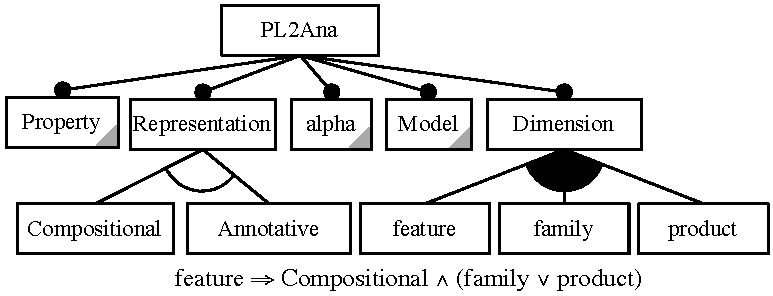
\includegraphics[width = 0.7\linewidth]{figures/fm.pdf}
	\caption{Feature model of the product line of product-line analysis strategies ($PL^{2}Ana$)}
	\label{fig:fm}
\end{figure}
%@TODO lmt: please double check whether "(family or product)" is redundant in the cross-tree constraint.

The feature model shows that $PL^{2}Ana$'s configurability depends on the model and property to be analyzed, on the non-variability analysis function $\alpha$,
on the variability representation (annotative versus compositional), and on dimensions of analysis strategies: feature, family, and product (cf.~\cite{Thum2014}). 
We use the gray triangle in some features to express that we leverage attributes in the feature model to model variability in  property, model, and non-variability analysis function. Attribute values may correspond to the product-line analyses discussed in Section~\ref{sec:strategies} or new analyses on properties allowing an ADD-based representation (cf. Section~\ref{sec:fmkoverview}).  Additionally, the feature model has a cross-tree constraint stating that feature-based analyses require a compositional representation. This way, a configuration of $PL^{2}Ana$ denotes a concrete SPL analysis strategy of a property for a particular model representation.
%specific compositional or annotative representations. 

The asset base comprises foundational elements (types and functions) from which SPL analysis strategies are built as well as their properties. Types refer to models subject to analysis or intermediate analysis results, whereas functions refer to analysis steps. Properties refer to commutative results establishing the soundness of variability-aware 
analyses (cf. Section~\ref{sec:abstraction-description} ). Since the framework targets properties that can be represented in an ADD, as discussed in Section~\ref{sec:fmkoverview}, the functions and types of the lower quadrants of Figure~\ref{fig:strategies-generic}, except \textit{Property}, have the specific interpretation mentioned in Section~\ref{sec:fmkoverview}. However, since we are still interested in an abstract and conceptual description of analyses, the remaining types and functions in $AB$ are either uninterpreted (i.e., we provide no concrete specification nor implementation for them)  or  parameterized, as formalized in Section~\ref{sec:abstraction-description}. For example, the \textit{Product} type is uninterpreted, whereas \textit{Annotative Model} and \textit{Annotative Product Line} are defined directly and indirectly in terms of \textit{Product}, respectively. As additional examples, the $\pi$ function is defined in terms of \textit{Annotative Model} and \textit{Product}; $\alpha$ is uninterpreted, whereas $\hat{\alpha}$ is defined in terms of $\alpha$ and \textit{Annotative Model}.
At a coarse-grained level, all types and functions  must comply with the structure in the diagram. 
%since these also depend on the model and property to be analyzed, \textit{Property}, and $\alpha$ are

The transformational configuration knowledge is responsible for mapping features to transformations over assets. Such transformations are used during product derivation, as explained later in this section. In particular, the model illustrated in Table~\ref{fig:ck} associates feature expressions with type interpretation ($\mathtt{bind}$), partial function application ($\mathtt{select}$), function composition ($\circ$), and function mapping over structure ($\mathit{fmap}$). On the one hand, type interpretation support key concepts in the product-line analysis domain such as $Product$, $Property$, and $\alpha$ to be treated abstractly, thus focusing on its essential concepts and properties, and extending its generality. On the other hand, interpretation needs explicit instantiation, which is a manual step. Partial function application enables selection of the representation of the model to be analyzed: annotative or compositional. The CK additionally uses function composition to combine intermediate analysis steps during product derivation, e.g., 
$\sigma \circ \hat{\alpha}$ combines  the steps of first performing variability-aware analysis ($\hat{\alpha}$) followed by expression evaluation ($\sigma$) when the feature expression $\mathit{annotative} \land \mathit{family} \land \mathit{product}$ in Table~\ref{fig:ck} is satisfied by a configuration. Finally, the CK may also apply analysis steps within a compositional model or expression via $\mathit{fmap}$. For instance, for any configuration of the feature model comprising  the $\mathit{feature}$ feature, the CK applies the variability-aware analysis $\hat{\alpha}$ to all annotative models within the encompassing compositional model.

Additionally, given the cross-tree constraint of the feature model, the compositional representation is also selected, which implies that the type \textit{Compositional Product Line} is instantiated, as specified by the corresponding row in the configuration knowledge. Furthermore, the feature expressions for \textit{Property}, \textit{Model}, and \textit{Representation} evaluate to $\mathtt{true}$, since these are mandatory features, so their corresponding instantiations are always performed. The root feature \textit{PL2Ana} does not appear in the table because it is an abstract feature.



%The transformational configuration knowledge, as stated, is responsible for mapping features into transformations over assets. 
%Since in our case assets are types and functions, the model illustrated in Table~\ref{fig:ck} associates feature expressions with partial function application ($\mathtt{select}$), function composition ($\circ$), and function mapping over structure ($\mathit{fmap}$). 
%Interpretation allows key concepts in the SPL analysis domain such as $Product$,https://www.overleaf.com/project/5dfb7b732691410001bc5ecd $Property$, and $\alpha$ to be treated as parameters of the framework, thus focusing on its essential concepts and properties, and extending its generality. 
%Partial function application enables selection of the concrete model and property to be analyzed, the non-variability aware analysis function, and the representation of the model to be analyzed: annotative or compositional. The CK additionally uses function composition to combine analysis steps, e.g., 
%$\sigma \circ \hat{\alpha}$ combines  the steps of first performing variability-aware analysis ($\hat{\alpha}$) followed by expression evaluation ($\sigma$) when the feature expression $\mathit{annotative} \land \mathit{family} \land \mathit{product}$ holds in Table~\ref{fig:ck}. Finally, the CK  possibly applies these steps in a compositional model or expression ($\mathit{fmap}$). For instance, for a configuration of the feature model comprising both the \textit{feature} and textit{family} features, 
%we compose the corresponding functions in the LHS of Figure~\ref{fig:strategies-generic}. Additionally, given the cross-tree constraint of the feature model, the compositional representation is also selected, which implies that the type \textit{Compositional Product Line} is instantiated, as specified by the corresponding row in the configuration knowledge. Furthermore, the feature expressions for \textit{Property}, \textit{Model}, and \textit{Representation} evaluate to $\mathtt{true}$, since these are mandatory features, so their corresponding instantiations are always performed. The root feature \textit{PL2Ana} does not appear in the table because it is an abstract feature.




%\begin{figure}[t]
%	\centering
%	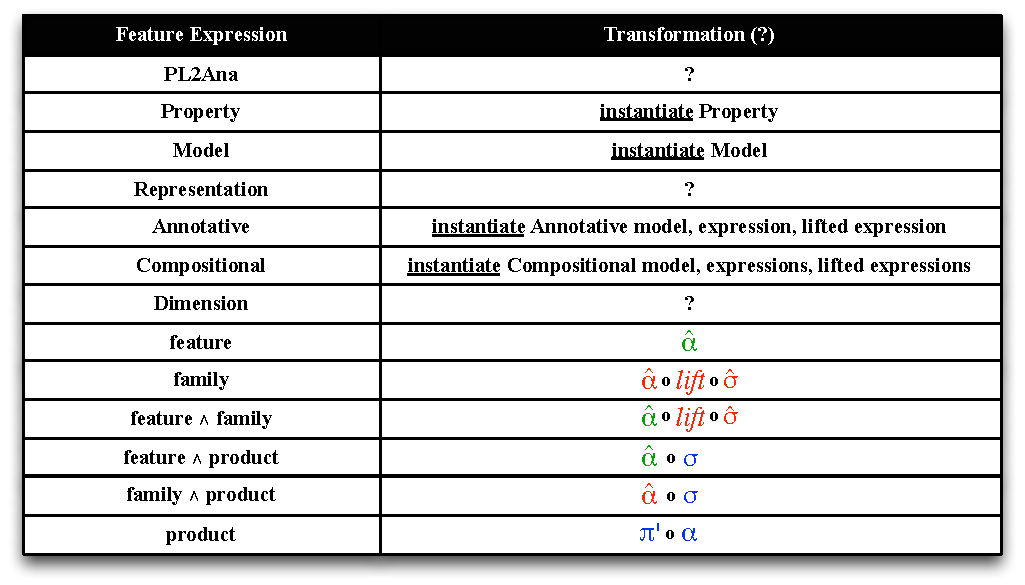
\includegraphics[width = 0.5\linewidth]{figures/ck.pdf}
%	\caption{Configuration Knowledge.}
%	\label{fig:ck}
%\end{figure}

	\begin{table}[htb]
		\centering
		
		\caption{Transformational Configuration Knowledge. Transformation primitives are the functions $\mathtt{bind}$ (type interpretation), $\mathtt{select}$ (partial evaluation), $\circ$ (function composition), and   $\mathit{fmap}$ (mapping over structure). $cModel$ is a compositional model.}
		%\resizebox{\columnwidth}{!}{
			\begin{tabular}{cc}
				\toprule
				
				\textbf{Feature Expression} & \textbf{Transformation} \\\midrule
				$\mathit{Property \mathtt{(true)}}$ & $\mathtt{bind}(\mathit{Property})$  \\
				$\mathit{Model \mathtt{(true)}}$ & $\mathtt{bind}(\mathit{Product})$ \\
				$\mathit{Property} \land \mathit{Model}$     &  $\mathtt{bind}(\mathit{\alpha})$    \\
				%$\mathit{Representation \mathtt{(true)}}$  & $\mathtt{instantiate}(\mathit{Annotative Model})$ \\
				$\mathit{Annotative}$ & $\mathtt{select}(\mathit{Annotative Product Line})$ \\
				$\mathit{Compositional}$  & $\mathtt{select}(\mathit{Compositional Product Line})$ \\    
				$\mathit{annotative} \land \mathit{product}$   &  $  \alpha  \circ \pi  $  \\    
				$\mathit{compositional} \land \mathit{product}$  &  $  \alpha \circ \pi' $  \\    
				%$\mathit{family} \lor \mathit{feature}$  & $\mathtt{instantiate}(\mathit{\hat{\alpha}})$  \\    
				$\mathit{annotative} \land \mathit{family} \land \mathit{product}$ &  $\sigma \circ \hat{\alpha}$  \\    
				$\mathit{annotative} \land \mathit{family}$ &  $\hat{\sigma}  \circ \mathit{lift}   \circ \hat{\alpha} $  \\    
				$\mathit{feature} \land \mathit{product}$  & $  \sigma  \circ \mathit{fmap(\hat{\alpha})} $ \\    
				$\mathit{feature} \land \mathit{family}$  & $ \hat{\sigma} \circ \mathit{fmap(lift)} \circ \mathit{fmap(\hat{\alpha},cModel)}$ \\    
				%$\mathit{product}$    &  $\mathtt{instantiate}(\mathit{\alpha})$    \\    
				\bottomrule
			\end{tabular}
		%}
		\label{fig:ck}
	\end{table}





$PL^{2}Ana$'s products are then product-line analysis strategies for a given model, property, and an originally non-variability-aware analysis technique. Figure~\ref{fig:ad} describes $PL^{2}Ana$'s product derivation process. First, one manually binds--or reuses previously specified--the model, the property to be analyzed, and  the non-variability aware analysis. Following, one decides on the representation (annotative versus compositional). Finally, one chooses the analysis dimensions (feature, family, product). 
Derivation then proceeds by evaluating the $CK$ according to the given configuration, progressively composing the intermediate results of transformations of AB elements corresponding to feature expressions satisfied by the product configuration at hand. Therefore, the resulting product is a specific product-line analysis strategy corresponding to an analysis path in the framework represented in Figure~\ref{fig:strategies-generic}. This product  is build by reuse of AB elements and corresponds to a concrete PVS theory comprising exactly the corresponding analysis function, supporting types, and properties.

% \begin{figure}[t]
% 	\centering
% 	\resizebox{\textwidth}{!}{%
% 	    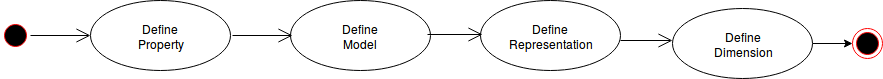
\includegraphics{figures/ad.tikz}
%     }
% 	\caption{Product Derivation Workflow}
% 	\label{fig:ad}
% \end{figure}
% %@TODO: update figure to insert taks "Define alpha (non-variability analysis) after "Define Model"

\begin{figure}[t]
	\centering
	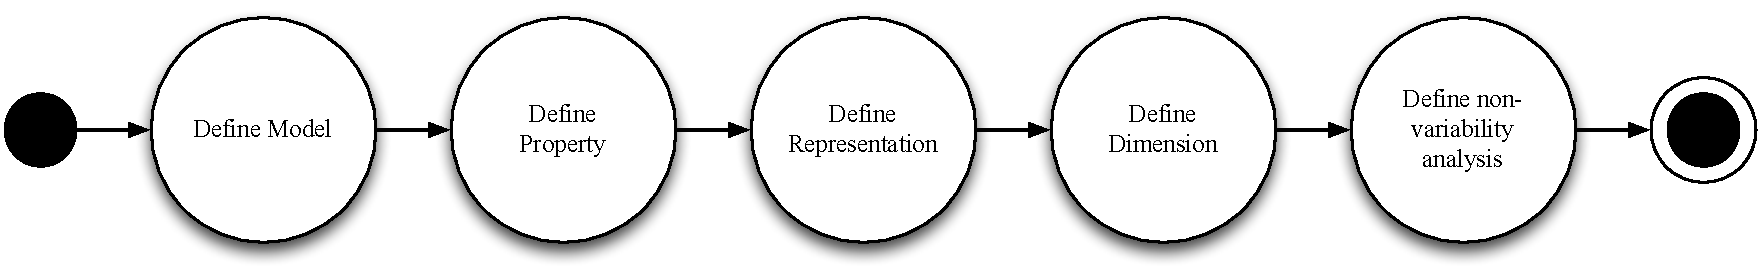
\includegraphics[width = 0.9\linewidth]{figures/workflow.pdf}
	\caption{$PL^{2}Ana$'s product derivation process}
	\label{fig:ad}
\end{figure}

An example of $PL^{2}Ana$'s product derivation process is given in Figure~\ref{fig:workflow-reliability}. 
We see that we might derive a family-product reliability analysis for annotative models 
by binding property and model attributes as Reliability and DTMC, respectively. 
Moreover, we select the representation and analysis dimension accordingly, 
to produce an analysis strategy that corresponds to the top-right quadrant of Figure~\ref{fig:strategies-generic}, 
particularly instantiated with the chosen property and model. 

\begin{figure}[htbp]
	\centering
	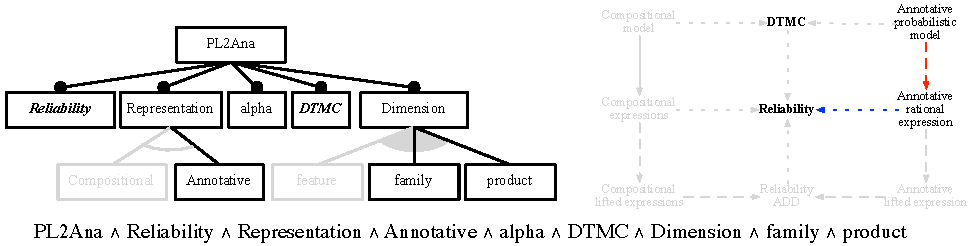
\includegraphics[width=0.9\linewidth]{figures/workflow-reliability.pdf}
	\caption{Example of $PL^{2}Ana$'s product derivation process with reliability analysis}
	\label{fig:workflow-reliability}
\end{figure}

Another example of $PL^{2}Ana$'s product derivation process is given in Figure~\ref{fig:workflow-behavior}. In this example, we derive a feature-family behavior analysis for compositional models (SMV and fSMV)
by choosing CTL and TS as property and model attributes, respectively. 
Moreover, we select the representation and analysis dimension accordingly, 
to produce an analysis strategy that corresponds to the LHS of Figure~\ref{fig:strategies-generic}, 
particularly instantiated with the chosen property and model. We note that this instance extends the scope of the state-of-the-art of product-line behavior analyses represented in Figure~\ref{fig:diagram-FTS}, thereby providing evidence that the configurability of our framework allows exploring novel analyses.

\begin{figure}[htbp]
	\centering
	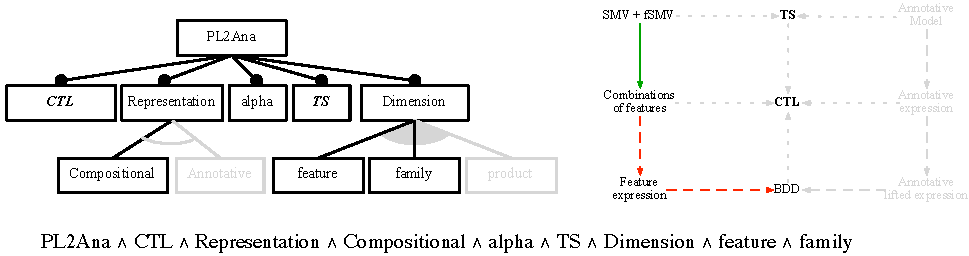
\includegraphics[width=0.9\linewidth]{figures/workflow-behavior.pdf}
	\caption{Example of $PL^{2}Ana$'s product derivation process with behavioral analysis}
	\label{fig:workflow-behavior}
\end{figure}


%vra: I think we should consider dropping this section, since it looks outside the main focus
%\subsection{Evolution of Product Line of Product-Line Analyses}
%\label{sec:evolpl2ana}
%In Section~\ref{sec:abstraction-description}, we addressed the generalization of the the analyses represented in Figure~\ref{fig:strategies-overview}. Essentially, we abstracted fundamental concepts (property, model, non-variability-aware analysis) into uninterpreted types and dependent concepts into parametrized types and functions  with assumptions along the structure of the diagram. In this section, we describe the development of product lines of product-line analyses in terms of a principled evolution of previous works. Such evolution can be useful for further safe evolution of the proposed framework.

%Motivated by the need to empirically compare the proposed feature-family reliability analysis strategy to other strategies, \citet{LANNA2017} implemented the ReAna tool, which actually realizes the diagram in Figure~\ref{fig:strategies-overview}. 
%As depicted in Figure~\ref{fig:evol}, such evolution can be safely described by applying  the \textit{merge template}~\cite{NevesBATTSK15} to incrementally evolve the product line, starting from the feature-family-based~\cite{LANNA2017} and feature-product-based strategies~\cite{Ghezzi2013}, then incorporating the family-product-based~\cite{nunes_variability_2012} and lastly the family-based~\cite{FDTMC}  strategies. The process' soundness  follows from the soundness of the employed template. 

%\begin{figure}[t]
%	\centering
%	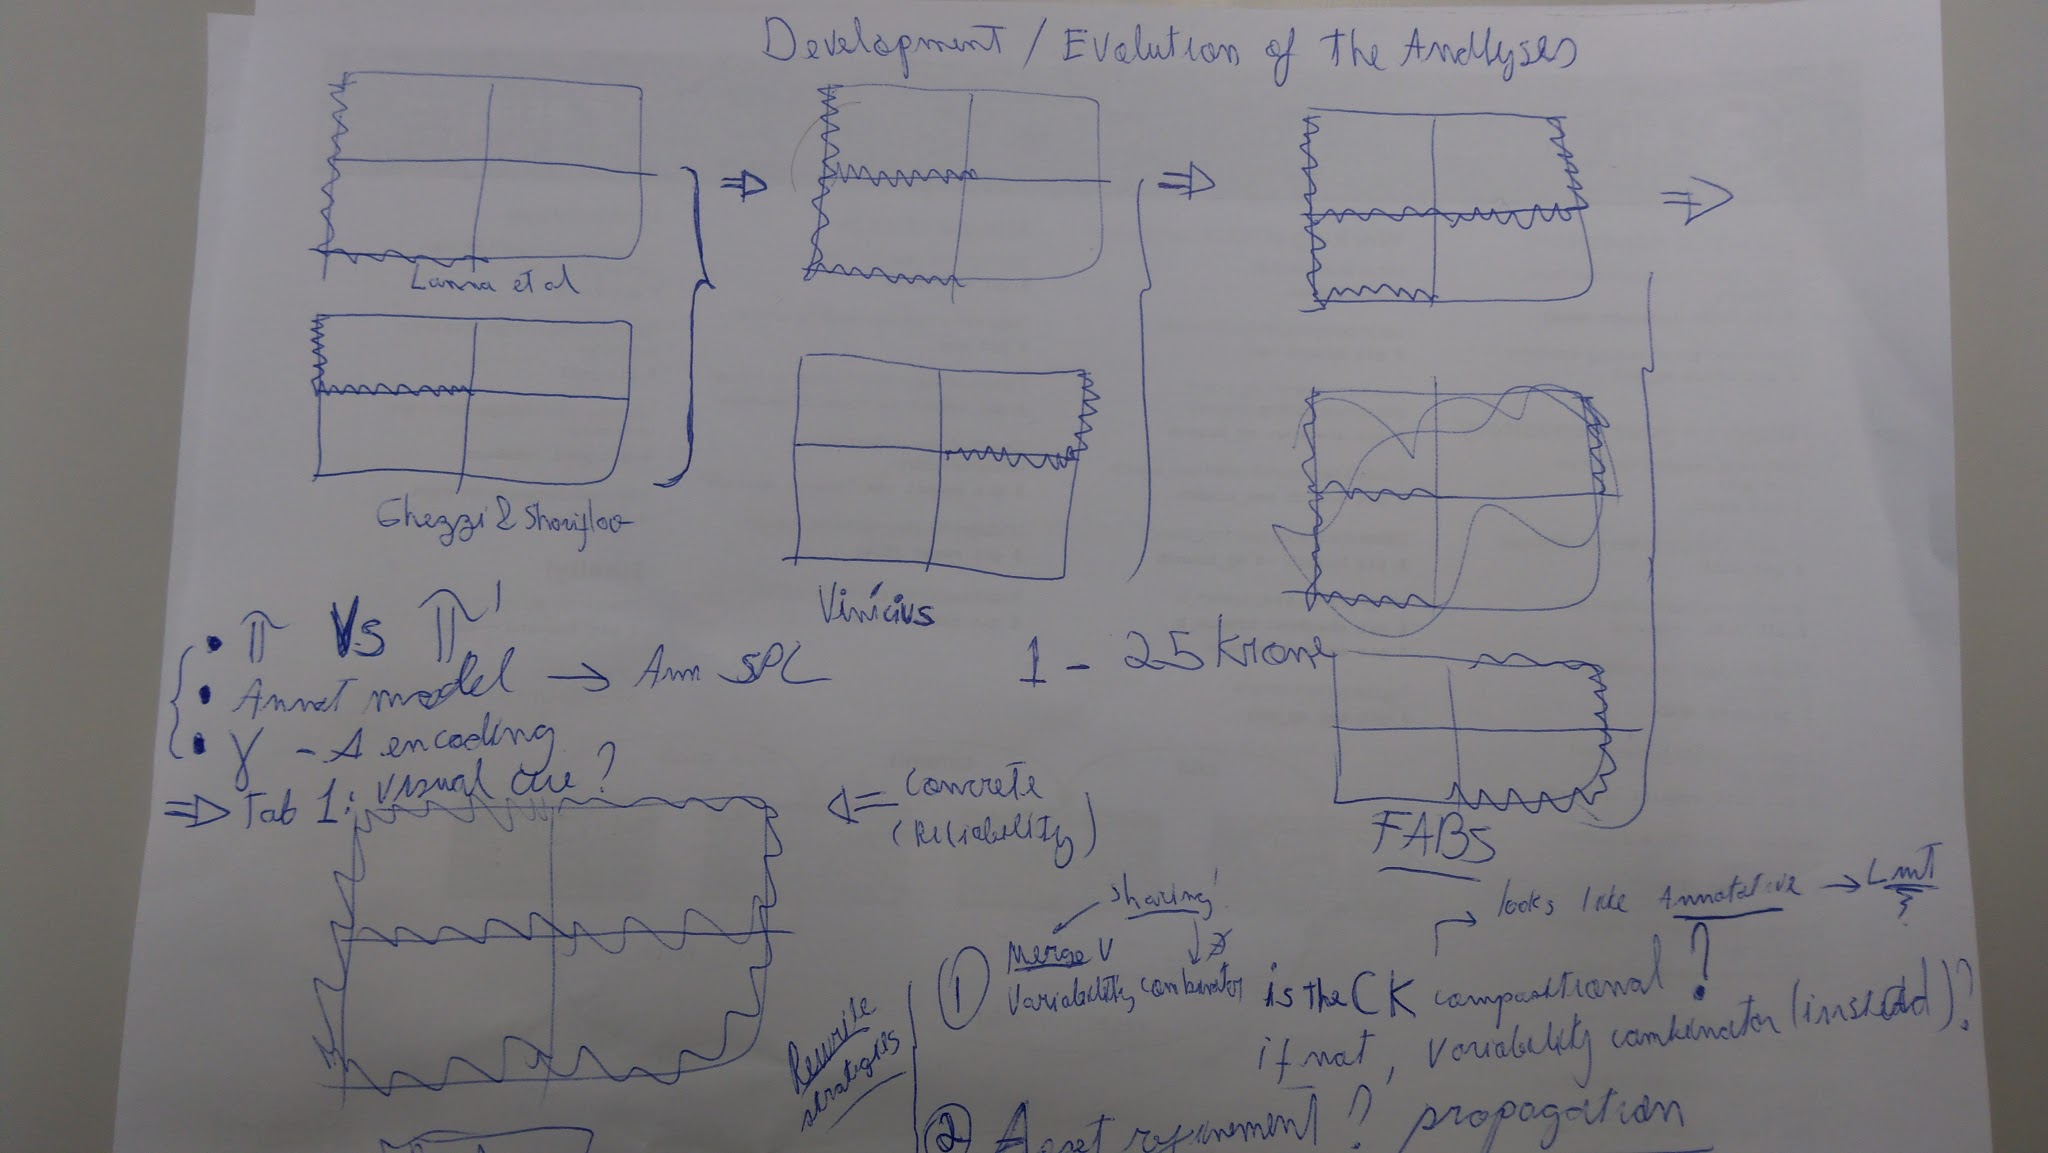
\includegraphics[width = 0.9\linewidth]{figures/evol.jpg}
%	\caption{Evolution of Product Line of Product-Line Reliability Analysis Strategies.}
%	\label{fig:evol}
%\end{figure}




\section{Discussion}
\label{sec:evaluation}
The formalization described in Section~\ref{sec:abstraction-description}, which as mechanized into PVS, provides formal evidence on the validity of the framework. In this section, we complementarily evaluate the framework qualitatively. 
%Correspondingly, 
We first discuss the framework's generality (Section~\ref{sec:frameworkInstances}). Then, we discuss findings, related strengths, and limitations (Section~\ref{framework:discussion}). Finally, we discuss threats to validity  (Section~\ref{sec:threatsToValidity}).

\subsection{Framework's Generality}
\label{sec:frameworkInstances}

%To qualitatively assess the generality of the framework, we retrospectively discuss to what extent it can describe five representative product-line analyses~\cite{Thum2014} on the following properties: safety, performance, inter-procedural static analyses, security, and functional program properties. 
In this section, we qualitatively assess the framework's generality by retrospectively discussing to what extent it can describe existing product-line analyses. In particular, we show how  the framework's elements, previously listed in Table~\ref{table:analysis-abstraction-framework} and within the structure of the generic diagram in Figure~\ref{fig:strategies-generic}, can be related to different models, properties, and analyses. 
%The first column in Table~\ref{fig:inst} refers to framework's elements, whereas the remaining columns correspond to product-line analyses proposed elsewhere. 
These analyses were chosen because three of them (safety, data-flow facts, and functional program properties) represent different types in a comprehensive survey~\citep{Thum2014} and  the remaining two (performance and security) are more recent. 
%we conceptually discuss instances of the framework thereby qualitatively assessing its generality. 
An analytical assessment, by instantiating the mechanized theory (cf. Section~\ref{sec:abstraction-description}) for concrete analyses, is yet to be performed. Such task is outside the scope of this work and is regarded as future work. 

%In every cell from the second column onwards, we refer to the counterpart of the framework's element in each work by mentioning the corresponding concrete concepts therein together with definition numbers when available. In the following sections, we discuss each analysis.

%In this section, we conceptually discuss instances of the framework thereby qualitatively assessing its generality. Mechanized instantiation in PVS is outside the scope of this work and is regarded as future work. 
%Table~\ref{fig:inst} synthesizes this assessment, showing how  the framework's elements, previously listed in Table~\ref{table:analysis-abstraction-framework} and within the structure of the generic diagram in Figure~\ref{fig:strategies-generic}, can be instantiated for different models, properties, and analyses. 
%The first column in Table~\ref{fig:inst} refers to framework's elements, whereas the remaining columns correspond to product-line analyses proposed elsewhere. These analyses were chosen because they represent different types  in a comprehensive survey~\citep{Thum2014} and the last one is more recent. In every cell from the second column onwards, we refer to the instantiation of the framework's elements in each work by mentioning the corresponding concrete concepts therein together with definition numbers when available. In the following sections, we discuss each instance.


\subsubsection{Safety Analysis}
\label{sec:instance-splverifier}

\citet{ApelSimulator} provide the toolchain SPLverifier for empirically comparing family-based, 
product-based, and sample-based model checking of domain-specific safety properties in product lines 
written in C and Java. To manage variability, the authors leverage a compositional representation, using 
feature modules and derivation via superimposition~\cite{FeatureHouse}. For product-based analysis, all 
products corresponding to valid configurations are derived via superimposition and then model-checked 
against a number of safety properties via explicit-state model checking. The sample-based analysis is an 
optimized version of product-based analysis, whereby different strategies are used: 1-wise, 2-wise, and 
3-wise, each of which defines a corresponding sampling function for selecting subsets of products to be 
model-checked, after which the analysis is product-based.  

In contrast, for family-based analysis, first the composition mechanism of FeatureHouse~\cite{FeatureHouse} is adjusted to 
perform variability encoding: essentially, the variability induced by different combinations of features 
is encoded in the form of conditional program executions using if statements so that the product line is 
transformed into a product simulator, which simulates the behavior of all products,
depending on the values of feature variables that represent the presence or absence of individual features. 
Then, off-the-shelf model checkers are used to perform verification of safety properties by means of explicit-state 
and symbolic model checking. The model checker exploits sharing between products using two principles: late 
splitting and early joining. The former means performing analysis without variability until encountering it, 
that is, the model checker explores execution paths of different products only once as long as such paths are 
equal; the latter means attempting to join intermediate results as early as possible, so analysis branches 
differing only on the value of feature variables should be analyzed only once. The result of model checking 
are sets of products, which are encoded in BDDs for efficient representation.

\begin{figure}[!htbp]
	\centering
    %\resizebox{\textwidth}{!}
	\caption{Framework description of  the work by \citet{ApelSimulator} (\Cref{sec:instance-splverifier})}
	\label{fig:instance-splverifier}
\end{figure}

\subsubsection{Performance Analysis}
\label{sec:instance-performance}

\citet{kowal_scaling_2015} present an approach for variability-aware analysis of software performance 
models. The underlying variability-free model is a Performance Annotated Activity Diagram (PAAD), which is an UML 
activity diagram with performance annotations. In such a model, nodes represent a service center with given multiplicity, 
initial client distribution, and service time distribution; edges are annotated with probabilities to model operational 
profiles. Based on this model, the property of interest is throughput, which is defined as the difference between the 
number of incoming and outcoming jobs out of all service stations of the model. The non-variability-aware analysis of 
this PAAD abstracts this model as a Markov population process and approximates its behavior by a compact system of 
ordinary differential equations (traffic equations), whose solution is the throughput of the model. 

Variability management is accomplished via delta-modeling such that a core PAAD is represented together with a set 
of deltas adding, removing, or modifying vertices and edges (compositional representation). A variant can be obtained 
by applying such deltas and then the previous variability-free analysis can be applied. Alternatively, variability 
encoding of deltas transforms the compositional model into a 150\% model (annotative representation), which subsumes every concrete variant of the family, consisting of all nodes and transitions that are 
added or modified by some delta.
This model undergoes variability-aware analysis, whereby a parametric\footnotemark{} system of ordinary differential equations 
is solved, giving rise to an algebraic expression.
Such expression is then evaluated for each possible configuration, yielding a family-product-based analysis.
Similar to Classen et al. for model checking, Kowal et al. have not explored compositional (feature-based) reasoning.
\footnotetext{All elements that are added to, removed from, or modified in the 150\% model are represented by parameters.}

\begin{figure}[!htbp]
	\centering
    %\resizebox{\textwidth}{!}
	\caption{Framework description of the work by \citet{kowal_scaling_2015} (\Cref{sec:instance-performance})}
	\label{fig:instance-performance}
\end{figure}

%The work of Kowal et al.~\cite{kowal_scaling_2015} presents a formalism to describe performance models of product lines based on performance-annotated activity diagrams (PAAD) described in a delta-oriented language.  The semantics of their models is expressed by continuous-time Markov chains (CTMC), which are more appropriate to performance analysis than DTMCs. They perform family-product based throughput analysis of a model derived from the delta modules.  Accordingly, they first apply variability encoding to delta PAAD deltas to obtain a 150\%model (annotative representation). Next, they analyze this model by means of symbolic linear equation solving, and then perform expression evaluation. 




%To provide evidence of the framework's generality, we show in Table~\ref{fig:inst}
%how its elements, previously listed in Table~\ref{table:analysis-abstraction-framework} and within the structure of the generic diagram in Figure~\ref{fig:strategies-generic}, can be instantiated for different properties and existing analyses. Each column in Table~\ref{fig:inst} describes a group of analysis strategies 
%for some model and property. The first column refers to framework's elements, whereas the remaining columns 
%correspond to analysis strategies proposed elsewhere, which we briefly describe next. In every cell from the second column onwards, we refer to the instantiation of the framework's elements in each work by mentioning the corresponding concrete concepts 
%therein together with definition numbers when available.


\subsubsection{Security Analysis}
\label{sec:instance-security}

\citet{securityGPCE18} contribute SecPL, a method for managing security requirements systematically in an SPL, promoting model-based security analysis. SecPL extends UML's security profile UMLsec supporting the specification of security requirements and annotative variability in UML models with presence conditions. Users leverage UMLsec stereotypes for encoding security specifications as OCL constraints. Such specifications can be done manually  or automatically mined from annotated source code. The authors rely on \textit{template interpretation}~\citep{templateInterpretation} to perform a family-based approach, lifting checks such as secure dependencies from the level of individual products to the entire SPL. Accordingly, OCL constraints comprising the security property specification are analyzed on the annotative UML model, resulting in a feature expression, which is checked for satisfiability. If the formula is satisfiable, the feature set generates an unsafe product. Otherwise, one has a proof that each product satisfies the specified security properties.

\begin{figure}[!htbp]
	\centering
    %\resizebox{\textwidth}{!}
	\caption{Framework description of the work by \citet{securityGPCE18} (\Cref{sec:instance-security})}
	\label{fig:instance-security}
\end{figure}

\subsubsection{Data-flow Analysis}
\label{sec:instance-spllift}

The generalization of the structure of our diagram is  not limited to the verification of 
probabilistic and non-probabilistic behavioral properties. Consider, e.g., the variability-aware static analysis method proposed by~\citet{SPLLift}. Their method, named SPL$^{LIFT}$, seamlessly 
lifts inter-procedural data-flow analysis to product lines. To that end, they annotate an inter-procedural control-flow graph with a feature or its negation, to represent the cases where the feature is enabled or not, 
respectively. The variability-aware analysis then maps features expressions describing the configuration space of the annotated control-flow graph to corresponding data-flow facts.
%This leads to parametric data-flow functions which can be composed to represent the flow of 
%all the product-line products in a concise representation. 
This representation is similar to the annotative FTS 
models introduced by \citet{Classen2013} for behavioral model checking. 
The generalization of the structure of the diagram is therefore also similar: from the annotated inter-procedural control-flow graph, 
one can perform a family-based analysis and find the set of products leading to a violation. 
This set can be compactly encoded as a constraint over the features, which is equivalent to a feature 
expression. As \citet{Classen2013} for model checking, \citet{SPLLift} have not explored compositional 
(feature-based) reasoning.

\begin{figure}[!htbp]
	\centering
    %\resizebox{\textwidth}{!}
	\caption{Framework description of the work by \citet{SPLLift} (\Cref{sec:instance-spllift})}
	\label{fig:instance-spllift}
\end{figure}

%\begin{landscape}
%	\begin{table}[htb]
%		\centering
%		
%		\caption{Generality of the analysis framework}
%		\resizebox{\columnwidth}{!}{
%			\begin{tabular}{llllll}
%				\toprule
%				
%\textbf{Framework element} & \textbf{\citet{ApelSimulator}} & \textbf{\citet{DOPTheo}}  & %\textbf{\citet{kowal_scaling_2015}} & \textbf{\citet{SPLLift}} & \textbf{\citet{securityGPCE18}}  \\\midrule
%Property & Safety & Functional program properties & Throughput  & inter-procedural static analyses & Security\\
%Product & Java and C code & Abstract Behavioral Specification & PAAD (Def. 1) & Control-flow graph & UMLSec \\
%Compositional Product Line & Feature modules & ABS core and deltas & PAAD and PAAD deltas (Def. 5) & -- & -- \\    
%Annotative Product Line & \textit{if} statements & -- & 150\% model (Def. 7) & Annotated flow functions & SecPL\\
%Compositional expressions & -- & -- & -- & -- & -- \\    
%Annotative expression & Feature expression & -- &  Parametric traffic equation & Feature expression & Feature expression \\    
%Compositional lifted expression & -- & -- & -- & -- & --\\    
%Annotative lifted expression & Lifted feature expression & -- & -- & Lifted feature expressions & --\\    
%Property ADD & BDD & -- & -- & BDD & -- \\    
%Projection  & -- & -- & Projection (Def. 8) & Propagation & Projection \\    
%Composition & Superimposition & Delta application & PAAD delta application (Def. 6) & -- & -- \\     
%Analysis  & Model checking & Theorem proving & Traffic equation solving (Def. 4) & IFDS analysis & OCL check \\     
%Variability-aware analysis & Model checking & Theorem Proving &  Parametric traffic equation solving & IFDS/IDE analysis & template interpretation+SAT \\     
%Evaluation & -- & -- & Expression evaluation & -- & Expression evaluation \\     
%Evaluation with ADDs  & BDD evaluation & --  & -- & BDD evaluation & --  \\     
%\textit{lift} & \textit{lift} & -- & -- & \textit{lift} & -- \\     
%Variability encoding & Variability encoding & -- & Variability encoding & -- & --\\     
%ADD application & BDD application & -- & -- & BDD application & --\\ 
				
%				\bottomrule
%			\end{tabular}
%		}
%		\label{fig:inst}
%	\end{table}
%\end{landscape}



\subsubsection{Functional Program Properties Analysis}
\label{sec:instance-delta-liskov}

\citet{DOPTheo} present a feature-family-based analysis strategy for product lines based on Delta Oriented 
Programming (DOP) to analyze functional program properties expressed as contracts and invariants. Programs are expressed as a core and a number of delta modules that add, remove, or modify methods, 
fields, and contracts. To guarantee uniqueness of variant derivation for a given set of deltas, it is assumed that 
a partial order exists between the deltas. Program derivation proceeds by composing the core with a sequence of deltas. 

The analysis proposed by \citet{DOPTheo} relies on an extended Liskov principle for DOP, whereby the method contracts of subsequent deltas 
must become more specific; invariants cannot be removed, but only added; methods called in deltas use the 
contract of the first implementation of that method.
Leveraging such constraints, the core and each delta are analyzed in isolation 
with respect to method preconditions and postconditions (feature-based phase).
After that, the global program invariants in the core and deltas are combined and
checked (family-based phase), considering that method contracts are the ones
computed in the previous step.

The resulting process can be seen as a feature-family-based verification
approach for delta-oriented product lines~\cite{Thum2014}.
However, the analysis technique proposed by \citet{DOPTheo} results in a yes/no
answer to the question of whether all possible applications of deltas yield
products that satisfy their corresponding specifications.
This means that intermediate results can neither be represented as expressions nor
lifted to ADD semantics.
Hence, that approach cannot be described by our proposed framework.




\subsection{Higher-level Abstractions}

\label{framework:discussion}

In addition to the generality discussed in the previous section, our framework also has higher-level abstractions comprising a number of its elements. Identifying these abstractions  contributes to improving a principled understanding of product-line analyses. These abstractions are the following:

\begin{itemize}

    \item \textbf{\textit{Inwards}---Variability binding}: From  either side of Figure~\ref{fig:strategies-generic} to its center, there is variability restriction, which binds the variability according to a configuration. Such step is performed at different types (models and expressions) and granularity levels (annotative and compositional models and expressions).	
    For example, $\pi'$ binds variability in compositional models, whereas $\pi$ binds variability in annotative models.

	\item \textbf{\textit{Left side}---Component functor}: Within the leftmost models in Figure~\ref{fig:strategies-generic}, there is a functor (a structure that can be mapped over) capturing the structure of the compositional model across compositional expressions and lifted compositional expressions (cf. dotted arrows in Figure~\ref{fig:functor}). The $\mathit{fmap}$ function maps the variability-aware analysis function $\hat{\alpha}$ over this structure of compositional model 
	(cf. edge labeled $\mathit{fmap(\hat{\alpha})}$ in \Cref{fig:strategies-generic} and first large horizontal arrow in Figure~\ref{fig:functor}), yielding a corresponding compositional expression. A further call to \textit{fmap} maps the \textit{lift} function over this expression ($\mathit{fmap(lift)}$), resulting in a lifted compositional expression. 
	
	
	\item \textbf{\textit{Left side}---Folding functor with partial composition}:
	Additionally, from the left-hand side to the center, the variability binding step is performed within a folding operation over an ordering of the component functor structure to obtain a product ($\pi'$) or a property value 
	($\sigma$ and $\hat{\sigma}$). The folding implies the existence of both \pvscode{partialModelComposition} and \pvscode{partialExpComposition}, which bind the composition mechanism for \pvscode{AnnotativeModel} and \pvscode{AnnotativeExpression}, respectively. 
	%Further, annotative models and expressions are homomorphic via the $\mathit{\hat{\alpha}}$. This encodes the compositional assumption on the analysis.
	%The folding implies the existence of an associative composition operation on annotative models and expressions as well as the existence of an identity element. Therefore, annotative models and expressions  are \textit{monoids}. 
	%Further, these monoids are homomorphic via the $\mathit{\hat{\alpha}}$. This encodes the compositional assumption on the analysis.
	
		%	\item \textbf{Variability- and non-variability aware analyses}: If we assume that the \textit{Annotative Model} is hierarchical (or perhaps by a weaker restriction, that the model's elements are related via a well-founded relation), then we could relate such analyses in a more explicit way: the variability-aware analysis amounts to following the hierarchical structure and at each level applying the non-variability aware analysis in the common fragment of the model at that level in the hierarchy while evaluating the resulting expression with the recursive application on the variant branches;
	%	
	\item \textbf{\textit{Lower quadrants}---Lifting to ADDs}: Both lower quadrants of the diagram in Figure~\ref{fig:strategies-generic} illustrate a general principle for lifting analyses to product lines using ADDs: the intermediate analysis results represented by either compositional or annotative expressions are encoded using ADD operations for concise representation and obviating from enumeration during algebraic manipulation and evaluation. Further details can be checked elsewhere~\cite{Castro2017}.
\end{itemize}


\begin{figure}[htb]
	\centering
    \resizebox{\textwidth}{!}{%
        \includegraphics{figures/component-functor.tikz}
    }
	\caption{Component Functor, allowing structure-preserving transformations}
	\label{fig:functor}
\end{figure}

Regarding generality (cf. Section~\ref{sec:frameworkInstances}), we note that product-line analyses for both functional and non-functional properties can be described. In general, depending on 
the property and model, the total number of possible analysis strategies may change. Although for reliability~\citet{Castro2017} formalize seven analyses, this does not necessarily hold for all other properties, since some of these  may not be
amenable to compositional reasoning (e.g., performance). 
%Indeed, the diagram itself is \textit{configurable}. 
Additionally, in principle, new analyses can also be conceived based on the original diagram. 
For instance, the performance analysis by \citet{kowal_scaling_2015} results in algebraic expressions, which, in principle, could be subject to lifting and ADD-based evaluation.
New analyses could also arise for other models and properties. As another example, the behavioral analyses described in \Cref{fig:diagram-FTS} could be extended along the compositional dimension of the framework.

At a finer grain, the extent to which our framework supports reuse depends on the property and on the model at hand. For instance, for reachability properties, the same model (PMC) for reliability can be reused. By analyzing the source code of the ReAna tool~\cite{LANNA2017}, we note that it is possible to achieve high level of reuse of both conceptual and implementation aspects. Similar considerations apply for other probabilistic properties. However, in other cases, the overall structure of the analyses could still be reused. For instance, in the product-based case, there is enumeration on products. In the family-based strategies, the common part of the model is explored until variation points branch out the analysis. In feature-based analysis, each model fragment related to a feature is analyzed. This overall control can be abstracted and shared across different properties and models thus helping the development of new analysis strategies.

Accordingly, the formalization carried out in Section~\ref{sec:abstraction-description} supports reuse by focusing on key abstractions and properties in this domain. 
In terms of abstractions, reuse follows from types and functions defined directly or indirectly in terms of the framework's core concepts, i.e, the property, the model, and the corresponding non-variability-aware analysis.
%In particular, this amounts to five types and four functions defined from the three parameters, plus three types and four functions reused across all analysis (lower quadrants).  
Regarding properties, the framework  also supports reuse of commutative properties, which are essential for the soundness of product line analysis strategies, but are usually a non-trivial and scarce effort across independently developed analyses. As discussed in Section~\ref{sec:abstraction-description}, proofs of commutative properties of our framework are a high-level structure that is completely reused under different interpretations for different models and  related properties. Moreover, proof reuse is also possible within the framework: the proof of the commutativity of Figure~\ref{fig:strategies-generic}'s  upper-left quadrant  reuses the proof of its upper-right quadrant's  commutativity. Essentially, this means that the soundness of compositional analyses, which are coarse-grained, rely on the soundness of standard analyses, which are finer-grained and non-necessarily compositional. Nevertheless,  the commutativity proof of Figure~\ref{fig:strategies-generic}'s  upper-left quadrant has the liability of an underlying proof obligation corresponding to~\Cref{axiom:compositionality-hat-alpha} %Axiom \lstinline[mathescape=true]{hatAlphaCompositionality} 
in Section~\ref{sec:abstraction-description} requiring basic compositional behavior of the model and its partial composition, which is model dependent. This way, by also explicitly stating the abstract requirements that a model and related transformations must satisfy, the framework supports reuse.

Finally, although the commutative diagram in Figure~\ref{fig:strategies-generic} shows logically equivalent analyses for a given model and property, the diagram
does not convey practical considerations in terms of efficiency. For instance,  
for the feature-product-based analysis to be efficient, it is necessary that recursive composition of expressions is less complex than building the whole product~\cite{Ghezzi2013}. Otherwise, the product-based analysis is preferable. 
In general, such considerations may also depend on modeling pragmatics and could be used to define modeling styles and 
corresponding bad smells.
Furthermore, for a given property and model, the alternative strategies have differing complexity costs, which could 
annotate the diagram, yielding another dimension. A still open question is whether these costs can be reused across 
properties or models~\cite{LANNA2017,StaticAnalysisInPractice,TypeCheckingComparison,SamplingStrategies}.



\subsection{Threats to Validity}
   \label{sec:threatsToValidity}
Our formal framework was inductively built from different product-line analysis
strategies (cf. \Cref{sec:strategies}) and is based on the taxonomy proposed by
\citet{Thum2014} and on the product-line representation by \citet{Kastner2008}, which have been used to describe and analyze a plethora of product lines~\cite{Thum2014}.
Nonetheless, the analysis strategies we considered in \Cref{sec:strategies}  operate over transition-system models (either
DTMC~\cite{LANNA2017,Castro2017} or FTS~\cite{Classen2013,Classen2014}), which brings
the risk of overfitting.
To mitigate that risk, we qualitatively assessed the framework under additional
strategies, operating over transition systems (CTMC~\cite{kowal_scaling_2015}), source
code~\cite{ApelSimulator,SPLLift}, UML models~\cite{securityGPCE18}, and formal
artifacts~\cite{DOPTheo}.
We argue that such variety of analyzed models is a representative sample from the
universe of product-line analysis techniques surveyed by \citet{Thum2014}.
Moreover, a recent survey on the state-of-practice of
variability-aware static analyses in different application domains
\cite{IndustrialAnalysisSurvey} found that reliability,
correctness, and performance are critical properties of interest.

Furthermore, considering the generality assessment  in Section~\ref{sec:frameworkInstances}, we see that the
lower quadrants of our commuting diagram are somewhat misrepresented in the
qualitative assessment.
This raises the question of whether lifting to ADDs can actually be generalized to
other analyses.
Indeed, the proposition of ADD lifting as a technique to cope with product-line
analysis is recent~\cite{LANNA2017}, so there are still no additional empirical
studies that employ it.
Nonetheless, we have analytical evidence that such technique can be employed to
analyze any propoerty that can be expressed as an algebraic
expression~\cite{Castro2017}.

Besides human scrutiny, we further increase the evidence on the soundness of our
commutativity framework by means of machine-based verification.
To address the validity of the mapping between framework concepts and formal
definitions, we created our mechanized theory by modeling the constructs
that exist in the formal theory of commuting product-line reliability analysis
strategies~\cite{Castro2017}.
However, it is future work to assess the extent to which one can devise mechanized
theories of concrete analysis strategies by instantiating our generic PVS theory.
\section{Related Work}
\label{sec:relatedWork}

\paragraph{Conceptual models and taxonomy:}
\citet{Thum2014} established the taxonomy for product-line analyses upon which we based our work, that is, the classification
of analysis techniques in three basic strategies (product-based, feature-based, and family-based) and combinations thereof.
Furthermore, \citet{AnalysisToolsSurvey} surveyed existing product-line analysis tools and categorized them along four criteria:
product-line implementation technique (annotation-based \textit{versus} composition-based approach),
analysis technique (e.g., testing, type checking, model checking),
strategies for product-line analysis (i.e., the analysis strategies taxonomy by \citet{Thum2014}),
and strategy of the tool (product-based, variability-aware, and variability-encoding).
In this work, we build upon these existing taxonomies to propose a framework relating
analysis \emph{steps} in all dimensions.
Moreover, although the surveys by \citet{Thum2014} and \citet{AnalysisToolsSurvey}
range over a larger amount of primary studies, our work establishes finer-grained
relationships between analysis steps, supported by formal reasoning.
In principle, our framework could be applied to describe the studies surveyed by
\citet{Thum2014} and \citet{AnalysisToolsSurvey}---for instance,
the ones that are part of the qualitative analysis in
\Cref{sec:instance-splverifier,sec:instance-spllift}.

\citet{PLAModel} proposed the PLA model, which the authors argue is a
formal model for describing and comparing product-line analyses.
That model consists of four operators that express possible manipulations
of product line artifacts during analysis.
Our commuting diagram  (\Cref{fig:strategies-generic}) relates  to the PLA model as follows:
all downward arrows are instances of \emph{processing step},
all straight arrows from either left or right to the center are instances of \emph{variability restriction}, and
all arcs from left to right are instances of \emph{variability combinator}.
Moreover, whereas \citet{PLAModel} provide static building blocks for
describing product line analyses, we present structurally related
analysis steps and formalize conditions for their applicability.

\citet{SPLAnalysisTime} discussed the analysis of product lines throughout their
life cycle.
The authors reviewed product-line analysis techniques that can be applied to
regression analysis and, conversely, revision analyses that can be leveraged in a
space-variant setting.
Then, \citet{SPLAnalysisTime} conjectured that analyses of product-line variations
in time (i.e., evolution) could be modeled as a fourth dimension in the PLA
model~\cite{PLAModel}, combining both types of techniques.
Within the scope of such modeling effort, we envision that our work can be
extended to cover the time dimension as well, leveraging the finer-grained (yet generic) analysis steps.

% existing formalization x we generalize and identify key concepts and assumptions
\paragraph{Formal approaches to variability-aware analysis:}
The definition of product-line analysis techniques that are sound by construction has been investigated
recently~\cite{Midtgaard2015,ErwigAnalysis,Intraprocedural} in different contexts.
\citet{Midtgaard2015} presented a methodology to systematically derive family-based static analyses from single-product analyses
based on \emph{abstract interpretation};
\citet{ErwigAnalysis} defined a framework for automatic lifting of
static analyses that are expressible as type systems;
and \citet{Intraprocedural} proposed a
technique to automatically lift \emph{intraprocedural data-flow analyses} to handle
variability in product lines.
In contrast to their work, we provide a basis for structuring proofs of correctness
without constraining them to a specific analysis technique formalism.
On the other hand, we expect users of our framework to perform more formalization
activities to bridge their concrete setting to our abstract one.
Moreover, whereas \citet{Midtgaard2015}, \citet{ErwigAnalysis}, and
\citet{Intraprocedural} handle only the family-based
dimension of analysis,
we also address the feature-based dimension.

%\citet{StaticAnalysisInPractice} focus on the practical aspects of static analysis by implementing variability-aware control-flow and data-flow analyses for highly configurable systems, based on the \textsc{TypeChef} tooling infrastructure. Their evaluation shows that the work scales to real-world systems and the performance is comparable to that of sampling techniques. They focus on the family-based dimension and employ sharing techniques to leverage existing analyses in the variability context.

Through their seminal work on FTS, Classen et al. \cite{Classen2013,Classen2014} laid the foundations for designing product-line model checking strategies.
\citet{Classen2013} were concerned with annotative strategies (i.e., the right-hand side of our framework diagram). The principles of their strategies were later reused and extended to solve automata-based verification problems (e.g. real-time model checking \cite{Cordy2013}, 2-player games \cite{Greenyer2013b}).
\citet{Classen2014} proved the equivalence between compositional and annotative FTS (i.e., the existence of the encoding function $\gamma$ for these models). Our framework highlights that purely compositional strategies (i.e., the left-hand side of our diagram) have not been investigated for FTS.

Earlier work on product-line model checking \cite{Fantechi2008} represents the behaviour of multiple products as modal automata, i.e., automata with optional and mandatory transitions. While such modeling allows checking that given properties hold for the whole product line, they cannot trace back the features responsible for property violations. Framing this verification problem within our framework would indeed highlight the impossibility to construct annotative (lifted) expressions. This limitation was later circumvented by extending modal automata with variability constraints \cite{Asirelli2011,TerBeek2016}. This makes modal automata as expressive as FTS \cite{TerBeek2015,TerBeek2019} and paves the way for exploiting the benefits of both formalisms \cite{Varshosaz2019}.

% In contrast to their work, we provide a basis for structuring proofs of correctness
% without constraining them to a specific analysis technique formalism.
% On the other hand, we expect users of our framework to perform more formalization
% activities to bridge their concrete setting to our abstract one.
% Moreover, whereas \citet{Midtgaard2015}, \citet{ErwigAnalysis},
% \citet{Intraprocedural}, and \citet{StaticAnalysisInPractice} handle only the family-based
% dimension of analysis,
% we also address the feature-based dimension.

\citet{Dimovski2019} proposed a formal approach to apply variability-aware analyses even
in the case where they are not immediately feasible.
Given a variability-aware analysis, this technique searches for a suitable abstraction
that allows a pre-analysis to be performed.
Such pre-analysis, in its turn, is used to find out the features which have the same effect on
the property under evaluation (and thus can be grouped) and those that are irrelevant to the
problem at hand (and can be ignored).
The work by \citet{Dimovski2019} handles the optimization of already lifted analyses, whereas
our own handles aspects of the variability-aware analysis itself.
Hence, our understanding is that both approaches are complementary.
Moreover, similar to this work, \citet{Dimovski2019} propose that Binary Decision Diagrams
be used to increase sharing of analysis results.

\citet{Castro2017} formalized strategies for user-oriented reliability analysis of
product lines, covering all possible combinations in the taxonomy by \citet{Thum2014}.
Their work presented mathematical specifications and manual soundness proofs of these
strategies, along with a commuting diagram relating their intermediate steps.
In contrast, our work does not formalize concrete analysis techniques, but provides
a machine-verified theory regarding generic concepts involved in product-line
analyses.
Nonetheless, we used the commuting diagram by \citet{Castro2017} as a starting point
to elicit candidate reusable concepts (cf. \Cref{sec:reliability}).

\citet{generic-semantics-fm} presented a formalization of feature diagram semantics.
In doing so, the authors defined feature diagrams in a precise manner, thereby establishing a formal relationship between existing notations.
Likewise, our framework aims to formally define concepts that are otherwise expressed using natural language.
However, whereas \citet{generic-semantics-fm} deal with formalization and analysis of \emph{variability management} artifacts, our work addresses the analysis of properties of \emph{derivable products}.

\citet{StaticAnalysisInPractice} handled practical aspects of static analysis by implementing variability-aware control-flow and data-flow analyses for large-scale and highly configurable systems, based on the \textsc{TypeChef} tooling infrastructure.
Their evaluation shows the applicability of variability-aware analysis to real-world systems, with performance comparable to that of sampling techniques.
To achieve such results, the authors focus on the family-based dimension and employ sharing techniques to leverage existing analyses in the variability context.
Similar to our work, \citet{StaticAnalysisInPractice} present formal definitions of concepts necessary for the presented techniques.
However, the authors do not present proofs of correctness.
Given the relevance of analyzing industrial systems, we regard such an effort as an important step towards ensuring that the results can be trusted.

Last, we note that all aforementioned approaches to variability-aware analysis deal with concrete techniques for computing specific properties.
Our work, in contrast, abstracts from such details in pursuit of a general framework that can be reused in different scenarios.
Moreover, the definitions and theorems in that related work are manually crafted, whereas the concepts presented in this work are specified and proved using a proof assistant, which further increases confidence in the results.

\paragraph{Mechanized specification of product lines:}
Other researchers have leveraged theorem provers and proof assistants in
the context of software product lines (e.g.,
\citet{Teixeira2015,ThumProofComposition,DelawareTheoremPL,BorbaPLRefinement,Neves2011, SampaioJSS19}).
However, most of the existing work investigates the reuse of specification
and proofs to
assert soundness of different products in a given product line (product
lines of theorems).
Our work, in contrast, deals with properties of product lines in general.

\citet{BorbaPLRefinement} also specified a PVS theory about properties of
product lines---in their case, for reasoning about safe product-line
evolution.
That work evolved into a product line of theories \cite{Teixeira2015},
where products are theories of safe evolution based on concrete
product-line languages.
Similar to our results, their work present PVS theories about properties of
product lines.
Later, \citet{SampaioJSS19} extended the refinement theory to contemplate changes that do not preserve the behavior of the entire set of products in a product line, thus establishing the notion of partially safe evolution of product lines. All of their properties and theories are also specified and proved using PVS. 
Nonetheless, \citet{Neves2011}, \citet{SampaioJSS19} and \citet{Teixeira2015} specified
concepts in the domain of product-line engineering, whereby the targets of
their theories are meta-models of product lines.
Our work focuses on properties of product-line analysis strategies, instead.

%TODO check if this should be in the previous subsection
\citet{FLAME:SoSym} proposed the FaMa formaL frAMEwork (FLAME), which comprises a formalization of analysis operation over variability models, together with a reference implementation in Prolog. The semantics of different analysis operation were specified using Z, and defined over a common abstract layer to different variability model notations. Our goal is similar in the sense that we aim to abstract analysis operations and representations. However, we go beyond \emph{variability model} analysis, and we use a mechanized theorem prover to specify our theories.

\paragraph{Product line of theories:}

To leverage the machine-verified theory presented in
this work, one needs to instantiate uninterpreted
elements to obtain a concrete setting (property,
product, and analysis technique).
By doing so, our generalized theory of product-line
analysis becomes itself a product line of mechanized
theories.

\citet{Teixeira2015} presented a solution to a similar problem.
The authors created a generic theory to reason about product-line evolution,
based on a refinement notion that is independent of the concrete languages which
may be used to manage variability in a product line.
Then, \citet{Teixeira2015} employed product-line engineering techniques and
leveraged the theory interpretation mechanism in PVS to systematically reuse
soundness proofs in concrete scenarios.
Similar to our theory, their work provides a generic ``backbone'' and requires
instantiations to be manually developed.
However, at this point we do not provide a means to systematically manage the reuse
of specifications and proofs from the generic theory.
We plan to do so by employing similar techniques to the ones used by \citet{Teixeira2015}.

Another possible approach to manage a family of theories is that proposed by
\citet{DelawareTheoremPL}.
In that work, the authors presented a means to manage features of programming languages
along with corresponding theorems for reasoning about them.
The specification and proofs for each feature are contained in a Coq module, and the modules
containing selected features are manually imported and used.
This approach can be classified as a bottom-up composition, whereas our work
establishes a generic theory to be instantiated in a top-down fashion.
\section{Conclusion}
\label{sec:conclusion}

Using the evaluation data (Section \ref{sec:evaluation}) as our base, we can conclude that providing more options to the agents, with different C2 approaches through maneuvers, increased performance in execution. This capability brings resilience and robustness to the overall system, due to the treatment of unexpected events.

Ultimately, the proposed design (Section \ref{sec:design}) has covered a lot of nuances in the simulation, e.g, sensor failure, drop of members. Sudden changes along execution were perceptible to the program graphs and were properly communicated to the right members using the channel systems, avoiding a significant drop in quality of the mission. Evidence provided by the simulation indicates that the presented design seems adequate to specify problems in the Command and Control domain.

\section*{Acknowledgements}

We would like to thank the following people for fruitful discussions and suggestions on how to improve this work: Tobias Sena, Andreas Stahlbauer, Christoph Seidl, Malte Lochau, Matthias Kowal, Ina Schaefer, Thomas Th{\"u}m, and Pierre-Yves Schobbens. 
Vander Alves was partially supported by CNPq (grant 310757/2018-5), FAPDF (grant SEI 00193-00000926/2019-67), and the Alexander von Humboldt Foundation.
Leopoldo Teixeira was partially supported by CNPq (grant 409335/2016-9) and FACEPE (APQ-0570-1.03/14), as well as INES 2.0,\footnote{\url{http://www.ines.org.br}} FACEPE grants PRONEX APQ-0388-1.03/14 and APQ-0399-1.03/17, and CNPq grant 465614/2014-0.
Sven Apel was partially supported by the German Research Foundation (DFG) within the Heisenberg Programme (AP 206/6).

%\section*{\refname}
%\bibliography{references}
\bibliography{references,mcr}
%qualifying

%\newpage
%\begin{appendices}
%
%\renewcommand\thefigure{\thesection.\arabic{figure}}
%\setcounter{figure}{0}
%
%\section{Probabilistic Models}
%\label{app:probabilistic-models}
%\input{content/appendix/models}
%
%\end{appendices}

\end{document}
